\documentclass[grad]{coppe}
\usepackage[utf8]{inputenc}
\usepackage{amsmath,amssymb}
\usepackage{xparse,mathtools}
\usepackage{amsmath}
\usepackage[hidelinks]{hyperref}
\usepackage{epstopdf}
\usepackage{tikz}
\usepackage{bm}
\usepackage{subcaption}
\usepackage{float}
\usepackage{listings}
\usepackage{fancyvrb}
\usepackage[chapter]{algorithm}
\usepackage{algorithmicx}
\usepackage{algpseudocode}

\lstset{
  basicstyle=\ttfamily,
  columns=fullflexible,
  keepspaces=true,
  frame=single
}

\ExplSyntaxOn

\NewDocumentCommand \vect { s o m }
 {
  \IfBooleanTF {#1}
   { \vectaux*{#3} }
   { \IfValueTF {#2} { \vectaux[#2]{#3} } { \vectaux{#3} } }
  ^*
 }

\DeclarePairedDelimiterX \vectaux [1] {\lbrack} {\rbrack}
 { \, \dbacc_vect:n { #1 } \, }

\cs_new_protected:Npn \dbacc_vect:n #1
 {
  \seq_set_split:Nnn \l_tmpa_seq { , } { #1 }
  \seq_use:Nn \l_tmpa_seq { \enspace }
 }
\ExplSyntaxOff


\newcommand\m[1]{\begin{bmatrix}#1\end{bmatrix}} 
\DeclareMathOperator{\sgn}{sgn}
\newcommand\ddfrac[2]{\frac{\displaystyle #1}{\displaystyle #2}}
\usetikzlibrary{positioning}
\usetikzlibrary{shapes,arrows}
\tikzstyle{block} = [draw, fill=blue!20, rectangle, 
    minimum height=3em, minimum width=2em]
\tikzstyle{sum} = [draw, fill=blue!20, circle, node distance=1cm]
\tikzstyle{input} = [coordinate]
\tikzstyle{output} = [coordinate]   
\tikzstyle{pinstyle} = [pin edge={to-,thin,black}]

\tikzstyle{blockbig} = [draw, fill=white, rectangle, 
    minimum height=6em, minimum width=3em]
\tikzset{
block/.style = {draw, fill=white, rectangle, minimum height=3em, minimum width=3em},
tmp/.style  = {coordinate}, 
sum/.style= {draw, fill=white, circle, node distance=1cm},
input/.style = {coordinate},
output/.style= {coordinate},
pinstyle/.style = {pin edge={to-,thin,black}}
}


\makelosymbols
\makeloabbreviations

\begin{document}
  \title{Controle de um Manipulador Robótico 4-DOF com ROS e Qt}
  \foreigntitle{Thesis Title}
  \author{Luís Gustavo}{Oliveira Silva} 
  \advisor{Prof.}{Fernando Cesar Lizarralde}{}{}
  %\advisor{Prof.}{Nome do Segundo Orienta dor}{Sobrenome}{Ph.D.}
  %\advisor{Prof.}{Nome do Terceiro Orientador}{Sobrenome}{D.Sc.}


  \examiner{Prof.}{Fernando Lizarralde}{D.Sc.}
  \examiner{Prof.}{Antonio Candea Leite}{Ph.D.}
  \examiner{Prof.}{Ramon Romanlevicius Costa}{D.Sc.}
  \department{CONT}
  \date{01}{2017}

  \keyword{Primeira palavra-chave}
  \keyword{Segunda palavra-chave}
  \keyword{Terceira palavra-chave}
 
  \maketitle

  \frontmatter
  \dedication{A algu\'em cujo valor \'e digno desta dedicat\'oria.}
  \chapter*{Agradecimentos}

Gostaria de agradecer a todos.
  \begin{abstract}

Apresenta-se, neste projeto de graduação, a modelagem e controle cinemáticos de um manipulador de quatro graus de liberdade, com aplicação no manipulador TETIS, desenvolvido no projeto DORIS. Expõe-se as estratégias de controle desenvolvidas e implementadas através de abordagem cinemática, destacando-se controle proporcional com feedforward para rastreamento de trajetórias; controle por servovisão baseado em posição utilizando algoritmos de visão computacional e controle proporcional integral de força.
Detalha-se o desenvolvimento e aquitetura de um software para controle de manipuladores robóticos utilizando Robot Operating System e Qt como \textit{frameworks}. Por fim discute-se os resultados de simulação e experimentais obtidos.

\end{abstract}
  \begin{foreignabstract}

In this work, we present ...

\end{foreignabstract}
  \tableofcontents
  \listoffigures
  \listoftables
  \printlosymbols 
  \printloabbreviations

  \mainmatter
  \chapter{Introdução}

Desde a década de 60, robôs tem sido utilizados em ambientes industriais. Manipuladores robóticos foram capazes de aumentar a produtividade, a eficiência e garantir um maior controle de qualidade dos processos. Além de serem capazes de realizar tarefas repetitivas em uma linha de montagem, muitos manipuladores o fazem com maior precisão e rapidez que um ser humano. 

Recentemente além de linhas de produção da industria, a robótica tem encontrado aplicação em instalações \textit{offshore} de óleo e gás. É de grande interesse utilizá-los para realizar tarefas onde a presença humana torna-se difícil, arriscada ou até mesmo impossível. Muitas empresas já tem utilizado soluções automatizadas tanto em ambientes submersos quanto acima do nível do mar. Braços robóticos tem sido de grande importância para executar tarefas que exigem interação mais complexa com o ambiente. Com isso em mente, foi desenvolvido um manipulador leve para o DORIS, robô guiado por trilhos para monitoração, inspeção e supervisão de ambientes não submersos de plataformas de petróleo \citep{xaud2016doris}.

\section{DORIS}
O uso de robôs em uma instalação de óleo e gás tem diversas vantagens. Pode reduzir o custo com manutenção de diversos sensores ao longo instalação e substituir humanos na realização de tarefas repetitivas, especialmente aquelas realizadas em ambientes perigosos, confinados ou prejudiciais a saúde. 

O projeto DORIS, desenvolvido pelo laboratório LEAD-GSCAR, da Universidade Federal do Rio de Janeiro, introduz um sistema robótico onde vagões guiados por trilhos carregam diversas câmeras, sensores e dispositivos para monitorar e inspecionar diferentes áreas e equipamento na parte \textit{topside} de plataformas \citep{nunes2013doris, galassi2014doris, freitas2015embedded}.

As tarefas desse robô consistem principalmente em: monitorar perfis de temperatura utilizando câmeras térmicas infravermelhas, supervisão de pessoal não autorizado, detecção de anomalias sonoras utilizando microfones, detecção de vazamentos de gás com sensores de hidrocarbonetos, inspeção de padrões de vibração de maquinário crítico, interação com interfaces touchscreen na plataforma, processamento de dados coletados, armazenamento e transmissão de áudio e vídeo em tempo real.

A interação com o robô é feita através de um software chamado de RobotGUI, também desenvolvido pela equipe do LEAD-GSCAR. Através dele o operador é capaz de visualizar dados dos diversos sensores, reproduzir a transmissão de áudio e vídeo, enviar comandos de controle e configurar parâmetros, através de uma interface gráfica customizável. 

\begin{figure}[!ht]
\centering
  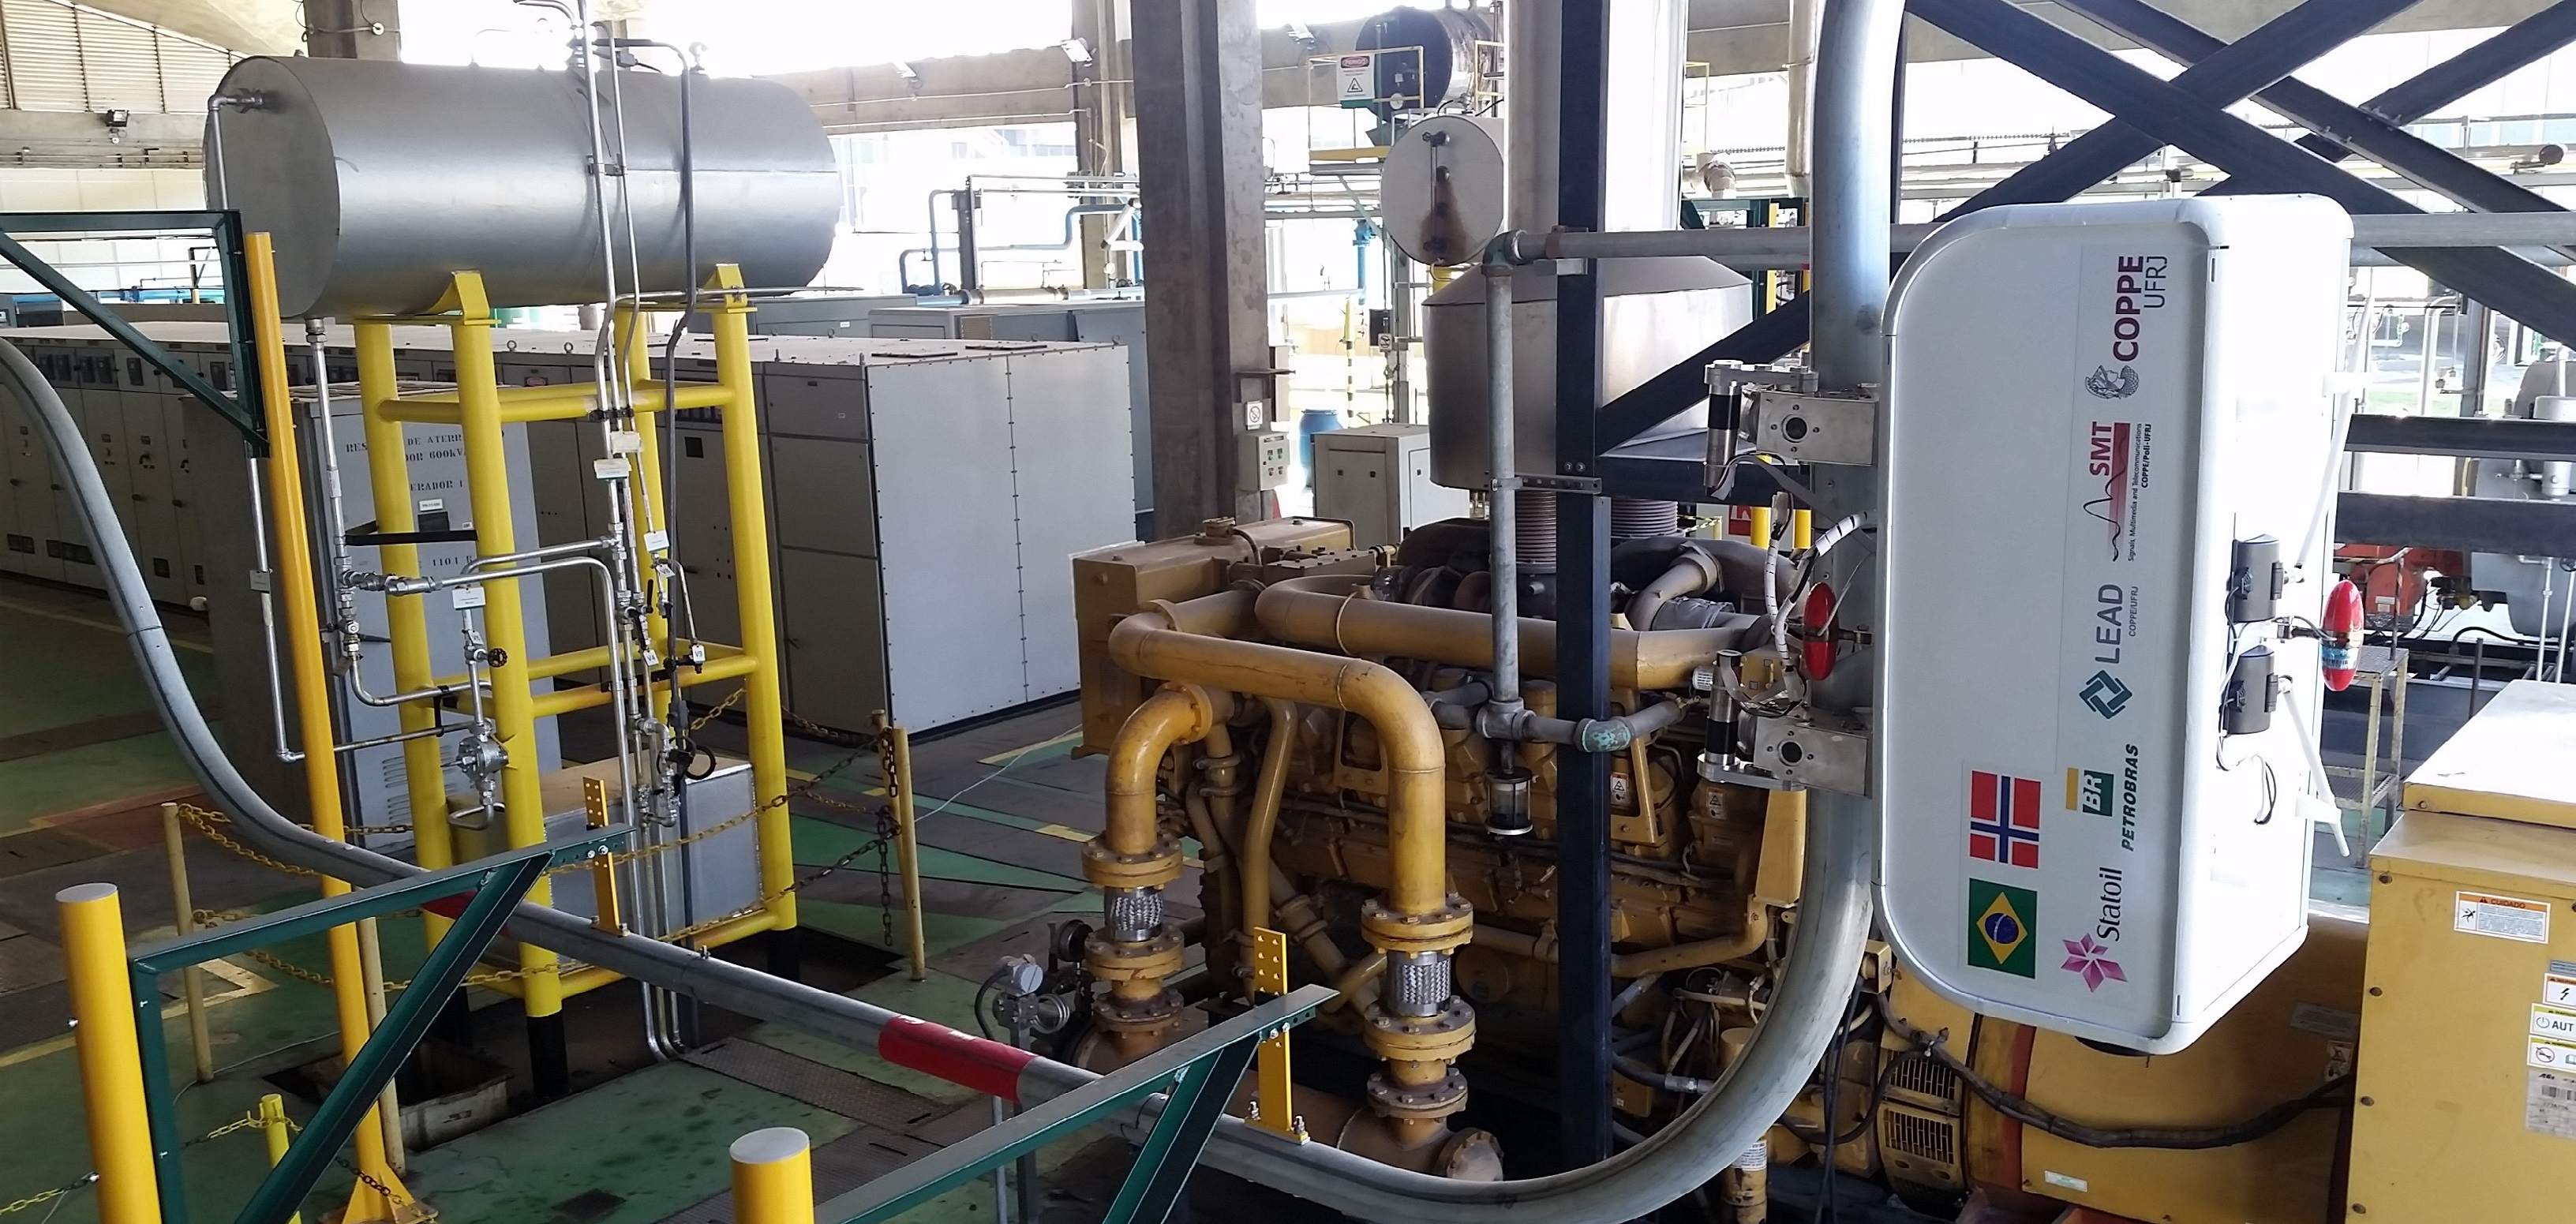
\includegraphics[width=\linewidth]{./img/cenpes_field.jpg}
  \caption{DORIS em operação no CENPES}
  \label{fig:cenpes_doris}
\end{figure}%

\section{Manipulador TETIS}
Considerando as tarefas mencionadas foi proposta a adição de um manipulador leve, de modo a extender o espaço de trabalho do robô. Com esse manipulador, pretende-se solucionar os problemas de
\begin{itemize}
\item mover a câmera acoplada ao efetuador, de modo a posicioná-la melhor ao longo da instalação
\item posicionar um sensor de vibração corretamente sobre a superfície de um equipamento na plataforma
\item interagir com \textit{touchscreens}
\end{itemize}

Foi dado a esse manipulador o nome TETIS. O projeto mecânico permite que ele assuma configurações de juntas diferentes, como mostra a figura \ref{fig:tetis}. 

\newlength{\twosubhtt}
\newsavebox{\twosubboxt}

\begin{figure}[htp]
% preliminary
\sbox\twosubboxt{%
  \resizebox{\dimexpr.9\textwidth-1em}{!}{%
    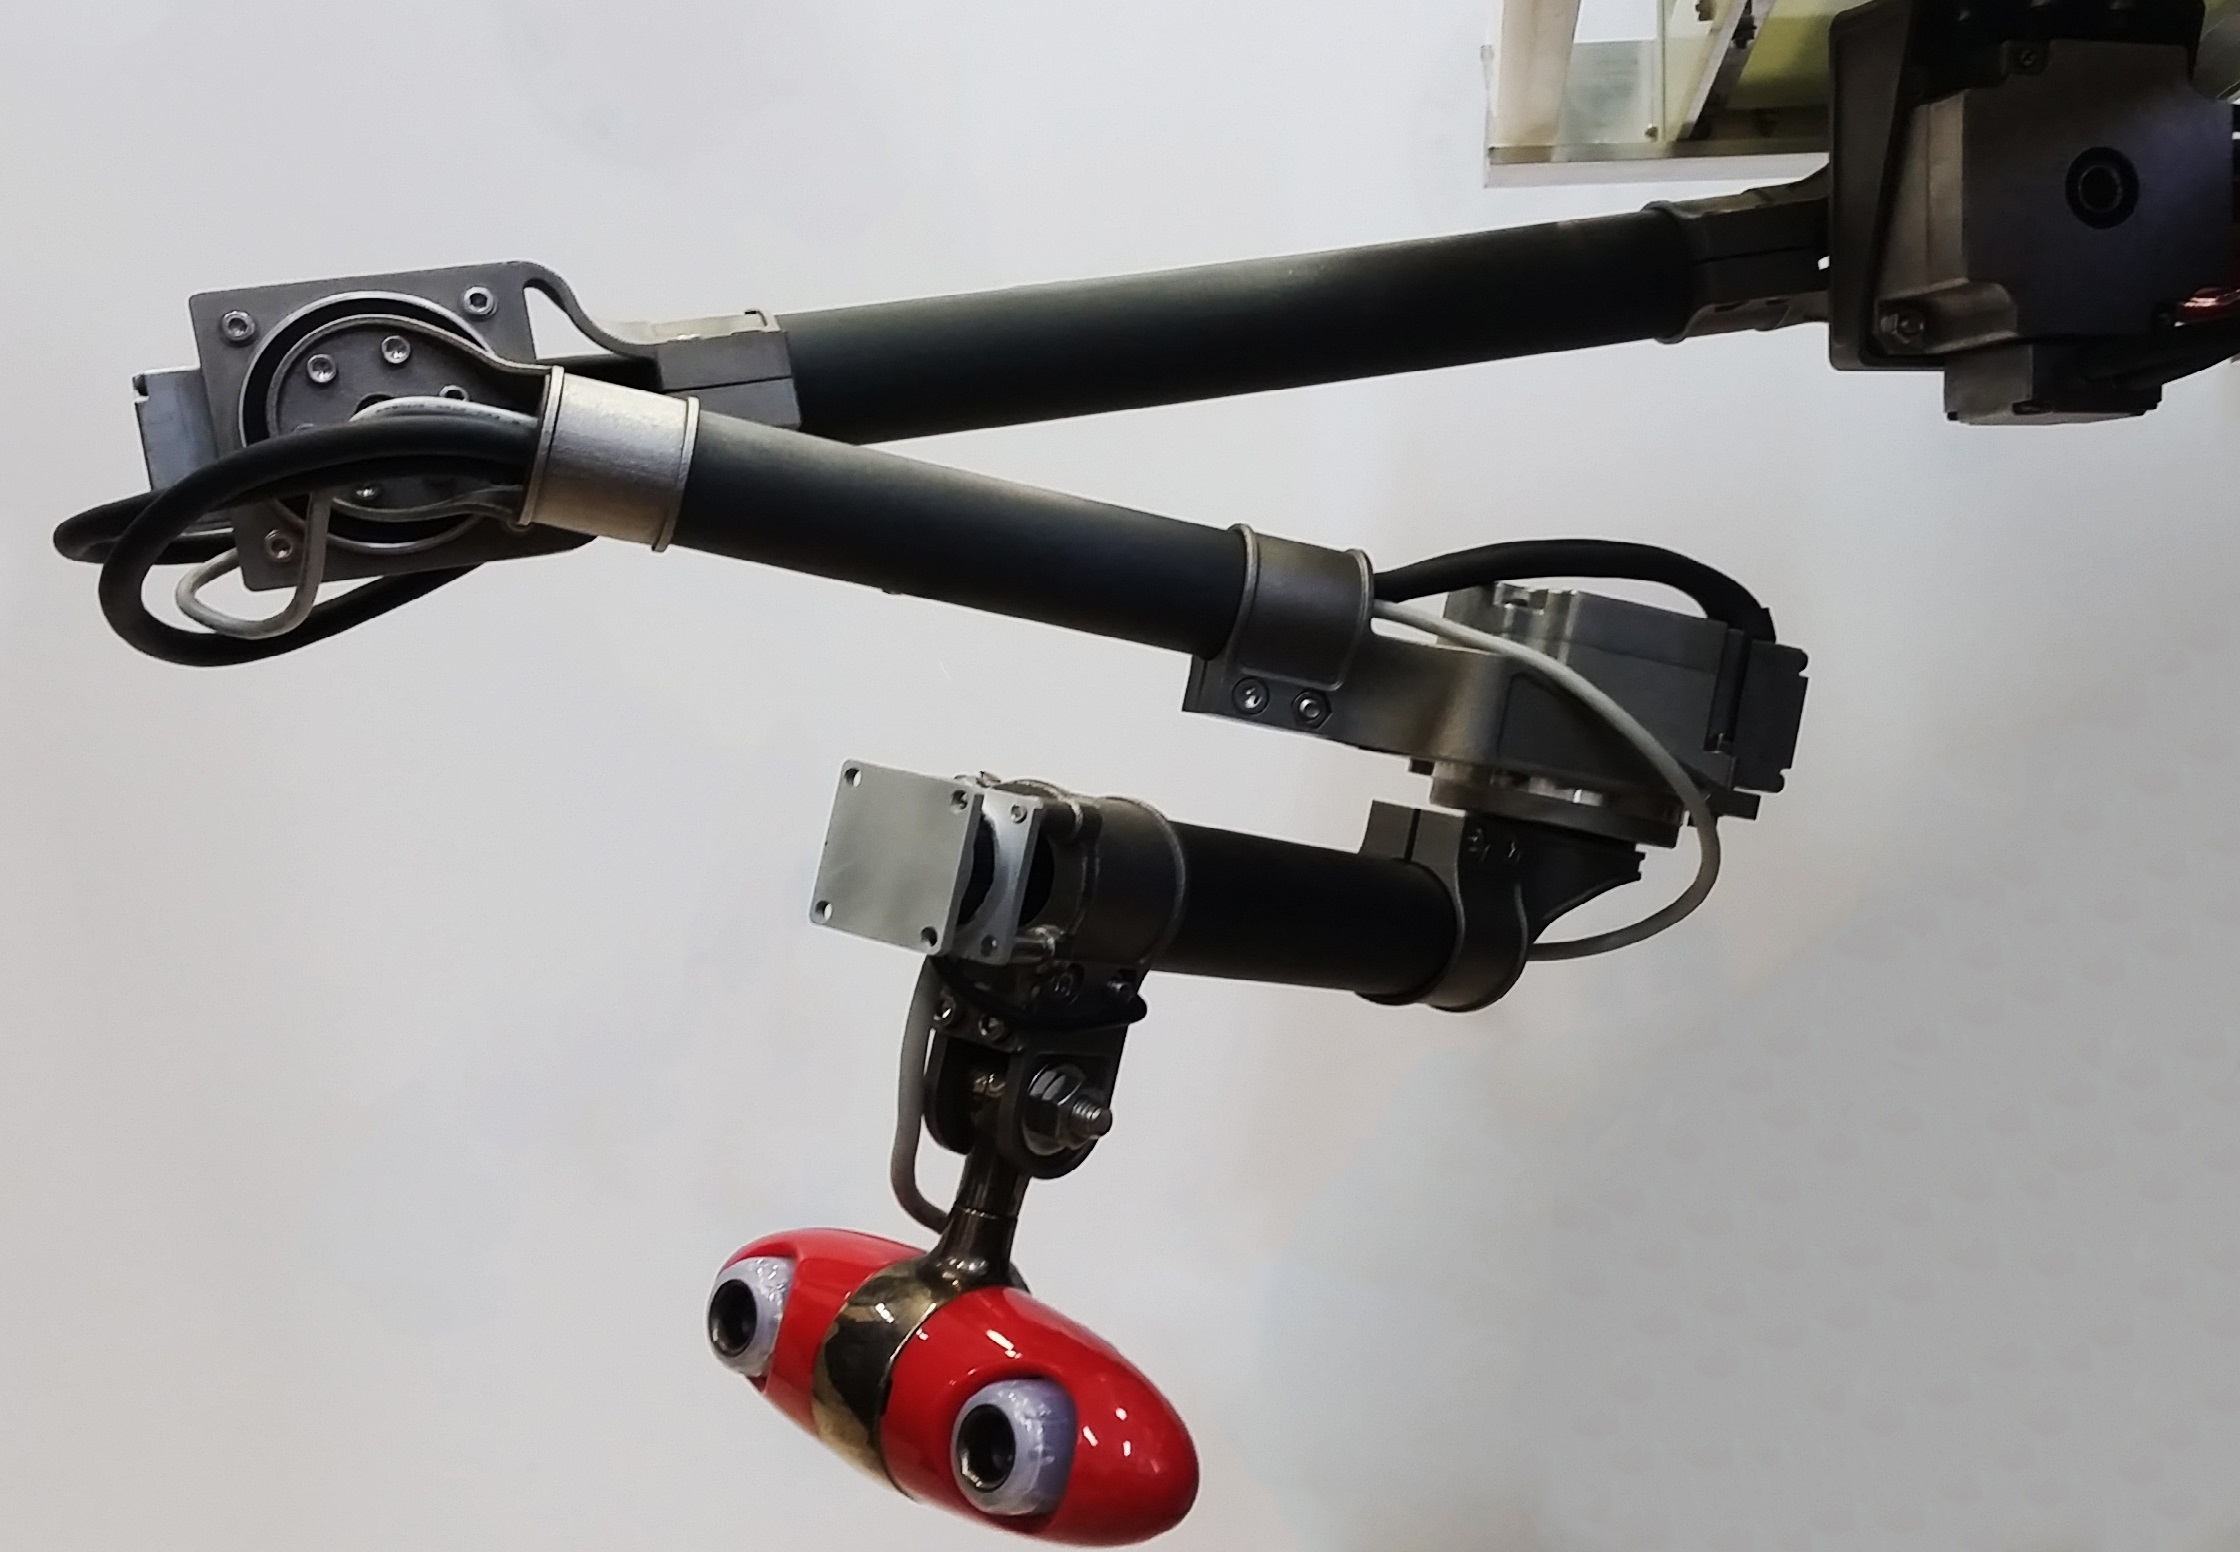
\includegraphics[height=3cm]{./img/manip.jpg}%
    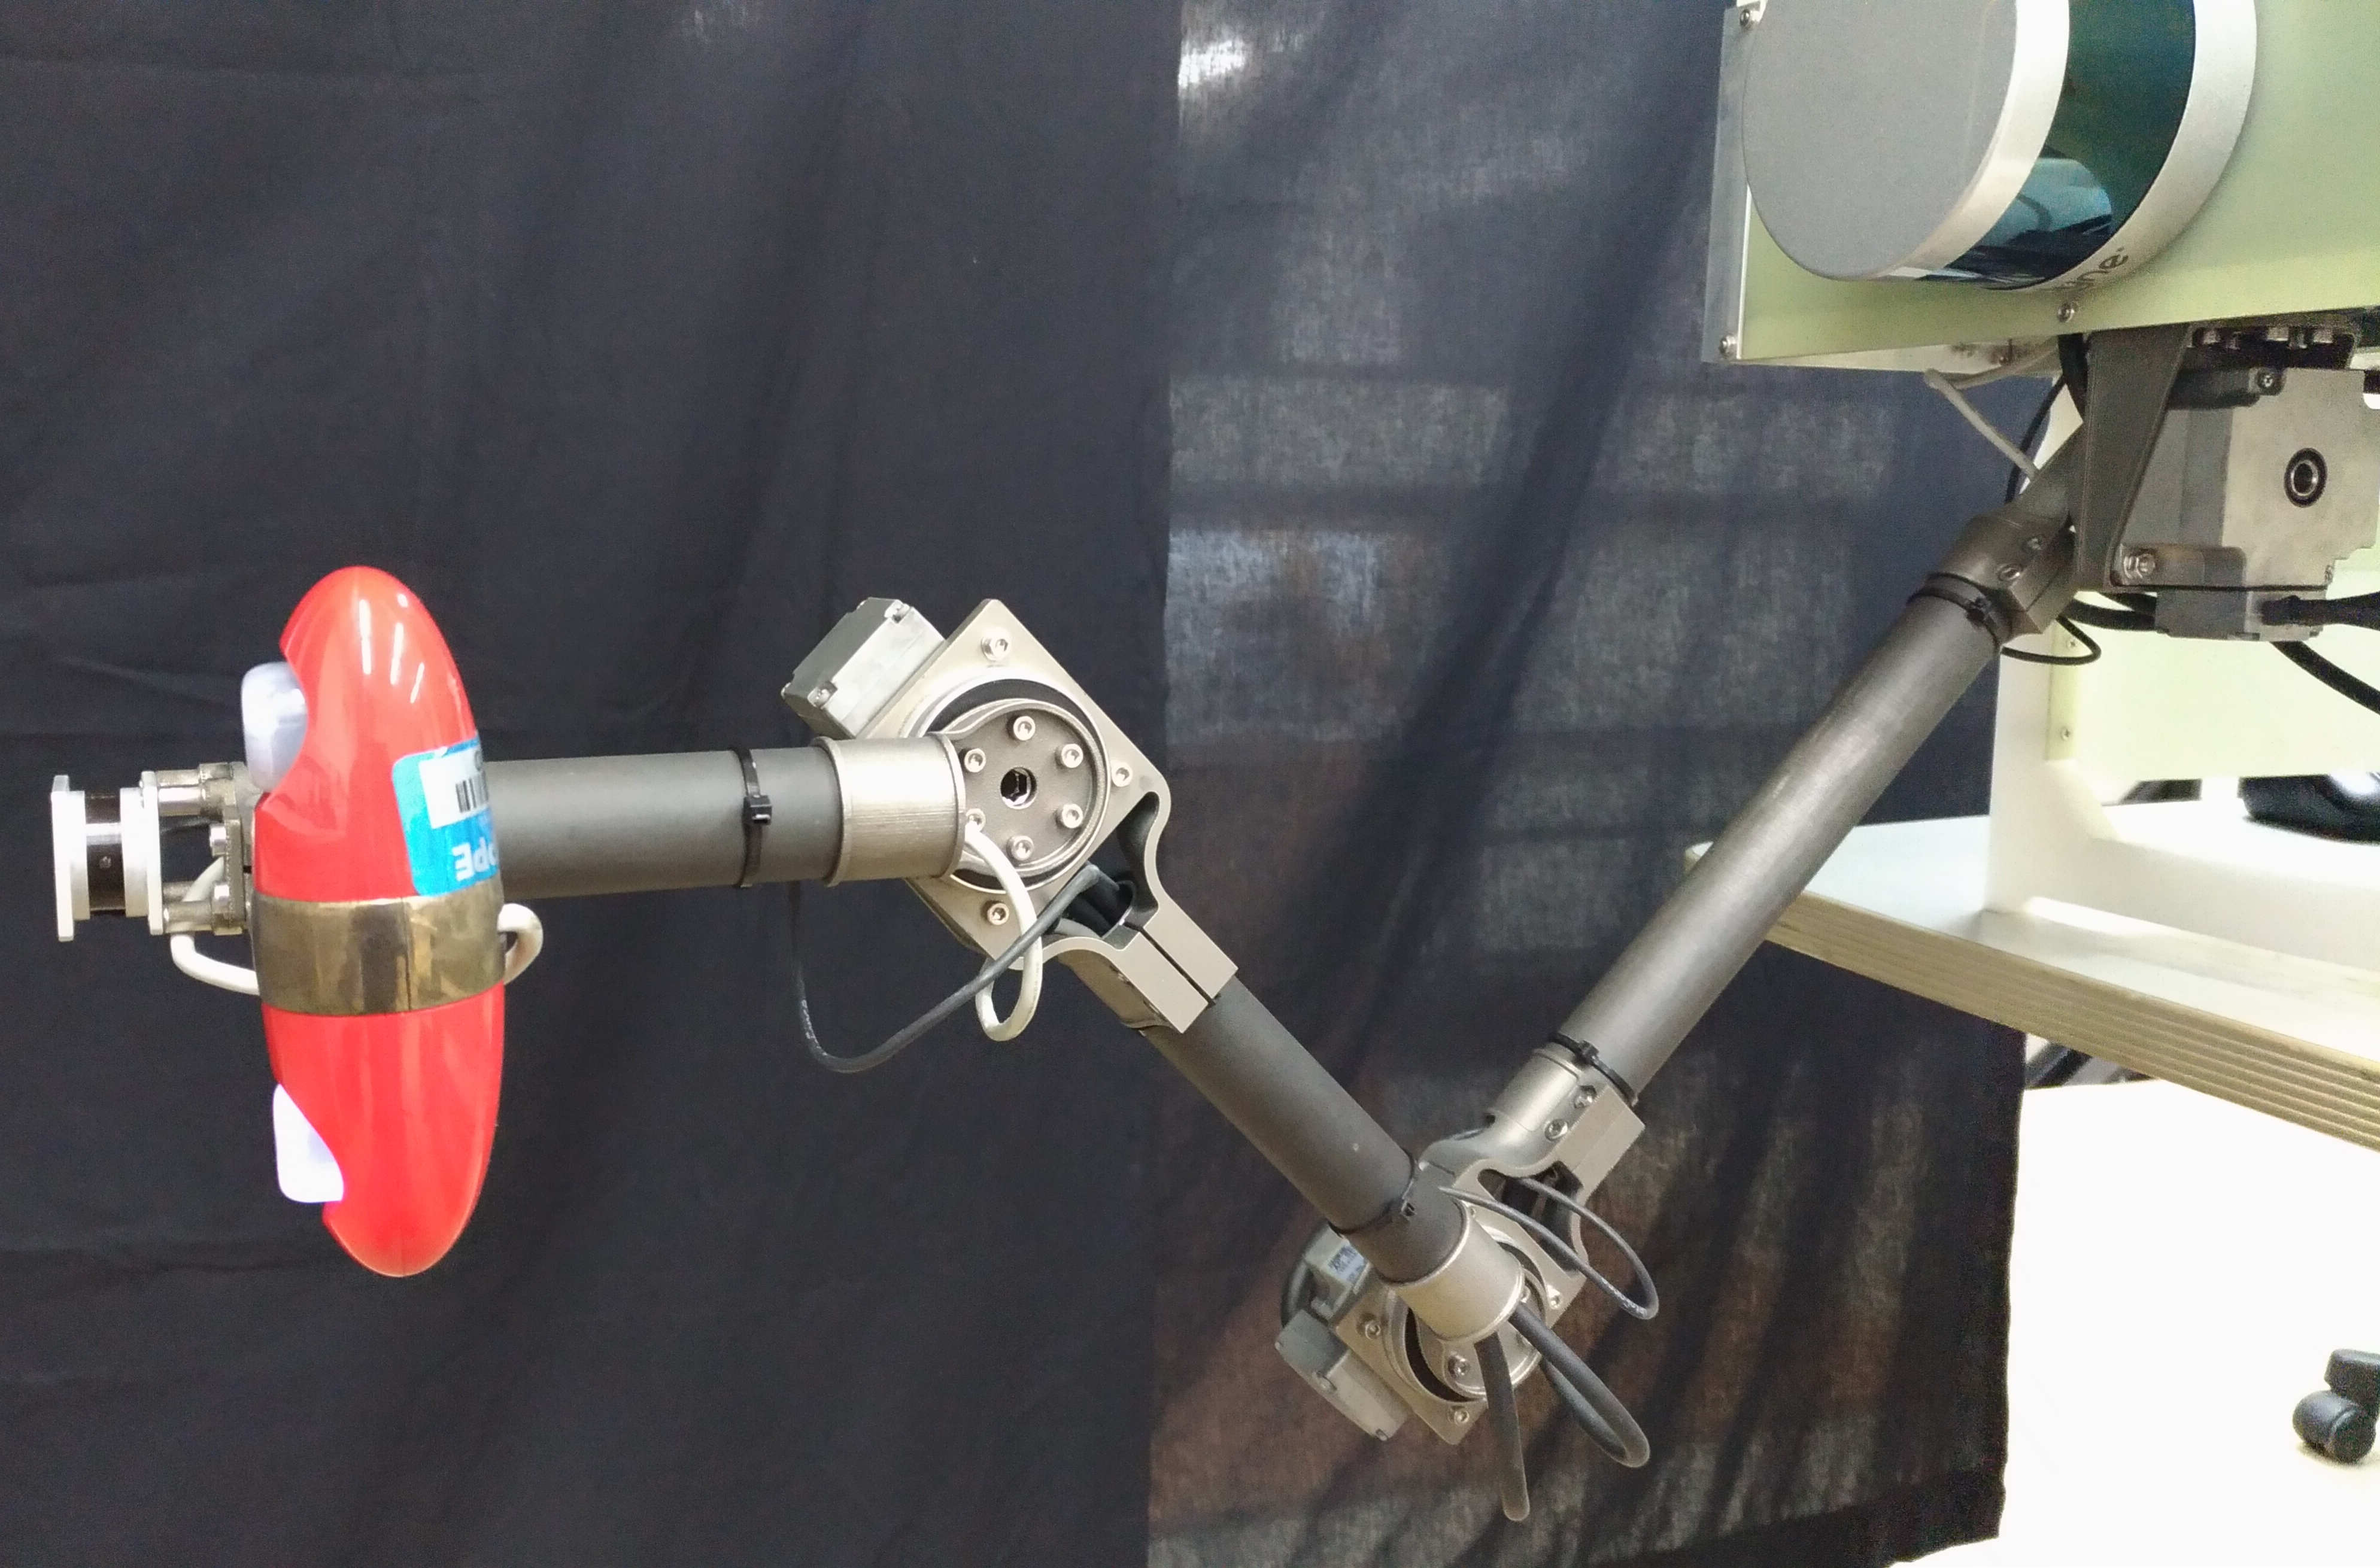
\includegraphics[height=3cm]{./img/manip2.jpg}%
  }%
}
\setlength{\twosubhtt}{\ht\twosubboxt}
% typeset
\centering
\subcaptionbox{Configuração 1\label{fig:tetis1}}{%
  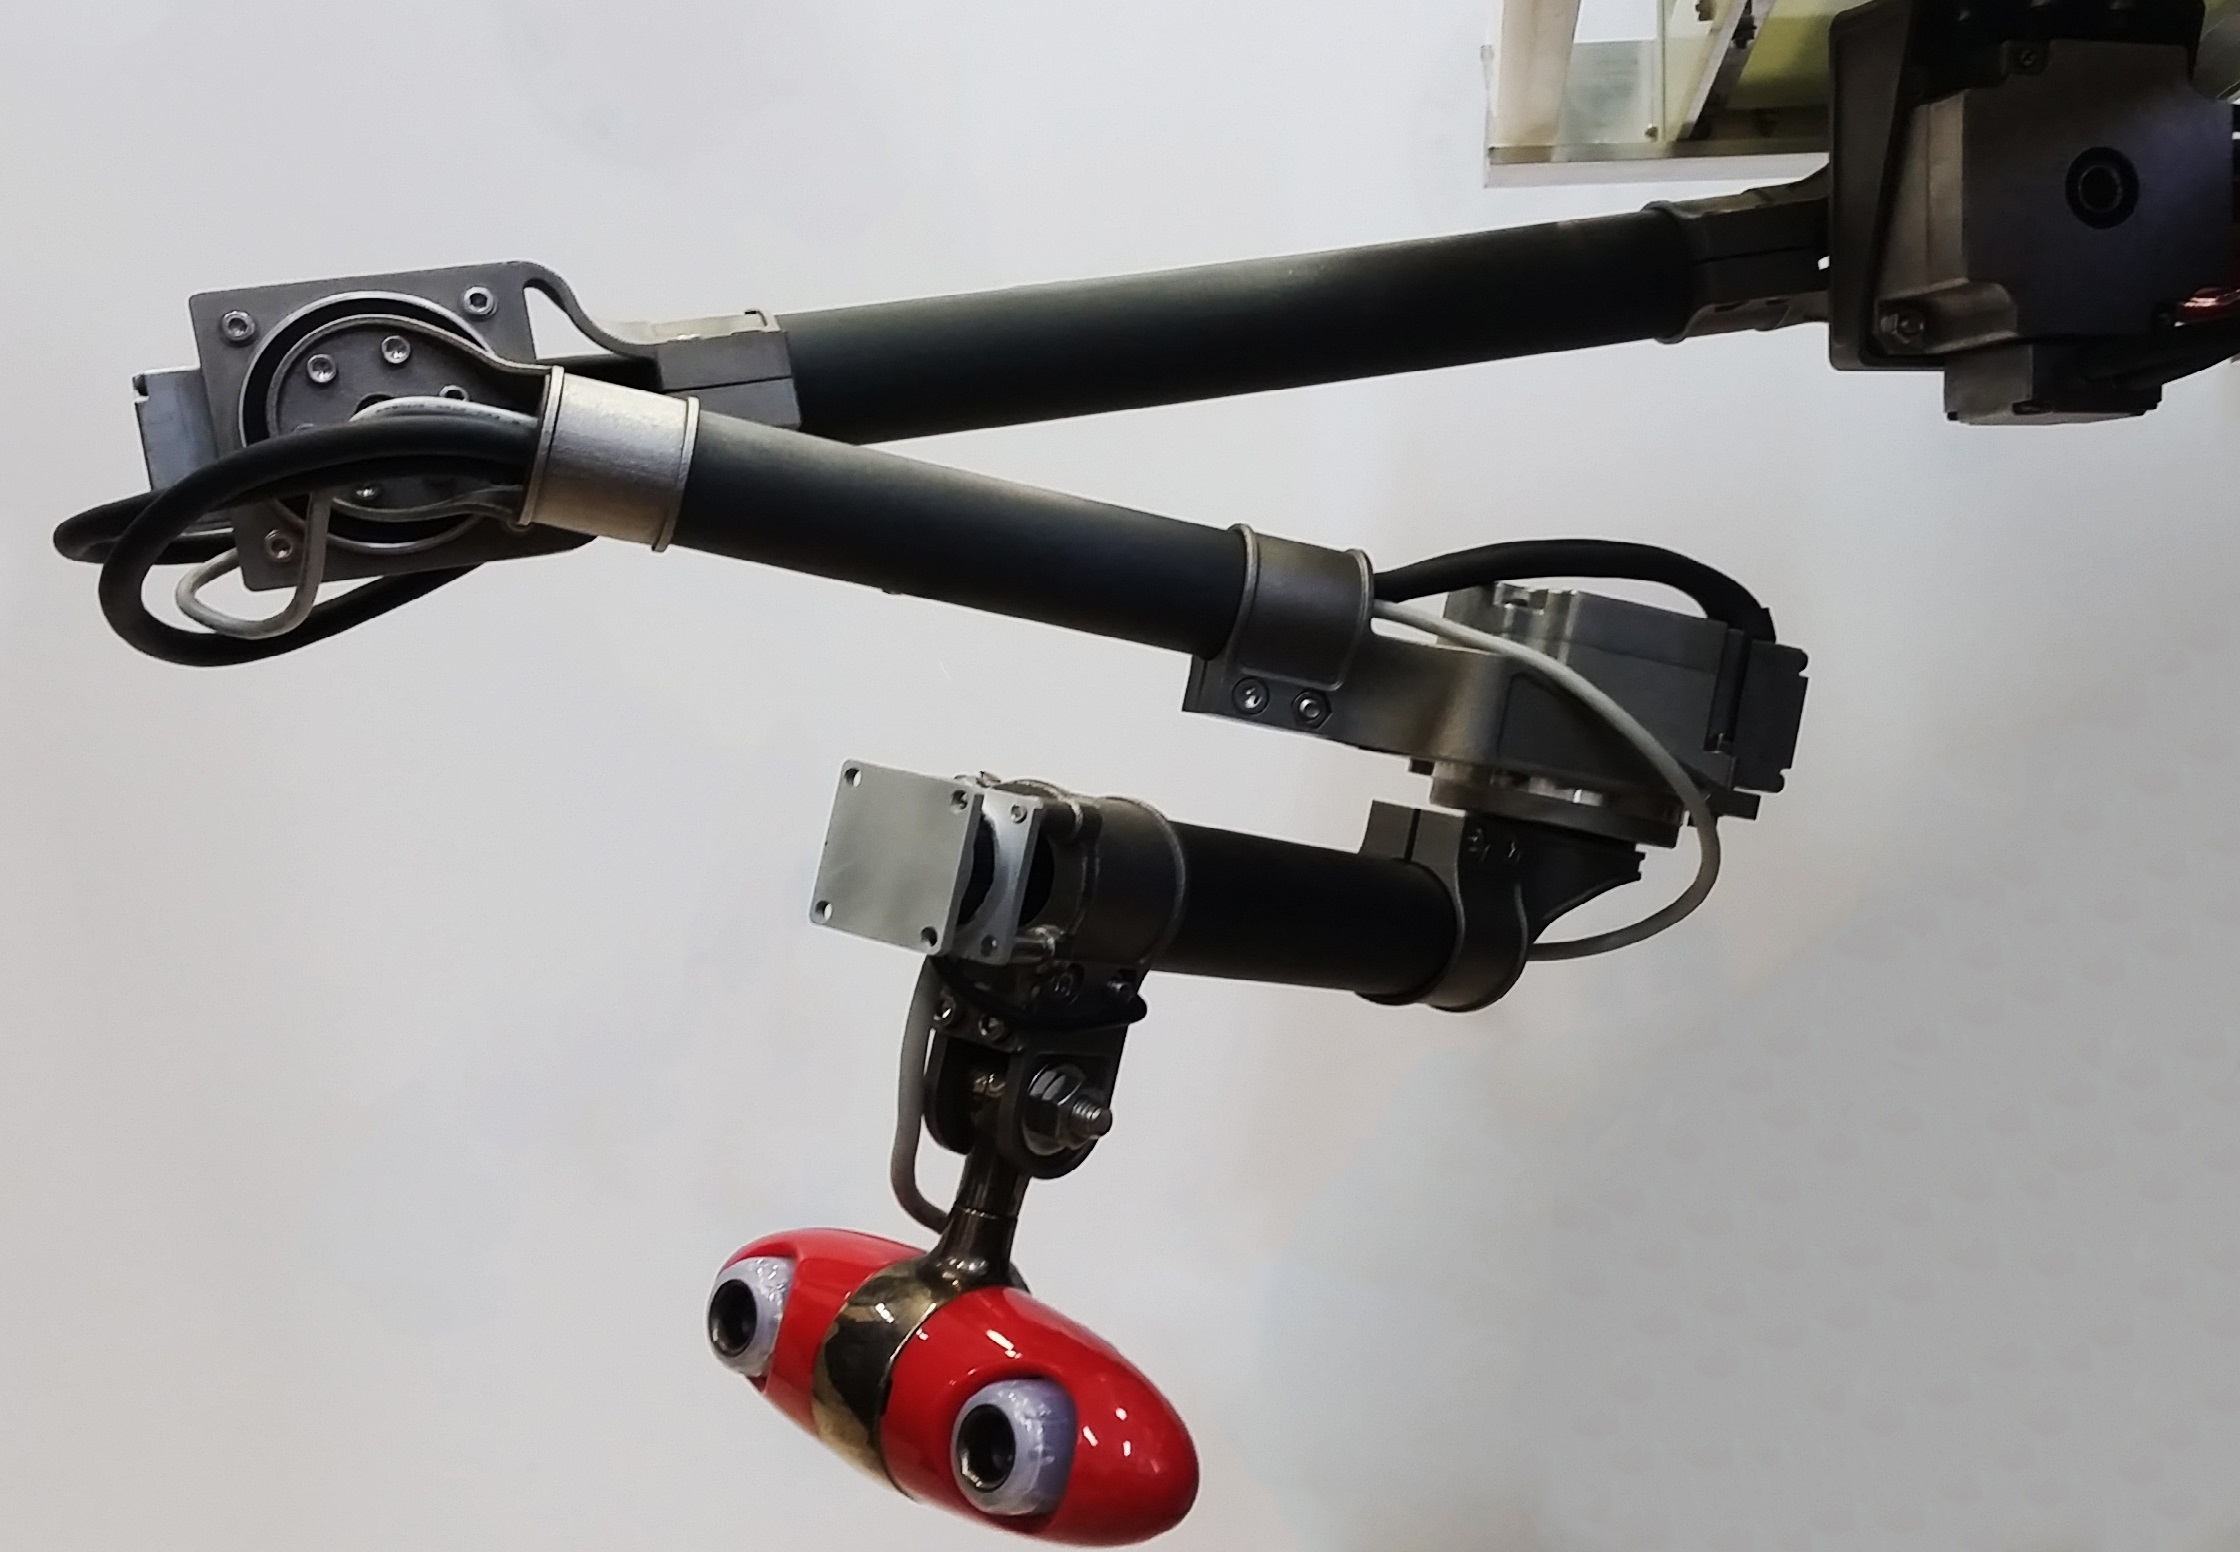
\includegraphics[height=\twosubhtt]{./img/manip.jpg}%
}\quad
\subcaptionbox{Configuração 2\label{fig:tetis2}}{%
  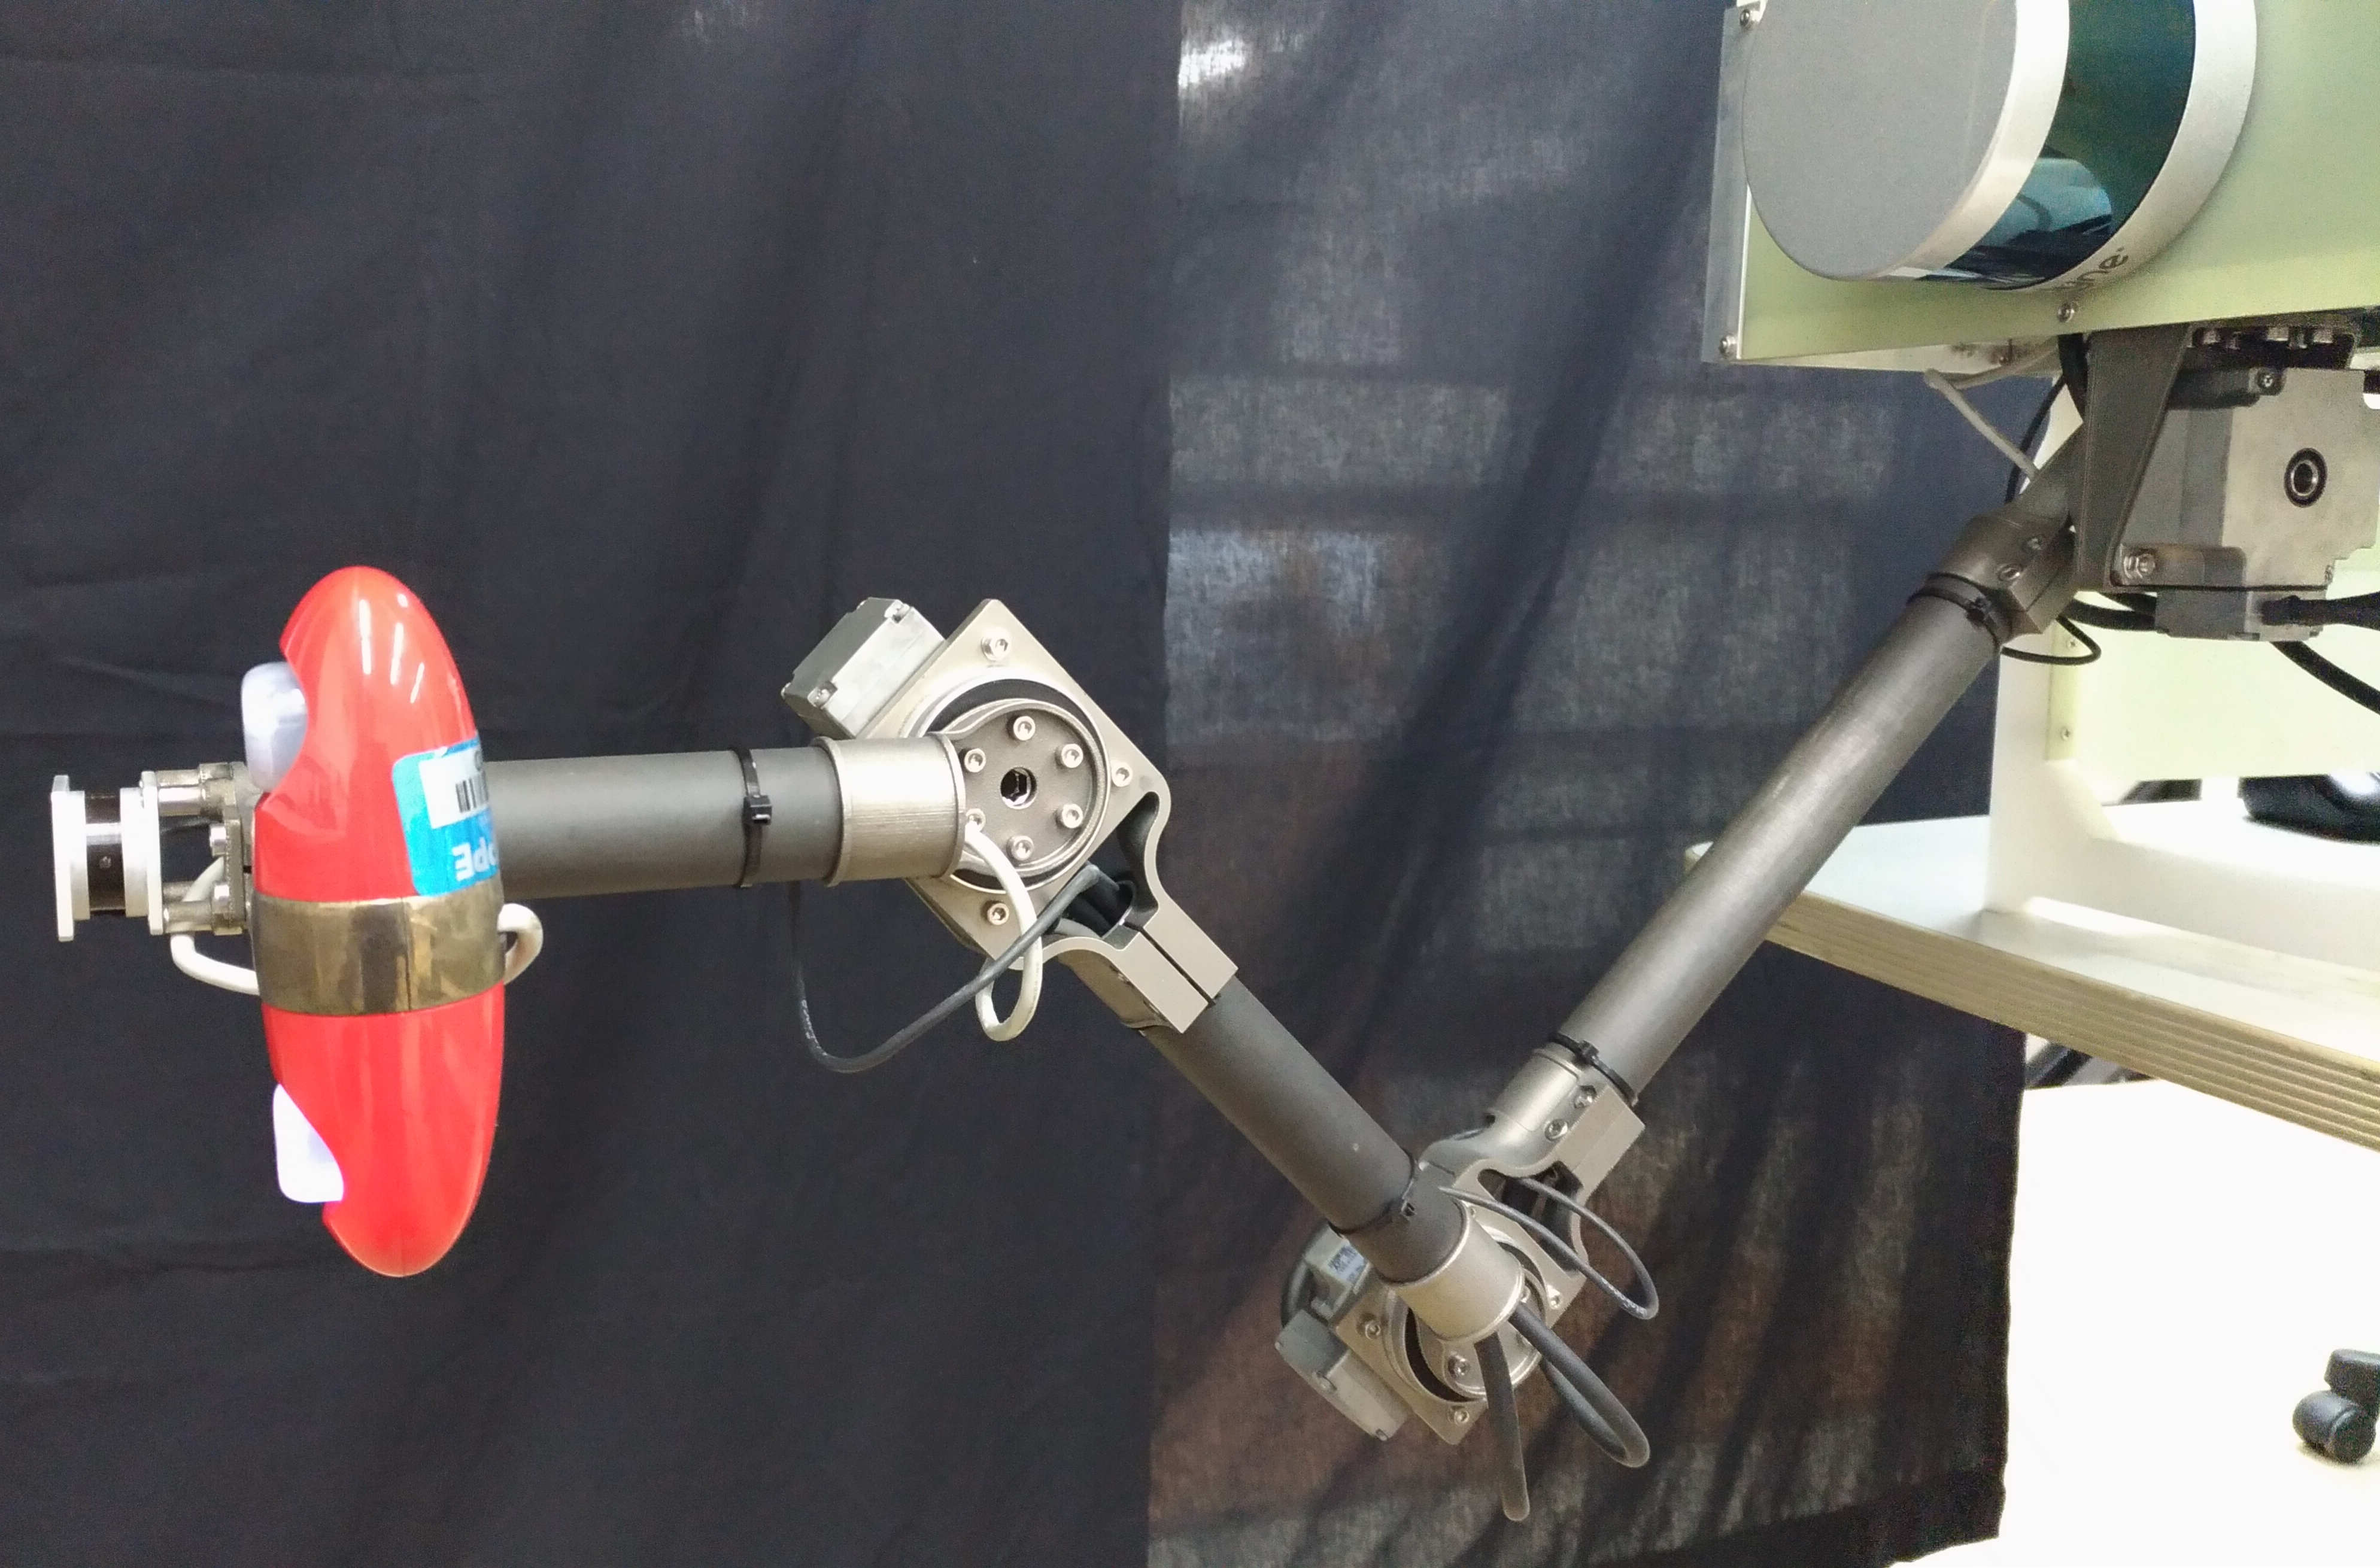
\includegraphics[height=\twosubhtt]{./img/manip2.jpg}%
}
\caption{Manipulador TETIS}
\label{fig:tetis}
\end{figure}

\section{Robot Operating System}
Com sua primeira versão em 2007, o \textit{framework} ROS (Robot Operating System) tem ganhado grande aceitação da comunidade na construção de aplicações para robôs. Consiste em um conjunto de bibliotecas e ferramentas que auxiliam desenvolvimento de software para robótica. Essa não é uma tarefa simples, pois o cada vez mais o escopo dos projetos aumenta, englobando algoritmos de controle, visão computacional, percepção e tomada de decisão.
 %em projetos de robótica.
Dentre as principais filosofias adotadas, destaca-se a modularidade. 
Muitos projetos tem a tendência de englobar código específico para o robô em questão, de modo que torna-se difícil reaproveitar algorítimos úteis. O ROS encoraja a comunidade de contribuidores a desenvolver pacotes que possam ser reutilizados em outros projetos.  

Processos que utilizam ROS são chamados de nós e comunicam entre si através de uma topologia ponto-a-ponto, podendo ser executados na mesma máquina ou em diferentes computadores em uma LAN. Dessa forma, os diferentes componentes necessários para o software de um robô podem ser encapsulados em nós, o que garante uma maior possibilidade de reaproveitamento, facilidade de alteração e versatilidade de execução.


\section{Objetivos}

Com o projeto mecânico do manipulador finalizado, segue a etapa de modelagem e implementação de estratégias de controle. 
Nesse contexto, insere-se este trabalho. Utilizando a configuração do manipulador mostrada na figura \ref{fig:tetis2}, alternativa àquela abordada em \citep{xaud2016doris},  busca-se:
\begin{itemize}
\item Elaborar o modelo cinemático e implementar estratégias de controle. %de posição, rastreamento de trajetória.

\item Utilizar a câmera para controle por servo visão onde o alvo é um marcador em algum ponto de interesse, como por exemplo uma máquina a ser inspecionada. 

\item Com o sensor de força montado no efetuador do manipulador, realizar controle de força sobre uma superfície.

\item A partir do RobotGUI, que já interage com os outros dispositivos do DORIS, desenvolver um software para controle de manipuladores robóticos. O uso do ROS proporciona uma maior versatilidade e facilidade para incorporação de novas funcionalidades, em comparação com abordagens tradicionais.

\item Utilizando \textit{Julia Language} permitir que o algoritmo de controle seja modificado em tempo de execução.
\end{itemize}


\section{Organização do trabalho}

%TODO
No primeiro capítulo o trabalho foi contextualizado, descrevendo os objetivos do projeto DORIS e do manipulador TETIS. No segundo capítulo são mostrados conceitos de robótica necessários para a modelagem e controle de manipuladores robóticos. No capítulo 3 esses conceitos são aplicados ao manipulador TETIS.
No capítulo \ref{chap:descricao_hard} é descrito o hardware do robô DORIS.  No capítulo 5 são abordados detalhes das ferramentas e da arquitetura utilizada para a implementação do software. No capítulo 6, são mostrados e discutidos os resultados de simulação e de testes experimentas para os diferentes modos de controle implementados.  Por último, no capítulo 7 são apresentadas as conclusões sobre o trabalho e pontos para serem abordados em trabalhos futuros.


  %!TEX root = <main.tex>
%\chapter{Revisão Bibliográfica}
\chapter{Modelagem e Controle Cinemático}
Neste capitulo serão abordados os conceitos necessários para modelagem e controle de manipuladores robóticos, focando no que foi utilizado neste projeto, para implementação no manipulador 4-DOF chamado de TETIS. Os tópicos tratados aqui podem ser encontrados em \citep{siciliano, petercorke}.

\section{Posição e Orientação de um Corpo Rígido}

Um corpo rígido é descrito no espaço por sua posição e orientação (pose) em relação a um sistema de coordenadas de referência. Escolhe-se um ponto do corpo e afixa-se um sistema de coordenadas. Denota-se como $\bar{E}$ um sistema de coordenadas ortonormal com $\vec{x}$, $\vec{y}$ e $\vec{z}$ como vetores unitários.

Sejam o sistema de coordenadas inercial $\bar{E}_a = [\vec{x}_a \; \vec{y}_a \; \vec{z}_a ]$ e o sistema de coordenadas do corpo $\bar{E}_b = [\vec{x}_b \; \vec{y}_b \; \vec{z}_b ]$, como mostra a Figura \ref{fig:pose_frames}.

\begin{figure}[!h]
  \centering
  \includegraphics[width=0.4\linewidth]{./img/pose_frames}
  \caption{Sistemas de coordenadas de referência $\bar{E}_a$ e do corpo $\bar{E}_b$.}
  \label{fig:pose_frames}
\end{figure}

A \textbf{posição} da origem $O_b$ do sistema de coordenadas do corpo rígido em relação ao sistema de coordenadas inercial é dada por 
\begin{equation}
p_b = p_{b_x} \vec{x}_a + p_{b_y} \vec{y}_a + p_{b_z} \vec{z}_a, 
\end{equation}
onde $p_{b_x}$, $p_{b_y}$ e $p_{b_z}$ denotam as componentes do vetor $p_b \in \mathbb{R}^3$ representadas no sistema de coordenadas $\bar{E}_a$. Pode ser escrita de forma compacta como um vetor $(3 \times 1)$
\begin{equation}
p_{b} = \m{p_{b_x} \\ p_{b_y} \\ p_{b_z}}
\end{equation}

As coordenadas de $\vec{x}_b$, $\vec{y}_b$ e $\vec{z}_b$ representadas no sistema de coordenadas $\bar{E}_a$ são dadas por $x_{ab}$, $y_{ab}$ e $z_{ab}$ em
\begin{align}
x_{ab} &= \bar{E}_a^* \vec{x}_b  \label{eq:xab} \\
y_{ab} &= \bar{E}_a^* \vec{y}_b \label{eq:yab}\\ 
z_{ab} &= \bar{E}_a^* \vec{z}_b \label{eq:zab}
\end{align}
onde $\bar{E}^* = [\vec{e}_1 \cdot  \;\; \vec{e}_2  \dot \;\; \vec{e}_3 \dot] $ denota o operador adjunto de $\bar{E}$.


A partir das equações \eqref{eq:xab}, \eqref{eq:yab} e \eqref{eq:zab}, podemos escrever:
\begin{align}
\vec{x}_b &= \bar{E}_a x_{ab} \\
\vec{y}_b &= \bar{E}_a y_{ab} \\
\vec{z}_b &= \bar{E}_a z_{ab} ,
\end{align}
portanto,
\begin{equation}
\bar{E}_b = [\bar{E}_a x_{ab} \;\; \bar{E}_a y_{ab} \;\; \bar{E}_a z_{ab}] = \bar{E}_a [x_{ab} \;\;  y_{ab} \;\; z_{ab}] = \bar{E}_a R_{ab}
\end{equation}

A matriz $R_{ab}$ é chamada de matriz de rotação e define a \textbf{orientação} do corpo rígido.
\begin{equation}
R_{ab} = \m{ x_{ab} & y_{ab} & z_{ab} }
\end{equation}
onde $x_{ab} \in \mathbb{R}^3$,  $y_{ab} \in \mathbb{R}^3$ e $z_{ab} \in \mathbb{R}^3$ são as componentes do sistema de coordenadas $\bar{E}_b$ no sistema de coordenadas $\bar{E}_a$, ou seja:
\begin{equation}
R_{ab} =  \m{ \vec{x}_a \cdot \\ \vec{y}_a \cdot  \\ \vec{z}_a \cdot  } \m{ \vec{x}_b & \vec{y}_b & \vec{z}_b } = 
\m{
    (\vec{x}_a \cdot \vec{x}_b) & (\vec{x}_a \cdot \vec{y}_b)& (\vec{x}_a \cdot \vec{z}_b) \\
    (\vec{y}_a \cdot \vec{x}_b)& (\vec{y}_a \cdot \vec{y}_b)& (\vec{y}_a \cdot \vec{z}_b) \\
    (\vec{z}_a \cdot \vec{x}_b) &(\vec{z}_a \cdot \vec{y}_b)& (\vec{z}_a \cdot \vec{z}_b)
}
\end{equation}


\subsection{Representação de um vetor}
%Uma matriz de rotação pode ser interpretada como 
Um vetor $\vec{p}$ pode ser representado como $(p)_a = [p_{x} \;\; p_{y} \;\; p_{z}]$ no sistema de coordenadas $\bar{E}_a$ e como $(p)_b = [p'_{x} \;\; p'_{y} \;\; p'_{z}]$ no sistema de coordenadas $\bar{E}_b$. 
A matriz de rotação $R_{ab}$ representa a transformação de coordenadas de $\vec{p}$ em $\bar{E}_b$ para suas coordenadas em $\bar{E}_a$, através de 
\begin{equation}
(p)_a = R_{ab}(p)_b.
\end{equation}


\subsection{Transformações Homogêneas}
A posição de um corpo rígido é expressa em função da posição de um ponto no corpo rígido com respeito ao sistema de coordenadas de referência (translação),
 enquanto que sua orientação é expressa em termos das componentes dos vetores unitários do sistema de coordenadas do corpo em relação ao sistema de coordenadas de referência (rotação).


\begin{figure}[!h]
  \centering
  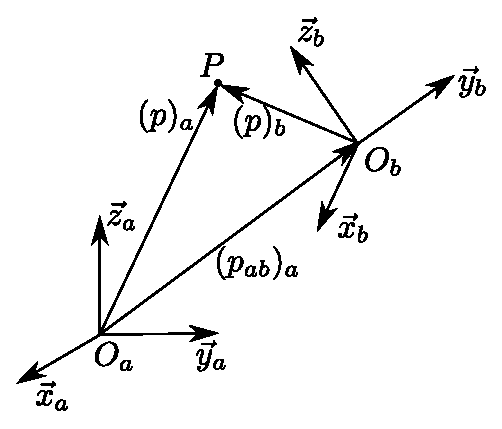
\includegraphics[width=0.4\linewidth]{./img/homogeneous_transform}
  \caption{Representação de um ponto $P$ em diferentes sistemas de coordenadas.}
  \label{fig:homogeneous_transform}
\end{figure}


Seja $(p)_a$ o vetor de coordenadas de um ponto P no espaço, em relação a um sistema de coordenadas de referência $\bar{E}_a = [\vec{x}_a \; \vec{y}_a \; \vec{z}_a ]$. 
Considerando um sistema de coordenadas  $\bar{E}_b = [\vec{x}_b \; \vec{y}_b \; \vec{z}_b]$, seja $(p_{ab})_a$ o vetor de coordenadas descrevendo a origem do sistema de coordenadas $\bar{E}_b$ com relação sistema de coordenadas  $\bar{E}_a$. A matriz de rotação $R_{ab}$ descreve a orientação do sistema de coordenadas $\bar{E}_b$ em relação a $\bar{E}_a$. Seja, também, $(p)_b$ o vetor de coordenadas do ponto $P$ em relação ao sistema de coordenadas $\bar{E}_b$.  A posição do ponto $P$ pode ser representada no sistema de coordenadas de referência como
\begin{equation} \label{eq:transrot}
(p)_a = (p_{ab})_a + R_{ab} (p)_b.
\end{equation}
A Equação \eqref{eq:transrot} representa a transformação de coordenadas (translação e rotação) de um vetor, de um sistema de coordenadas para outro.

De forma a obter uma representação compacta da relação entre as coordenadas de um mesmo ponto em dois sistemas de coordenadas diferentes, introduz-se a representação homogênea de um vetor $p$ como $\tilde{p} \in \mathbb{R}^4$, formado adicionando um quarto componente unitário, ou seja
\begin{equation}
\tilde{p} = \m{p \\ 1}.
\end{equation}  
Adotando essa representação a transformação de coordenadas pode ser escrita através da matriz $(4 \times 4) $
\begin{equation}
T_{ab} = \m{
    R_{ab} & (p_{ab})_a \\
    0_{1 \times 3} & 1
}
\end{equation}

Portanto a transformação de coordenadas de um vetor de $\bar{E}_b$ para $\bar{E}_a$ pode ser expressa de forma compacta por uma única matriz, como
\begin{equation}
(\tilde{p})_a = T_{ab} (\tilde{p})_b
\end{equation}
enquanto que a transformação de $\bar{E}_a$ para $\bar{E}_b$ é descrita pela matriz $T_{ba}$ que satisfaz a equação
\begin{equation}
(\tilde{p})_b = T_{ba} (\tilde{p})_b = (T_{ab})^{-1} (\tilde{p})_a .
\end{equation}
A matriz $T_{ba}$ pode ser expressa como
\begin{equation}
T_{ba} = \m{
    R_{ba} & -R_{ba}(p_{ab})_a \\
    0_{1 \times 3} & 1
}.
\end{equation}

\section{Cinemática Direta}
Um manipulador robótico é composto de uma série de corpos rígidos denominados \textit{elos} conectados através de \textit{juntas}. 
Juntas podem ser:
\begin{itemize} 
\item Revolução
\item Prismática
\end{itemize}

Essa estrutura é chamada de cadeia cinemática.
Um extremo da cadeia é fixado a base e o outro ao efetuador.
Nesse texto serão abordadas apenas cadeias cinemáticas abertas, ou seja, aquelas em que existe apenas uma sequência de elos conectando os dois extremos da cadeia.
Cada junta acrescenta um grau de liberdade (DOF), ao qual está associado a uma variável de junta. No caso de uma junta de revolução um ângulo e no caso de uma junta prismática um deslocamento.
O objetivo da cinemática direta é calcular a posição e orientação do efetuador em função das variáveis das juntas.

%É possível expressar a 

Uma cadeia cinemática aberta é constituída por $n+1$ elos numerados de $0$ a $n$, onde o Elo 0 é fixado a base por convenção. O método utilizado consiste em definir um sistema de coordenadas associado a cada elo e calcular a transformação homogênea entre elos consecutivos. Em seguida a transformação do n-ésimo sistema de coordenadas pode ser obtida de forma recursiva como
\begin{equation}\label{eq:cinedireta}
{T}_{0n}({q}) = {T}_{01}(q_1) {T}_{12}(q_{2}) {\dots} {T}_{n-1,n}(q_n)
\end{equation}
onde ${T}_{i-1,i}(q_i)$ denota a transformação homogênea do sistema de coordenadas solidário ao elo $i-1$ àquele solidário ao elo $i$ e $q \in \mathbb{R}^n$ é o vetor de variáveis de junta, com $n$ sendo o número de juntas.

Logo a transformação homogênea do efetuador final com respeito a base é dada por
\begin{equation} \label{eq:base_efetuador}
{T}_{be}({q}) = {T}_{b0} {T}_{0n}({q}) {T}_{ne} 
\end{equation}

\subsection{Convenção Denavit-Hartenberg} \label{sec:denavit}
Para calcular a cinemática direta para uma manipulador de cadeia cinemática aberta de acordo com a equação \eqref{eq:cinedireta} um método sistemático foi definido para obter a relação entre a posição e orientação de dois elos consecutivos. A convenção Denavit-Hartenberg especifica um conjunto de regras sobre como definir os sistemas de coordenadas de cada elo.

\begin{figure}[!h]
  \centering
  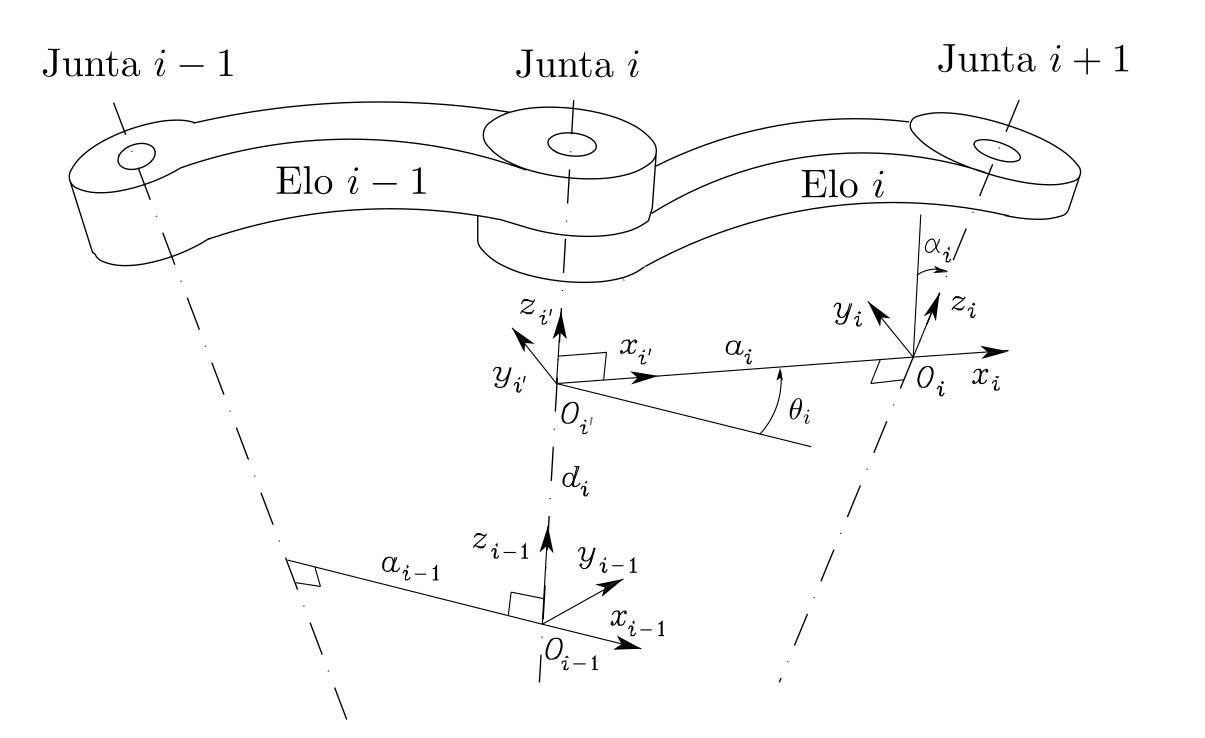
\includegraphics[width=0.8\linewidth]{./img/dh_pt.png}
  \caption{Parâmetros Denavit-Hartenberg.}
  \label{fig:dh_pt}
\end{figure}

Seja o $\vec{h}_i$ eixo de rotação da junta que conecta o elo $i-1$, ao elo $i$, então:

\begin{itemize}
\item Escolher o eixo $\vec{z}_i$ ao longo do eixo $\vec{h}_{i+1}$.
\item Colocar a origem $O_i$ na interseção do eixo $\vec{z}_i$ com a normal comum entre os eixos $\vec{z}_{i-1}$ e $\vec{z}_i$
\item Escolher $\vec{x}_i$ ao longo da normal comum aos eixos $\vec{z}_{i-1}$ e $\vec{z}_i$, com direção da junta $i$ para a junta $i+1$. 
\item O eixo $\vec{y}_i = \vec{z}_i \times \vec{x}_i$ é escolhido de forma a completar o sistema de coordenadas.
\end{itemize}

Essa convenção resulta em uma definição não única do sistema de coordenadas nos seguintes casos:

\begin{itemize}
\item Para o sistema de coordenadas $0$, somente a direção do eixo $\vec{z}_0$ é especificada, portanto a escolha de $O_0$ e $ \vec{x}_0$ é arbitrária.
\item Para o sistema de coordenadas $n$, como não existe junta $n+1$, $\vec{z}_n$ não está definido, mas $\vec{x}_n$ deve ser normal ao eixo $\vec{z}_{n-1}$. Tipicamente escolhe-se $\vec{z}_n$ alinhado com $\vec{z}_{n-1}$.
\item Quando dois eixos consecutivos são paralelos, a normal comum entre eles não é definida de forma única. Tipicamente escolhe-se $O_i$ na junta $i+1$
\item  Quando dois eixos consecutivos se interceptam, direção de $\vec{x}_i$ é normal e o sentido é arbitrário. Escolhe-se $O_i$ na intersecção.
\item Quando a junta $i$ é prismática a direção de $\vec{z}_{i-1}$ é arbitrária.
\end{itemize}

Após determinados os sistemas de coordenadas, é possível determinar a posição e orientação de um referencial em relação ao outro através dos seguintes parâmetros:
\begin{itemize}
\item $a_i$ distância entre $\vec{z}_{i-1}$ e $z_i$ ao longo de $\vec{x}_i$
\item $\alpha_i$ ângulo entre $\vec{z}_{i-1}$ e $\vec{z}_i$ ao redor de $\vec{x}_i$
\item $d_i$ distância entre $\vec{x}_{i-1}$ e $\vec{x}_i$ ao longo de $\vec{z}_{i-1}$
\item $\theta_i$ ângulo entre $\vec{x}_{i-1}$ e $\vec{x}_i$ ao redor de $\vec{z}_{i-1}$
\end{itemize}

A orientação de um sistema de coordenadas $i$ em relação ao anterior é dada por uma rotação de $\theta_i$ em torno de $\vec{z}$ seguida de uma rotação em torno de $\vec{x}$ de $\alpha_i$ considerando o sistema de coordenadas corrente.

\begin{equation}
{R}_{i-1,i} = {R}_z(\theta_i){R}_x(\alpha_i)
\end{equation}

A translação é obtida representando as distâncias no sistema de coordenadas $i-1$:
\begin{gather}
{\vec{p}}_{i-1,i} = d_i {\vec{z}}_{i-1} + a_i {\vec{x}}_i \\
({\vec{p}}_{i-1,i})_{i-1} = d_i ({\vec{z}}_{i-1})_{i-1} + a_i ({\vec{x}}_i)_{i-1} \\
({\vec{p}}_{i-1,i})_{i-1} = d_i ({\vec{z}}_{i-1})_{i-1} + a_i {R}_{i-1,i}({\vec{x}}_i)_{i} 
\end{gather}

As duas informações podem ser representadas de uma forma mais compacta como transformação homogênea:
\begin{equation}
T_{i-1,i} = \m{
    R_{i-1,i}       &  ({\vec{p}}_{i-1,i})_{i-1} \\
    0_{1 \times 3}  &                             1
}
\end{equation}
que em função dos parâmetros fica:
\begin{equation} \label{eq:transform_dh}
T_{i-1,i} = \m {
    c_{\theta_i}  & -s_{\theta_i}c_{\alpha_i}   &   s_{\theta_i}s_{\alpha_i}  & a_i c_{\theta_i} \\ 
    s_{\theta_i}  & c_{\theta_i}c_{\alpha_i}    &  -c_{\theta_i}s_{\alpha_i}  & a_i s_{\theta_i} \\
    0             & s_{\alpha_i}                &   c_{\alpha_i}              & d_i              \\
    0             & 0                           &   0                         & 1
}
\end{equation}
onde utiliza-se a notação $s_i$ para $\sin \theta_i$ e $c_i$ para $\cos \theta_i$. No caso de  $\sin (\theta_i + \theta_j)$ denota-se $s_{ij}$.

\subsection{Espaço das Juntas e Espaço Operacional}
Para que o efetuador final de um manipulador realize alguma tarefa é necessário atribuir uma posição e orientação desejada, que  pode ser função do tempo (trajetória). Surge então o problema de representar posição e orientação. 

Para descrever a posição utiliza-se as coordenadas cartesianas. Para a orientação adota-se uma representação mínima (ângulos de Euler), descrevendo a rotação do efetuador em relação ao sistema de coordenadas da base. Portanto é possível descrever a \textit{pose} do efetuador com relação a base através do vetor
\begin{equation} \label{eq:op_space}
{x}_{be} = \m{ {p}_{be} \\ {\phi}_{be}}
\end{equation}
onde ${p}_{be} \in \mathbb{R}^3$ descreve a posição e ${\phi}_{be} \in \mathbb{R}^3$ é uma representação mínima da orientação.

O \textit{espaço das juntas} denota o espaço em que o vetor $(n \times 1)$ das variáveis das juntas
\begin{equation} \label{eq:joint_space}
{q} = \m{q_1 \\ \vdots \\ q_n}
\end{equation} 
é definido. Se a junta é de revolução utiliza-se $q_i = \theta_i$, se é prismática $q_i = d_i$.

\section{Cinemática Diferencial}
%\subsection{Jacobiano Geométrico}
%Para um manipulador de $n$ graus de liberdade a cinemática direta pode ser escrita como

\subsection{Jacobiano Analítico}
Quando a posição e orientação do efetuador são dadas em função de um número mínimos de parâmetros no espaço operacional é possível computar o Jacobiano pela diferenciação das equações da cinemática direta em função das variáveis das juntas.
Para isso utiliza-se a técnica analítica.

Seja ${p}_{be} \in \mathbb{R}^3$ a posição do sistema de coordenadas do efetuador representada no sistema de coordenadas da base. O vetor $\dot{{p}}_{be}$ é portanto a velocidade de translação, ou linear.
\begin{equation} \label{eq:jacob_pos}
\dot{{p}}_{be} = \frac{\partial {p}_{be} }{\partial {q}} {\dot{q}} = {J}_{ap} ({q}) {\dot{q}} 
\end{equation}
onde ${J}_{ap} \in \mathbb{R}^{3 \times n} $ denota o Jacobiano analítico de posição.

%Para a velocidade angular, pode ser considerada uma representação mínima da orientação em função de três variáveis ${\phi_e}_i$ com $i=1,2,3$. 
A derivada no tempo $\dot{{\phi}}_{be}$ não é igual a velocidade angular, no entanto, conhecida a função ${\phi}_{be}({q})$:

\begin{equation} \label{eq:jacob_or}
\dot{{\phi}}_{be} = \frac{\partial {\phi}_{be}}{\partial {q}} {\dot{q}} = {J}_{a\phi}({q}){\dot{q}}
\end{equation}
onde ${J}_{a\phi}  \in \mathbb{R}^{3 \times n} $ denota o Jacobiano analítico de orientação. Assim, a cinemática diferencial pode ser obtida como:
\begin{equation} \label{eq:jacoba}
\dot{x}_{be} = \m{ \dot{p}_{be} \\ \dot{\phi}_{be} } = \m{ J_{a_p}(q) \\ J_{a_\phi}(q)} {\dot{q}} = {J}_a ({q}) \dot{{q}}
\end{equation}
onde ${J}_{a}  \in \mathbb{R}^{6 \times n} $.
 
\section{Controle Cinemático} \label{sec:controle_cinematico}
O estratégia de controle cinemático pode ser aplicada quando considera-se que a dinâmica do manipulador pode ser desprezada. Essa hipótese se sustenta quando as seguintes premissas são válidas:
\begin{itemize}
\item Elevados fatores de redução nas juntas.
\item Baixas velocidades na realização das tarefas.
\item Existência uma malha de controle de velocidade de alto desempenho em cada junta.
\end{itemize}

\begin{figure}[h!]
\centering
\begin{tikzpicture}[auto, node distance=2cm,>=latex']
    % We start by placing the blocks
    \node [input, name=input] {};
    \node [sum, right of=input] (sum) {};
    \node [block, right of=sum] (K) {$K$};
    \node [block, right of=K] (PWM) {PWM};
    \node [block, right of=PWM] (Robo) {Robô};
    \node [block, right of=Robo] (JA) {${J}_a^{-1}$};
    \node [block, right of=JA] (Integral) {$\int$};
    \node [tmp, below of=K] (tmp1){};
    \node [output, right of=Integral] (output) {};

    % Once the nodes are placed, connecting them is easy. 
    \draw [draw,->] (input) -- node[pos=0.3] {$u$} node[pos=0.8] {$+$} (sum);
    \draw [->] (sum) -- node {$e$} (K);
    \draw [->] (K) -- node {$v$} (PWM);
    \draw [->] (PWM) -- node [name=tau] {$\tau$} (Robo);
    \draw [->] (Robo) -- node [name=dtheta] {$\dot{q}$} (JA);
    \draw [->] (JA) -- node {$\dot{x}_{be}$} (Integral);
    \draw [->] (Integral) -- node [name=x] {$x_e$}(output);
    \draw [->] (dtheta) |- (tmp1)-| node[pos=0.99] {$-$} (sum);
\end{tikzpicture}
\caption{Diagrama de Blocos: Malha de Controle de Velocidade a nível de juntas.}
\label{fig:controlejuntas}
\end{figure}

A maioria dos manipuladores possui uma malha de controle de velocidade em nível de juntas como na Figura \ref{fig:controlejuntas}. Logo, para um controle de alto ganho temos que:
\[ {u} \approx \dot{{q}}\]



Portanto é possível implementar o controle cinemático segundo o diagrama da Figura \ref{fig:controlecinematico}, considerando que o manipulador tem 6 juntas, i.e. $n=6$.

\begin{figure}[h!]
\centering
\begin{tikzpicture}[auto, node distance=2cm,>=latex']
    % We start by placing the blocks
    \node  [input, name=input2] {};
    \node at (0,-1) [input, name=input] {};
    \node [sum, right of=input] (sum) {};
    \node [block, right of=sum] (K) {${K}$};
    \node [sum, right of=K, node distance=2cm] (sum2) {};
    \node [tmp, above of =sum2, node distance=1cm] (tmp1){};
    \node [block, right of=sum2] (JA) {${J}_a^{-1}$};
    \node [block, below of=JA] (k) {${k}(\cdot)$};
    \node [block, right of=JA] (Integral) {$\int$};
    \node [tmp, above of=JA, node distance=1cm] (tmp2){};
    \node [output, right of=Integral] (output) {};

    % Once the nodes are placed, connecting them is easy. 
    \draw [draw,->] (input) -- node[pos=0.3] {${x}_d$}  node[pos=0.8] {$+$} (sum);
    %\draw [draw,->] (input2) -- node {$u$} (sum2);
    \draw [draw,->] (input2) -- node [pos=0.1] {${\dot{x}}_d$} (tmp1)-| node [pos=0.8,anchor=left,left] {$+$} (sum2);
    \draw [->] (sum) -- node {${e}$} (K);
    \draw [->] (K) -- node {}  node[pos=0.8] {$+$} (sum2);
    \draw [->] (sum2) -- node [name=tau]  {} (JA);
    \draw [->] (JA) -- node [name=dtheta] {$\dot{{q}}$} (Integral);
    \draw [->] (Integral) -- node [name=x] {${q}$}(output);
    \draw [->] (x) |- (k);
    \draw [->] (k) -| node[pos=0.99] {$-$} node [near end] {${x}_{be}$} (sum);
    \draw [->] (x) |- (tmp2) -| (JA);
    %\draw [->] (output) |- (tmp1)-| node[pos=0.99] {$-$} (sum);
\end{tikzpicture}
\caption{Diagrama de Blocos: Controle cinemático proporcional com feedforward}
\label{fig:controlecinematico}
\end{figure}


Se ${x_{be}} \in \mathbb{R}^6$ é uma representação da posição e orientação e ${x}_d$ o valor desejado nessa representação, seja o erro no espaço operacional:
\begin{equation}
{e} = {x}_d - {x}_{be}
\end{equation}
Derivando em relação ao tempo
\begin{equation}
{\dot{e}} = {\dot{x}}_d - {\dot{x}_{be}}
\end{equation}
podemos escrever a partir da equação \ref{eq:jacoba}:
\begin{equation}
{\dot{e}} = {\dot{x}}_d - {J}_a({q})\dot{{q}}
\end{equation}
Sendo ${x}_d(t)$ uma trajetória desejada, deseja-se que ${x}_{be}$ atinja ${x}_d(t)$ em $t \to \infty$ .
A entrada de controle para o sistema é um valor de ${u} = \dot{{q}}$, logo, assumindo que ${J}_a({q})$ é quadrada e não singular, a escolha da lei de controle
\begin{equation}
{u} = {J}_a^{-1}({q})\bar{{u}}
\end{equation}
leva ao sistema linear:
\begin{equation}
\dot{{e}} = \dot{{x}}_d - \bar{{u}}
\end{equation}
Se for escolhido $\bar{{u}}$:
\begin{equation}
\bar{{u}} = \dot{{x}}_d + {K_t} ({x}_d - {x}_{be})
\end{equation}
obtem-se a seguinte dinâmica para o erro
\begin{equation}
\dot{{e}} + {K_t} {e} = 0
\end{equation}
onde $K_t = k_t I$. Se $k_t > 0$ o sistema é assintoticamente estável, com $e \rightarrow 0$ quando $t \to \infty$.

\section{Servovisão}
A tarefa proposta na Servovisão é controlar a posição e orientação do efetuador do manipulador, em relação a um alvo, usando características visuais extraídas de uma imagem. A câmera pode ser carregada pelo manipulador (montada no efetuador) ou colocada em um ponto fixo, observando tanto o efetuador como o alvo.

Primeiramente é importante entender os princípios de formação de imagem através de câmeras \citep{petercorke}. 

\subsection{Transformação de Perspectiva} \label{sec:camera_model}
A equação elementar para descrever a formação de imagem com uma lente é a Lei das Lentes
\begin{equation} 
\frac{1}{z_o} + \frac{1}{z_i} = \frac{1}{f}
\end{equation} 
onde $z_o$ é a distância até o objeto, $z_i$ é a distância ao plano da imagem e $f$ é a distância focal da lente.

\begin{figure}[h!]
  \centering
  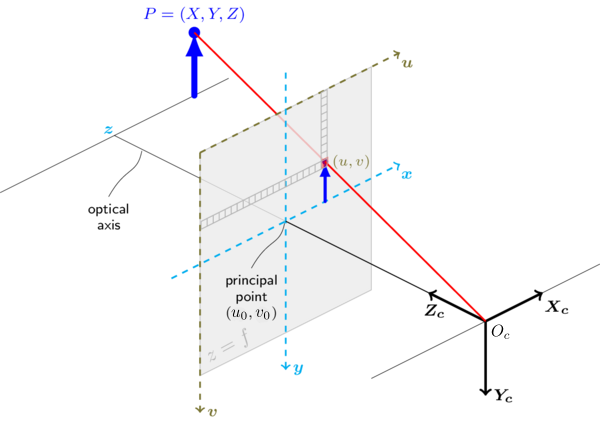
\includegraphics[width=0.8\linewidth]{./img/camera_model3.png}
\caption{Modelo da câmera (disponível em \citep{opencvCameraCalibration})}
\label{fig:camera_model}
\end{figure}

Em visão computacional geralmente é utilizado o modelo de perspectiva central mostrado na Figura \ref{fig:camera_model}.
Seja ${P} = [X\; Y\; Z]^T$ as coordenadas de um ponto expresso no sistema de coordenadas da câmera e ${p} = [x\;y]^T$ as coordenadas projetadas no plano da imagem por
% TODO confirmar referencial do mundo
\begin{equation}
x = f \frac{X}{Z}, \quad y = f \frac{Y}{Z}
\end{equation}

É possivel expressar o ponto no plano da imagem em coordenadas homogêneas na forma $\tilde{{p}} = [x'\; y' \; z']$ onde $x' = \frac{fX}{z'}$, $y' = \frac{fY}{z'}$ e $z' = Z$. Em forma matricial:

\begin{equation}
{\tilde{p}} = 
\m{ f & 0 & 0 \\
	 0 & f & 0 \\
	 0 & 0 & 1	
}
\m{X\\Y\\Z}
\end{equation}

Podemos retornar às coordenadas não-homogêneas com:
\[ x = \frac{x'}{z'} \qquad y = \frac{y'}{z'}\]

O ponto ${P}$ expresso no sistema de coordenadas inercial pode ser representado em coordenadas homogêneas como $({\tilde{P}})_C = [X \; Y \; Z \; 1]^T$ no referencial da câmera. A projeção de perspectiva é escrita em forma linear por 

\begin{equation} \label{eq:projpersp}
\tilde{{p}} = \m{
    f & 0 & 0 & 0 \\
    0 & f & 0 & 0 \\
    0 & 0 & 1 & 0
} (\tilde{{P}})_C
\end{equation}
A matriz pode ser fatorada como %ou $\tilde{p} = C (\tilde{{P}})_C$, onde $C$ é chamada de matriz da câmera. 
\begin{equation}
\tilde{{p}} = \m{
    f & 0 & 0 \\
    0 & f & 0 \\
    0 & 0 & 1 
} 
\m{
    1 & 0 & 0 & 0 \\
    0 & 1 & 0 & 0 \\
    0 & 0 & 1 & 0
}(\tilde{{P}})_C
\end{equation}
onde a primeira matriz é chamada de matriz da câmera e a segunda de matriz de projeção.

Uma imagem digital pode ser interpretada como uma matriz bidimensional de \textit{pixels}. As coordenadas de um ponto são expressas, portanto, em \textit{pixels} como um vetor de números inteiros $[u\; v]$. As coordenadas no plano da imagem se relacionam com as coordenadas em \textit{pixels} por
\begin{equation}
u =  \frac{x}{\rho_w} + u_0 \qquad v = \frac{y}{\rho_h} + v_0
\end{equation}
onde $\rho_w$ e $\rho_h$ são a largura e altura de cada \textit{pixel} respectivamente e $[u_0\;\; v_0]$ são as coordenadas do ponto em que o eixo ótico intercepta o plano da imagem.

Reescrevendo a equação \eqref{eq:projpersp} adicionando uma matriz ${K}$ de parâmetros

\begin{equation} \label{eq:camera_parameter}
{\tilde{p}_{px}} = 
\m {
	1/\rho_w & 0 & u_0 \\
	0        & 1/\rho_h &v_0 \\
	0 & 0 & 1 \\
}
\m{ f & 0 & 0 & 0\\
	 0 & f & 0 & 0\\
	 0 & 0 & 1 & 0	
}
(\tilde{{P}})_C
\end{equation}
onde $\tilde{p}_{px} = [u' \;\; v' \;\; w']$ são as coordenadas homogêneas em pixels do ponto $P$. As coodenadas não homogêneas no plano da imagem são dadas por
\begin{equation}
u = \frac{u'}{w'} \qquad v = \frac{v'}{w'}.
\end{equation} 
A câmera possui uma posição e orientação arbitrárias com respeito ao sistema de coordenadas inercial, logo a posição do ponto com respeito a câmera é dada por  $({\tilde{P}})_c = {T}_{0c}^{-1} {\tilde{P}}$. Utilizando a equação \eqref{eq:camera_parameter} podemos escrever a projeção da câmera na sua forma geral como
% TODO: confirmar
\begin{align}\label{eq:camera_projection}
{\tilde{p}_{px}} =& 
\m {
	f/\rho_w & 0 & u_0 \\
	0        & f/\rho_h &v_0 \\
	0 & 0 & 1 \\
}
\m{  1 & 0 & 0 & 0\\
	 0 & 1 & 0 & 0\\
	 0 & 0 & 1 & 0	
}
{T}_{0c}^{-1} (\tilde{{P})}_0\\
=& {K} {P}_0 {T}_{0c}^{-1} (\tilde{{P}})_0 \\ 
=& {C} ({\tilde{P})_0}
\end{align}

A equação \eqref{eq:camera_projection} expressa a posição de um ponto no plano da imagem em coordenadas homogêneas. A matriz $C$ realiza a mudança de escala, transformação e projeção de perspectiva. 

%\subsection{Calibração da Câmera}
%TODO

\subsection{Estimação da Pose}
O problema de estimar a \textit{pose} consiste em determinar a posição e orientação ${T}_{ct}$ do alvo com respeito ao sistema de coordenadas da câmera. Considera-se que a geometria do alvo é conhecida, isto é um conjunto de pontos característicos $[X_i \; Y_i \; Z_i]$ com $i \in [1\; \cdots \; N]$, assim como os parâmetros intrínsecos da câmera. A imagem capturada pela câmera é processada e as coordenadas no plano da imagem $p_{px} = [u_i\; v_i]$ são determinadas utilizando algoritmos de visão computacional. Esse problema é conhecido como \textit{Perspective-n-Point}.

Existem diversas abordagens para solucionar esse problema. Aqui será destacado o caso simples com 3 pontos e comentada a abordagem de \citep{dementhon1995model}  para N pontos pois esta foi utilizada na implementação desse projeto. Maiores detalhes sobre implementações disponíveis em código aberto podem ser encontradas no apêndice \ref{chap:pose_est}. 

\subsubsection{P3P: Estimação da \textit{pose} com 3 pontos}
Para entender o problema, considera-se o caso mais simples, com 3 pontos, já que, teoricamente como a \textit{pose} pode ser representada por 6 parâmetros independentes, três pontos seriam capazes de resolver o problema \citep{marchand2016pose}. Sejam ${P_i} = [X_i \; Y_i \; Z_i ]^T$ onde $i = 1 \dots 3$ três pontos com coordenadas representadas no referencial da câmera. 

Primeiramente, é feita uma estimativa da coordenada de profundidade $Z_i$ de cada ponto utilizando a lei dos cossenos no triângulo dado por ${C} {P}_i {P}_j$ onde ${C}$ é o ponto onde a câmera está posicionada. Para cada par de correspondências $P_i \leftrightarrow p_i$ e $P_j \leftrightarrow p_j$ podemos escrever \citep{quan1999linear} 
%A distâncias entre $\bm{P}_i$ e $\bm{P}_j$ e $\bm{P}_i$ e $\bm{P}_j$  é conhecida.
\begin{equation}
d_{ij}^2 = w_i^2 + w_j^2 -2 w_i w_j \cos \theta_{ij}
\end{equation}
onde $d_{ij} = ||{P}_i - {P}_j||$, $w_i = ||{P}_i - C||$ e $w_j = ||{P}_j - {C}||$. Cada restrição pode ser escrita como 
\begin{equation}
f_{ij}(w_i, w_j) = w_i^2 + w_j^2 - 2w_i w_j \cos \theta_{ij} - d_{ij}^2 = 0
\end{equation}
resultando no sistema
\begin{align*}
\begin{cases}
f_{12}(w_1, w_2) = 0 \\ 
f_{13}(w_1, w_3) = 0 \\ 
f_{23}(w_2, w_3) = 0
\end{cases}
\end{align*}

Este sistema possui 8 soluções, no entanto como não possui termos lineares as soluções ocorrem em 4 pares. É possível manipular as equações de modo a chegar em uma polinomial de oitavo grau em $w_1$ somente com termos pares, isto é, uma polinomial de quarto grau em $w = w_1^2$.
\begin{equation}
g(x) = a_5 w^4 + a_4 w^3 + a_3 w^2 + a_2 w + a_1 = 0
\end{equation}

Essa equação possui solução fechada e como $w_i > 0$, então $w_1 = \sqrt{q}$. Logo, $w_1$ e $w_2$ são determinados unicamente a partir de $w_1$. Para obter solução única é preciso adicionar um quarto ponto, o que gera um sistema com mais restrições do que incógnitas. Uma possível abordagem é resolver o problema para subconjuntos de três pontos e encontrar a solução comum. No entanto isso não aumenta a precisão do resultado e se houver ruido pode ser difícil encontrar a solução comum. 

Conhecidas as distâncias $w_i$ dos pontos do mundo à câmera, essas distâncias são convertidas em coordenadas tridimensionais centradas na câmera através de ${P'}_i = w_i {K}^{-1} {p}_i$, onde ${K}$ é a matriz de calibração da câmera. O último passo é determinar a orientação, uma transformação de similaridade pode ser obtida através de dois pares de pontos ${P'}_i \leftrightarrow {P}_i$. A solução pode ser obtida através de mínimos utilizando quatérnions. A partir da estimativa da rotação a obtenção da translação e da escala seguem trivialmente. 

Esse método auxilia na compreesão do problema, porém não é robusto e é pouco preciso, além de que os dados redundantes (quarto ponto) não aumentam a precisão do resultado. Portanto, outros algoritmos foram propostos.

\subsubsection{PNP: Estimação da \textit{pose} com N pontos}
Em \citep{dementhon1995model} é proposto combinar dois algoritmos. O primeiro \textit{POS (Pose from Orthography and Scaling)} aproxima a projeção de perspectiva com uma projeção ortográfica (e de escala) e encontra a matriz de rotação e o vetor de translação do objeto resolvendo um sistema linear. O segundo algoritmo \textit{POSIT (POS with ITerations)}, usa a \textit{pose} aproximada pelo \textit{POS} em um \textit{loop} para computar melhores projeções ortográficas (e de escala) dos pontos característicos. Então o \textit{POS} é aplicado a essas projeções, invés de às projeções da imagem original. O \textit{POSIT} converge para medidas precisas em poucas iterações e pode utilizar mais pontos para insensibilidade a erros de medição e ruido. 

Uma desvantagem do \textit{POSIT} é que ele não é diretamente aplicável a pontos coplanares \citep{marchand2016pose}. No entanto, em \citep{oberkampf1996iterative} uma extensão ao \textit{POSIT} foi proposta, resolvendo o problema para 4 ou mais pontos coplanares. 


%Considerando $N$ pontos $P_i$, cujas coordenadas homogêneas são dadas por $\tilde{P}_i = [X_i \;\; Y_i \;\; Z_i \;\; 1]$. Essas coordenadas

\subsection{Servovisão Baseada em Posição}
Em um sistema de servovisão baseado em posição a posição e orientação do alvo com respeito a câmera ${T}_{ct}$ é estimada. O problema de estimação da posição e orientação foi discutido acima e as implementações disponíveis em código aberto estão listadas no Apêndice \ref{chap:pose_est}. Como desejamos que alguma ferramenta no efetuador seja capaz de atingir o alvo, é preciso saber a posição e orientação do alvo em relação ao efetuador, dada por
\begin{equation}
T_{et} = T_{ec} T_{ct}.
\end{equation} 
Especifica-se uma posição desejada relativa ao sistema de coordenadas do alvo  ${T}_{e^*t}$ e deseja-se determinar o movimento necessário para mover a câmera para a posição desejada, que chamamos de ${T}_\Delta$.
\begin{align}
 {T}_{et} =  {T}_\Delta {T}_{e^*t} \\
 {T}_\Delta  =   {T}_{et} {T}_{e^*t}^{-1}
\end{align}

Com isso é possível aplicar uma estratégia de controle cinemático de posição no referencial do efetuador de modo a atingir a posição e orientação desejada. A lei de controle
\begin{equation} \label{eq:visionctrllaw}
%{u} = ({J}_a)_e^{-1}{K}_v[({x}_o)_e - ({x}_t)_e]
{u} = ({J}_a)_e^{-1}{K}_v x_\Delta
\end{equation}
é capaz de fazer ${x_\Delta}(t) \rightarrow 0$ quando $t \rightarrow \infty$ se $\dot{{x}}_t = 0$. Na Equação \eqref{eq:visionctrllaw}, $x_\Delta$ é obtido a partir de $T_\Delta$.

%Na Equação \eqref{eq:visionctrllaw}, ${x}_t$ é um vetor do espaço operacional representando a posição e orientação do alvo, ${T}_{ct}$. O vetor $x_o$ representa a posição e orientação ${T}_{c^*t}$ no espaço operacional, podendo ser interpretado como um \textit{offset} em relação ao alvo.

\section{Controle de Força}
\subsection{Problema de Rastreamento}
Considera-se o problema de controle cinemático de força, para um manipulador já em contato com uma superfície, assumindo que a força de contato pode ser medida com um sensor acoplado ao efetuador. 

Em \citep{leite2011servo} aplica-se o controle de força com base em uma abordagem de controle cinemático. O objetivo de controle é seguir uma força desejada variante no tempo ${f}_d(t) \in \mathbb{R}^3$ a partir da força de contato ${f} \in \mathbb{R}^3$ ao longo da superfície de restrição, medida com um sensor de força:
\begin{equation} \label{eq:problema_ctrl_forca}
{f} \rightarrow {f}_d(t), \qquad {e}_f = {f}_d(t) - {f} \rightarrow 0
\end{equation}

A força de contato pode ser modelada como uma mola linear, através da Lei de Hooke:
\begin{equation} \label{eq:hooke_mat}
{f} = -{K}_s ({p} - {d}_s)
\end{equation}
onde ${p} \in \mathbb{R}^3$ é a posição inicial do ponto de contato e ${d}_s \in \mathbb{R}^3$ é um ponto da superfície, ${K}_s = k_s I$ é a matriz de rigidez e $k_s > 0$ é o coeficiente de rigidez da superfície.

Derivando \eqref{eq:problema_ctrl_forca} e \eqref{eq:hooke_mat} em relação ao tempo com respeito ao tempo, a equação do erro de força $e_f \in \mathbb{R}^3$ é dada por $\dot{{e}}_f = \dot{{f}}_d + {K}_s \dot{{p}}$. Considerando uma lei de controle de força com ação \textit{feedforward} e proporcional
\begin{equation}
{\bar{u}}_f = -{K}_s^{-1} (\dot{{f}}_d + {K}_f {e}_f)
\end{equation}
onde ${K}_f = k_f {I}$, a dinâmica do erro é governada por
\begin{equation}
\dot{{e}}_f + {K}_f {e}_f = 0.
\end{equation}
Portanto escolhendo $k_f$ como uma constante positiva, o sistema em malha fechada é exponencialmente estável. 

\subsection{Problema de Regulação}
%Quando não está disponível o sinal $\dot{f}$ ou o mesmo é muito ruidoso é possível utilizar uma 

A estratégia de controle de força baseada em uma ação proporcional e integral tem sido o algoritmo mais utilizado devido a sua robustez com respeito ao atraso de tempo de medição e capacidade de remoção de perturbações de força \citep{wilfinger1994integral}. No problema de regulação, o uso de um controlador PI permite evitar instabilidade em uma possível perda de contato.

Considerando o problema de regular a força de contato medida $f$ para uma força desejada constante $f_d$ ao longo da superfície. 
\begin{equation} \label{eq:ef_reg}
f \rightarrow f_d, \qquad e_f = f - f_d \to 0
\end{equation}
Como em geral as medidas podem ser contaminadas por ruído utiliza-se um filtro de primeira ordem.
\begin{equation} \label{eq:efilter_reg}
\tau \dot{e}'_{f} = -e'_{f} + e_f 
\end{equation}
onde $e'_{f} \in \mathbb{R}^3$ é o erro de força filtrado e $\tau$ é a constante de tempo do filtro. 

Derivando \eqref{eq:hooke_mat}, \eqref{eq:ef_reg} e \eqref{eq:efilter_reg} com respeito ao tempo, a equação do erro de força é dada por 
\begin{equation}
\tau \ddot{e}'_{f} + \dot{e}'_f = {f}_d + K_s \bar{u}_f
\end{equation}
onde $\bar{u}_f \in \mathbb{R}^3$ é a lei de controle de posição $\bar{u}_p$ em
\begin{equation}
\bar{u} = \m{ \bar{u}_p \\ \bar{u}_o }
\end{equation}

Considerando $\bar{u}_p = \bar{u}_f$, utiliza-se uma lei de controle proporcional
\begin{equation} \label{eq:pi_force}
\bar{{u}}_f = -{K}_s^{-1} ({K}_f {e'}_f + {K}_i \int_0^t {e'}_f (\tau)d\tau),
\end{equation}
onde $K_f = k_f I$ e $K_i = k_i I$. Portanto a dinâmica do erro é governada por 
\begin{equation}
\tau \dddot{e}'_f + \ddot{e}'_f + k_f \dot{e}'_f + k_i e_f = 0
\end{equation}

Assim, deve-se escolher $k_f$ e $k_i$ como constantes positivas satisfazendo as condições de estabilidade estabelecidas pelo critério de establididade de \textit{Routh–Hurwitz}, ou seja, $k_f > k_i \tau$. Sob essas condições o sistema em malha fechada é exponencialmente estável.


\section{Controle Híbrido de Força e Posição}

É chamado de controle híbrido a estratégia que envolve o uso de restrições artificiais para especificar alvos do sistema e controlar somente as variáveis que não estão sujeitas às restrições naturais \citep{xaud2016doris}. Dessa forma as variáveis que não estão restritas pelo ambiente não são afetadas pela lei de controle.

Considerando que força e posição estão em sub-espaços de trabalho complementares é possível dividir o controle de força em duas malhas que não se interferem. Essa separação é feita pela matriz de seleção ${S}$. O controlador híbrido utiliza a matriz ${S}$ para dividir as malhas de  força e a posição  que atuam sobre o erro computado no sistema de coordenadas ${E}_s$ da superfície de restrição. A lei de controle híbrido é definida como:

\begin{equation} \label{eq:ctrl_law}
{u}_h = {u}_{hf} + {u}_{hp}
\end{equation}
onde $u_{hf}$ e $u_{hp}$ são os sinais de controle atuando sobre os subespaços de força e posição respectivamente. 

Suponha que deseja-se aplicar controle de posição em $x_s$, $y_s$ e controle de força em $z_s$, normal a superfície de contato. A matriz de seleção de força é definida como
\begin{equation}
S_f = \m{
    0 & 0 & 0 \\
    0 & 0 & 0 \\
    0 & 0 & 1 
}
\end{equation}
e cumpre o papel de cancelar os esforços de controle nos graus de liberdade complementares. A matriz de seleção de posição é complementar e pode ser definida como
\begin{equation}
S_p = (I - S_f) = \m{
    1 & 0 & 0 \\
    0 & 1 & 0 \\
    0 & 0 & 0 
}
\end{equation}

Se o manipulador está sendo controlado em seu referencial base, utilizando o Jacobiano geométrico, a equação \eqref{eq:ctrl_law} deve ser representada como 
\begin{equation}
({u}_h)_b = ({u}_{hf})_b + ({u}_{hp})_b
\end{equation}

Geralmente o erro de posição é definido como $(e_p)_b = (p_d)_b - (p_{be})_b$, enquanto que o erro de força é definido com respeito ao sistema de coordenadas do efetuador  $(e_f)_e = f_d - (f_{c})_e$. O controle de posição utiliza uma estratégia de controle proporcional com feedforward definida como:
\begin{equation}
(\bar{u}_p)_b = (\dot{p})_b + K_{p} (e_p)_b
\end{equation}
Para o sinal de controle de força é utilizada um controle proporcional integral cuja lei é dada por 
\begin{equation}
(\bar{u}_f)_e = K_{pf} (e_f)_e + K_{if} \int^{\tau}_0 (e_f(\tau))_e d\tau
\end{equation}
onde a parcela feedforward não é utilizada, já que considera-se apenas o problema de \textit{set-point}, para o qual $\dot{f}_d$. Como a matriz de seleção desacopla os subespaços de controle somente no referencial da superfície $\bar{E}_s$, os sinais de controle devem ser representados primeiramente nesse sistema de coordenadas, antes de serem operados po $S$ e, então, representados de volta no sistema de coordenadas da base.

\begin{align}
({u}_{hf})_b &= R_{bs} S_f R_{se} (\bar{u}_f)_e \\
({u}_{hp})_b &= R_{bs} S_p R_{sb} (\bar{u}_p)_b 
\end{align}
onde $R_{bs}$ é a matriz de rotação do sistema de coordenadas $\bar{E}_b$ da base para o da superfície $\bar{E}_s$,   $R_{se}$ é a matriz de rotação do sistema de coordenadas $\bar{E}_s$ da superfície para o sistema de coordenadas do efetuador $\bar{E}_e$ e $R_{sb} = R_{bs}^T$. 

O controle híbrido pode ser representado pelo diagrama de blocos da figura \ref{fig:hybrid_block}.

\begin{figure}[H]
  \centering
  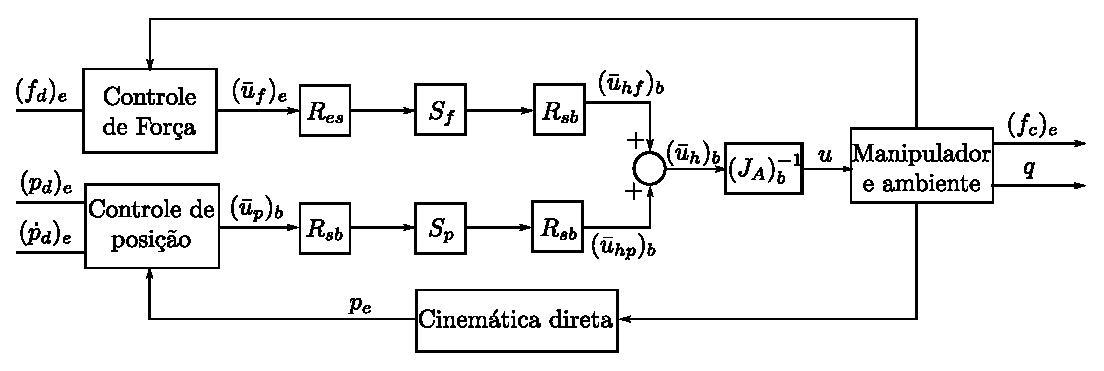
\includegraphics[width=\linewidth]{./img/hybrid.eps}
  \caption{Diagrama de blocos: Controle Híbrido Força-Posição}
  \label{fig:hybrid_block}
\end{figure}
  \chapter{TETIS - Modelagem e Controle}


\section{Modelo}
O manipulador TETIS consiste basicamente de um braço planar de três elos com uma rotação adicional ao redor do eixo do plano. Também pode ser visto como um braço antropomórfico com uma junta de revolução adicional ao final da cadeia, com o eixo paralelo às duas anteriores. O projeto mecânico faz com que a extremidade do efetuador final não esteja exatamente alinhada com as juntas, o que é levado em conta no último elo. O esquema na figura \ref{fig:modelo_tetis} ilustra o modelo de elos e juntas. 
\begin{figure}[!ht]
\centering
  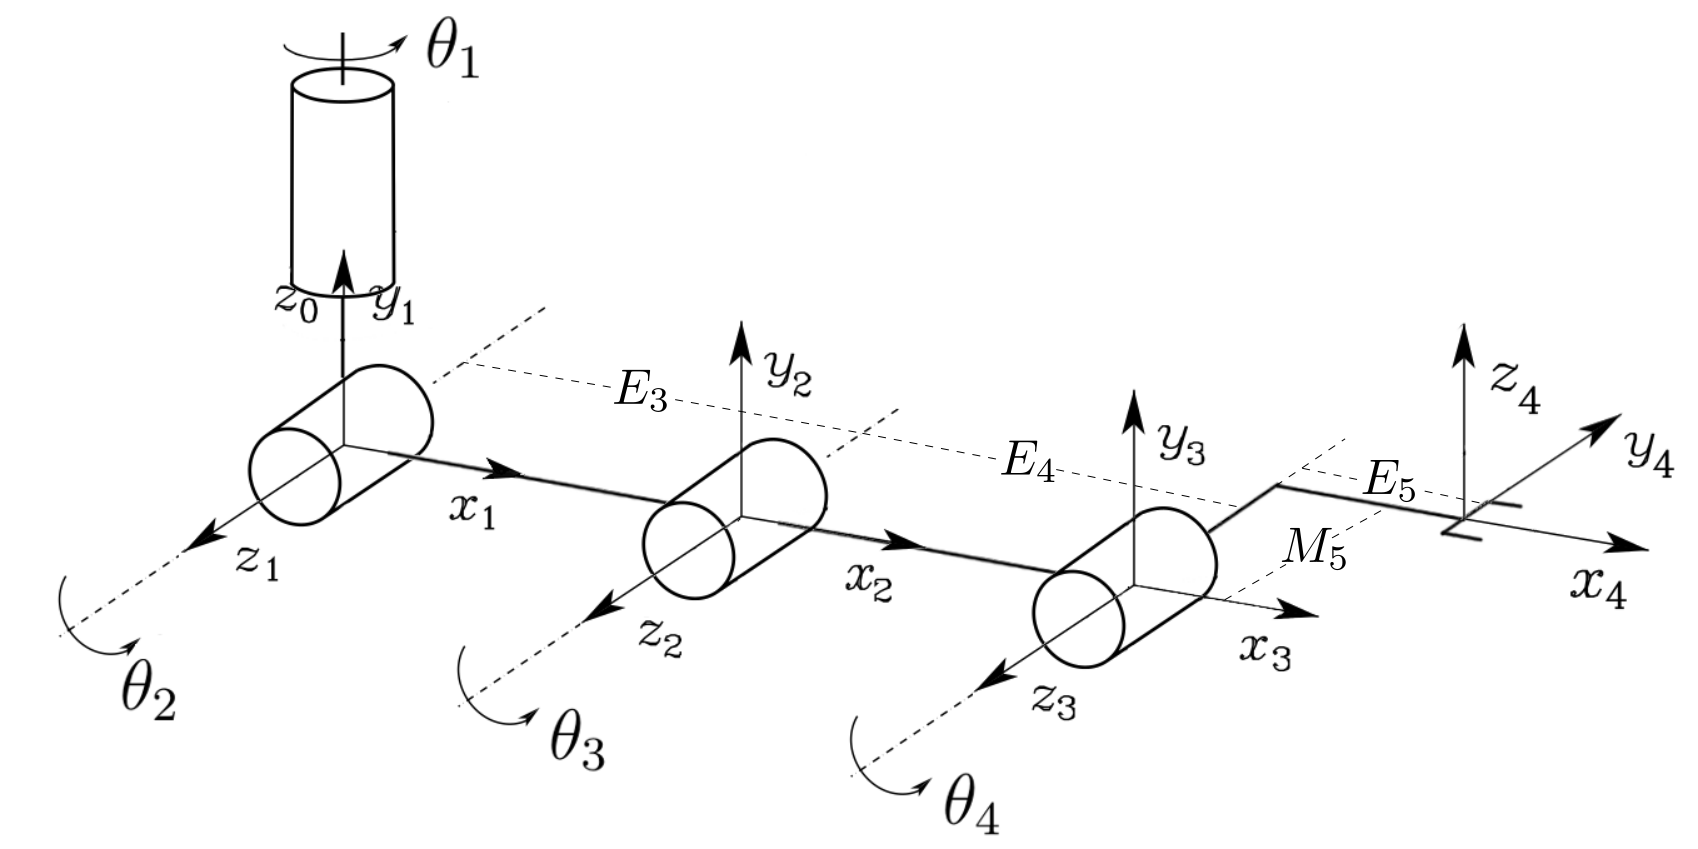
\includegraphics[width=0.9\linewidth]{./img/model3.png}
  \caption{Modelagem cinemática do manipulador TETIS e posicionamento dos sistemas de coordenadas}
  \label{fig:modelo_tetis}
\end{figure}%

\section{Cinemática Direta}
O primeiro passo ao modelar um manipulador robótico é encontrar a cinemática direta. Será utilizada a convenção de Denavit-Hartenberg para posicionar os sistemas de coordenadas e obter os parâmetros. Seguindo os passos descritos na Seção \ref{sec:denavit} os sistemas de coordenadas foram posicionados da seguinte forma:

\begin{itemize}
\item Eixo $\vec{z}_0$ escolhido ao longo da Junta 1. Origem $O_0$ escolhida arbitrariamente de modo a coincidir com $O_1$ por simplicidade.  
\item Eixo $\vec{z}_1$ escolhido ao longo da Junta 2. Origem $O_1$ na intersecção entre $\vec{z}_0$ e $\vec{z}_1$. Eixo $\vec{x}_1$ na direção normal ao plano definido por $\vec{z}_0$ e $\vec{z}_1$ pois se interceptam. O sentido foi arbitrariamente escolhido na direção de avanço da cadeia por simplicidade.
\item Eixo $\vec{z}_2$ escolhido ao longo da Junta 3. Origem $O_2$ na junta 3 pois $\vec{z}_2$ e $\vec{z}_1$ são paralelas. Eixo $\vec{x}_2$ escolhido arbitrariamente ao longo de $\vec{x}_1$ pois a normal comum entre $\vec{z}_2$ e $\vec{z}_1$ não é unicamente definida.
\item Eixo $\vec{z}_3$ escolhido ao longo da Junta 4. Origem $O_3$ na junta 3 pois $\vec{z}_3$ e $\vec{z}_2$ são paralelas. Eixo $\vec{x}_3$ escolhido arbitrariamente ao longo de  $\vec{x}_2$ pois a normal comum entre $\vec{z}_3$ e $\vec{z}_2$ não é unicamente definida.
\item Como não existe junta 5, eixo $\vec{z}_4$ definido arbitrariamente. Origem $O_4$ na extremidade do efetuador final. Eixo $\vec{x}_4$ normal ao eixo $\vec{z}_3$.
\end{itemize}

A partir dos eixos posicionados conforme a figura \ref{fig:modelo_tetis} é possível obter os parâmetros na tabela \ref{tab:dh_tetis}. 


\begin{table}[h!]
\centering
\caption{Parâmetros Denavit–Hartenberg para manipulador Tetis}
\label{tab:dh_tetis}
\begin{tabular}{rrrrr} \hline
Elo & $a_i$ & $\alpha_i$ & $d_i$  & $\theta_i$ \\ \hline
1   & 0     & $\pi/2$    & 0      & $\theta_1$ \\
2   & $E_3$ & 0          & 0      & $\theta_2$ \\
3   & $E_4$ & 0          & 0      & $\theta_3$ \\
4   & $E_5$ & $-\pi/2$   & $-M_5$ & $\theta_4$ \\ \hline
\end{tabular}
\end{table}


\begin{itemize}
\item $a_1 = 0$  e $d_1 = 0$ pois $O_0$ e $O_1$ coincidem. $\alpha_1 = \pi/2$ ângulo entre $\vec{z}_0$ e $\vec{z}_1$ ao redor de $\vec{x}_1$.
\item $a_2 = E_3$ é a distância entre $\vec{z}_1$ e $\vec{z}_2$ ao longo de $\vec{x}_2$ que corresponde ao comprimento do elo 2. $\vec{z}_1$ e $\vec{z}_2$ são sempre paralelos logo $\alpha_2 = 0$. A distância $d_2$ entre $\vec{x}_1$ e $\vec{x}_2$ ao longo de $\vec{z}_1$ é zero. 

\item $a_3 = E_4$ é a distância entre $\vec{z}_2$ e $\vec{z}_3$ ao longo de $\vec{x}_3$ que corresponde ao comprimento do elo 3. $\vec{z}_2$ e $\vec{z}_3$ são sempre paralelos logo $\alpha_3 = 0$. A distância $d_3$ entre $\vec{x}_2$ e $\vec{x}_3$ ao longo de $z_2$ é zero. 

\item $a_4 = E_5$ é a distância entre $\vec{z}_3$ e $\vec{z}_4$ ao longo de $\vec{x}_4$. $\alpha_4 = -\pi/2$ é o ângulo entre $\vec{z}_3$ e $\vec{z}_4$ ao redor de $\vec{x}_4$, sendo portanto negativo. $d_4 = -M_5$ é a distância entre $\vec{x}_3$ e $\vec{x}_4$ ao longo de $\vec{z}_3$. 
\end{itemize}

Considerando a posição inicial da figura \ref{fig:modelo_tetis} todos os ângulos $\theta_i$ são dados diretamente pelas variáveis de junta, sem \textit{offsets}. 


Obtemos a partir da equação \eqref{eq:transform_dh} as transformações homogêneas entre sistemas de coordenadas consecutivos:
%\begin{align*}
%\bm{R}_{01} =
%\m{c_1 & 0 & s_1   \\
%   s_1 & 0 & -c_1  \\
%   0   & 1 &    0  \\} 
%& & \vec{\bm{p}}_{01} = 0
%\end{align*}
%\begin{align*}
%R_{12} = 
%\m{c_2 & -s_2 &  0  \\
%   s_2 &  c_2 &  0  \\
%   0   &    0 &  1  \\} 
%\end{align*}
%\begin{align*}
%R_{23} = 
%\m{c_3 & -s_3 &  0  \\
%   s_3 &  c_3 &  0  \\
%   0   &    0 &  1  \\} 
%\end{align*}
%\begin{align*}
%R_{34} = 
%\m{c_4 &  0 & -s_4  \\
%   s_4 &  0 &  c_4  \\
%   0   & -1 &    0  \\} 
%\end{align*}


%\begin{equation}
%\bm{R}_{04} = 
%\m{
%	c_1 c_{234} & -s_1 & -c_1 s_{234} \\
%	s_1 c_{234} & -c_1 & -s_1 s_{234} \\
%		s_{234} &    0 & 	  c_{234}
%}
%\end{equation}

\begin{align*}
{T}_{01} = 
\m{c_1 & 0 & s_1 &  0 \\
   s_1 & 0 & -c_1 & 0 \\
   0   & 1 &    0 & 0 \\
   0   & 0 &    0 & 1}
& &
{T}_{12} =  \m{c_2 & -s_2 &  0 & E_3 c_2 \\
   s_2 &  c_2 &  0 & E_3 s_2  \\
   0   &    0 &  1 & 	   0  \\
   0   &    0 &  0 &       1} 
\end{align*}

\begin{align*}
{T}_{23} = 
\m{c_3 & -s_3 &  0 & E_4 c_3 \\
   s_3 &  c_3 &  0 & E_4 s_3  \\
   0   &    0 &  1 & 	   0  \\
   0   &    0 &  0 &       1}
& &
{T}_{34} = 
\m{c_4 &    0 &  -s_4 & E_5 c_4 \\
   s_4 &    0 &   c_4 & E_5 s_4 \\
   0   &   -1 &     0 & 	-M_5 \\
   0   &    0 &     0 &       1}
\end{align*}


\begin{equation} \label{eq:cine_direta}
{T}_{04} = {T}_{01} {T}_{12}  {T}_{23} {T}_{34} = 
\m{
   c_1 c_{234} & -s_1 & -c_1 s_{234} & -M_5 s_1 + E_4 c_{23}c_1 + E_3 c_1 c_2 + E_5 c_{234} c_1 \\
   s_1 c_{234} & -c_1 & -s_1 s_{234} &   M_5 c_1+E_4 c_{23} s_1 + E_3 c_2 s_1 + E_5 c_{234} s_1 \\
   s_{234}     &    0 &      c_{234} &					     E_4 s_{23} + E_3 s_2 + E_5 s_{234} \\
   0   &    0 &     0 &      												   1
} 
\end{equation}

Definindo ${T}_{b0} = {I}$ e ${T}_{4e} = {I}$, pela equação \eqref{eq:base_efetuador} temos
\begin{equation}
{T}_{be} ({q}) = {T}_{04}({q})
\end{equation}


\section{Espaço das Juntas e Operacional}
Antes de tratar de estratégias de controle é necessário definir o espaço operacional e o espaço das juntas,  sob os quais serão aplicadas as leis de controle. 
Como trata-se de um manipulador 4-DOF de temos que o vetor do espaço operacional tem dimensão $(4 \times 1)$ dado por 
\begin{equation} \label{eq:operational_space}
{x_e} = \m{{p}_{be} \\ \phi_{be}}
\end{equation}
onde o vetor $p_{be}$ descreve a posição cartesiana representada no referencial da base e $\phi_{be}$ é o grau de liberdade de orientação \textit{pitch}, dado por
\begin{equation} \label{eq:orientacao}
\phi_{be} = -(\theta_2 + \theta_3 + \theta_4)
\end{equation}

O espaço das juntas é definido por 
\begin{equation} \label{joint_space}
{q} = \m{q_1 \\ q_2 \\ q_3 \\ q_4} = \m{\theta_1 \\ \theta_2 \\ \theta_3 \\ \theta_4  }
\end{equation} 
pois todas as juntas são de revolução.

\section{Cinemática Diferencial}

\subsection{Jacobiano Analítico}
A partir da cinemática direta em \eqref{eq:cine_direta} e da equação \ref{eq:jacob_pos} podemos obter o Jacobiano de posição para o manipulador diferenciando a equação em relação as variáveis de junta. 
\begin{equation}
{p}_{be} = \m{p_{be_x} \\ p_{be_y} \\ p_{be_z}} =
\m{
   -M_5 s_1 + E_4 c_{23}c_1 + E_3 c_1 c_2 + E_5 c_{234} c_1 \\
     M_5 c_1+E_4 c_{23} s_1 + E_3 c_2 s_1 + E_5 c_{234} s_1 \\
   						 E_4 s_{23} + E_3 s_2 + E_5 s_{234} \\
}
\end{equation}

\begin{equation}
({J}_{ap})_b = 
\m{
	\ddfrac{\partial x}{\partial q_1} & \ddfrac{\partial x}{\partial q_2} & \ddfrac{\partial x}{\partial q_3} & \ddfrac{\partial x}{\partial q_4}  \\
	\ddfrac{\partial y}{\partial q_1} & \ddfrac{\partial y}{\partial q_2} & \ddfrac{\partial y}{\partial q_3} & \ddfrac{\partial y}{\partial q_4}  \\
	\ddfrac{\partial z}{\partial q_1} & \ddfrac{\partial z}{\partial q_2} & \ddfrac{\partial z}{\partial q_3} & \ddfrac{\partial z}{\partial q_4}  \\
}
\end{equation}
onde
\allowdisplaybreaks
\begin{align*}
&\frac{\partial x}{\partial q_1} =& - M_5c_1 - E_4c_{23}s_1 - E_3c_2s_1 - E_5c_{234}s_1  \\
&\frac{\partial x}{\partial q_2} =& -c_1(E_4s_{23}+E_3s_2+E_5s_{234}) \\
&\frac{\partial x}{\partial q_3} =& -c_1(E_4s_{23}+E_5s_{234}) \\
&\frac{\partial x}{\partial q_4} =& -E_5s_{234}c_1 \\
&\frac{\partial y}{\partial q_1} =& -M_5s_1+E_4c_{23}c_1+E_3c_1c_2+E_5c_{234}c_1 \\
&\frac{\partial y}{\partial q_2} =& -s_1(E_4s_{23}+E_3s_2+E_5s_{234}) \\
&\frac{\partial y}{\partial q_3} =& -s_1(E_4s_{23}+E_5s_{234}) \\
&\frac{\partial y}{\partial q_4} =& -E_5s_{234}s_1 \\ 
&\frac{\partial z}{\partial q_1} =& 0 \\ 
&\frac{\partial z}{\partial q_2} =& E_4c_{23}+E_3c_2+E_5c_{234} \\
&\frac{\partial z}{\partial q_3} =& E_4c_{23}+E_5c_{234}\\
&\frac{\partial z}{\partial q_4} =& E_{5}c_{234} 
\end{align*}

A partir de \ref{eq:jacob_or} e de \ref{eq:orientacao} podemos calcular o Jacobiano de orientação
\begin{equation}
{J}_{a\phi}({q}) = \frac{\partial \phi_e}{\partial {q}} = \m{0 & -1 & -1 & -1}
\end{equation}
 
Em alguns modos como controle por servovisão e no controle manual com \textit{joystick} é interessante fazer o controle no referencial do efetuador, portanto precisamos representar o Jacobiano de posição no referencial do efetuador como $({J}_{ap})_e = {R}_{be}^T ({J}_{ap})_b$.  

\begin{equation}
({J}_{ap})_e =  
\m{
    -M_5c_{234} & E_3s_{34}+E_4s_4 & E_4s_4 & 0 \\
    E_4c_{23}+E_3c_2+E_5c_{234} & 0 & 0 & 0 \\
    M_5s_{23} &  E_5+E_3c_{34}+E_4c_4 & E_5+E_4c_4 & E_5 
}
\end{equation}

Note que para a escolha de sistemas de coordenadas do TETIS tem-se que
\begin{equation}
(J_{a\phi})_e = (J_{a\phi})_b.
\end{equation}
%A partir daqui, para simplificar a notação, sempre será referenciado o Jacobiano Analitico no referencial da base $(\bm{J}_A)_0$  como  $\bm{J}_0$ e o Jacobiano Analítico no referencial do efetuador $(\bm{J}_A)_N$ como $\bm{J}_N$.

%\section{Singularidades}

\section{Malha Aberta no Espaço Operacional} 
Este é um modo em malha aberta, onde o sinal de entrada no controlador é de velocidade no referencial da base ou do efetuador, ou seja a velocidade linear ${\dot{p}}_d$. Utiliza-se a equação \eqref{eq:jacob_pos} para calcular a velocidade de cada junta. 

\begin{figure}[h!]
\centering
\begin{tikzpicture}[auto, node distance=2cm,>=latex']
    % We start by placing the blocks
    \node [input, name=input] {};
    \node [block, right of=input] (J) {$J_a^{-1}$};
    \node [block, right of=J] (Integral) {$\int$};
    \node [output, right of=Integral] (output) {};

    \draw [draw,->] (input) -- node {$\dot{{x}}_d$} (J);
    \draw [->] (J) -- node {${\dot{q}}$} (Integral);
    \draw [->] (Integral) -- node [name=x] {${q}$}(output);
\end{tikzpicture}
\caption{Diagrama de Blocos: Modo de velocidade do Espaço Operacional}
\label{fig:vel_op}
\end{figure}


\subsection{Sistema de coordenadas da Base} \label{sec:openloopbase}
Quando o controle é feito no referencial da base $({\dot{x}}_d)_b$ é velocidade desejada expressa no referencial da base e utiliza-se $({J}_{a})_b$.
\begin{equation}
{u} = {\dot{q}}_d = ({J}_{a})_b^{-1} ({\dot{x}}_d)_b
\end{equation}
\subsection{Sistema de coordenadas do Efetuador} \label{sec:openloopefct}
Quando o controle é feito no referencial do efetuador $({\dot{x}}_d)_e$ é velocidade desejada expressa no referencial do efetuador e utiliza-se $({J}_{a})_e$.
\begin{equation}
{u} = {\dot{q}}_d = ({J}_{a})_e^{-1} ({\dot{x}}_d)_e
\end{equation}
onde 
\begin{equation}
{\dot{x}}_d = \m{{\dot{p}}_d \\ \dot{\phi}_d}
\end{equation}

\section{Controle de Posição no Espaço das Juntas} \label{sec:position_joint}
O controle de posição no espaço das juntas consiste em uma realimentação com controle proporcional individual para cada junta. Considerando que as juntas sejam modeladas como integradores, o diagrama \ref{fig:pos_juntas} mostra a malha de controle.

\begin{figure}[h!]
\centering
\begin{tikzpicture}[auto, node distance=2cm,>=latex']
    % We start by placing the blocks
    \node [input, name=input] {};
    \node [sum, right of=input] (sum) {};
    \node [block, right of=sum] (controller) {${K}_j$};
    \node [block, right of=controller] (system) {$\ddfrac{1}{s}$};
    % We draw an edge between the controller and system block to 
    % calculate the coordinate u. We need it to place the measurement block. 
    \draw [->] (controller) -- node[name=u] {${u}$} (system);
    \node [output, right of=system] (output) {};
    \node [tmp, below of=u] (tmp1) {};

    % Once the nodes are placed, connecting them is easy. 
    \draw [->] (system) -- node [name=s] {${q}$}(output);
    \draw [draw,->] (input) -- node {${q_d}$} (sum);
    \draw [->] (sum) -- node {${e}$} (controller);
    \draw [->] (s) |- (tmp1)-| node[pos=0.99] {$-$} node [near end] {${q}$} (sum);
       %\draw [->] (measurements) -| node[pos=0.99] {$-$} 
       % node [near end] {$\bm{q}_m$} (sum);
\end{tikzpicture}
\caption{Diagrama de Blocos: Modo de Posição no Espaço das Juntas}
\label{fig:pos_juntas}
\end{figure}

A lei de controle é dada por 
\begin{equation}
{u} = {K}_j ({q}_d - {q})
\end{equation}
onde ${K_j} = k_j {I} > 0$.

\section{Controle de Posição no Espaço Operacional} \label{sec:pos_operacional}
Para este modo considera-se o problema de \textit{set-point} para o controle de posição no espaço operacional conforme definido em \ref{eq:op_space}. Para referências constantes, ou seja, quando $\dot{{x}}_d = 0$ a lei de controle dada por
\begin{equation} \label{eq:lei_posicao}
{u} = ({J}_{a})_b^{-1} {K}_p ( {x_d} - ({x_{be}})_b)
\end{equation}
é capaz de levar o ${e} \rightarrow 0$ quando $t \rightarrow \infty$.

\section{Controle Proporcional com Feedforward} \label{sec:pplusf}
Para o rastreamento de trajetória considera-se o problema de seguir um referência no referencial da base ${x}_d(t)$ que é função do tempo, conhecidos ${x}_d(t)$ e ${\dot{x}}_d(t)$. Para levar o erro assintoticamente a zero, utiliza-se uma lei de controle proporcional com \textit{feedforward} utilizando a inversa do Jacobiano Analítico. Conforme mostrado na Seção \ref{sec:controle_cinematico}, a lei de controle dada por 
\begin{equation}
{u} = ({J}_{a})_b^{-1} [\dot{{x}}_d + {K}_t ({x_d} - (x_{be})_b)]
\end{equation} 
é capaz de levar o erro assintoticamente a zero pois a dinâmica fica 
\begin{equation}
\dot{{e}} + {K} {e} = 0
\end{equation}
O algoritmo de controle pode ser resumido por:
\begin{align}
{e} &= {x}_d- (x_{be})_b  \label{eq:error_pf}\\
{\bar{u}} &= {K}_t {e} + ({\dot{x}}_d)_b \\
{u} &= ({J}_a)_b^{-1} {\bar{u}}
\end{align}

%\begin{algorithm}
%\caption{<your caption for this algorithm>}
%\begin{algorithmic}
%\State $t = getTime()$
%\State $t = getTime()$
%\If {$i\geq maxval$}
%%    \State $i\gets 0$
%\Else
%    \If {$i+k\leq maxval$}
%        \State $i\gets i+k$
%    \EndIf
%\EndIf
%\end{algorithmic}
%\end{algorithm}

\section{Controle por Servovisão} \label{sec:servo_vision}
O controle por servovisão no manipulador TETIS é feito através de uma configuração \textit{eye-in-hand}, onde a câmera é montada no efetuador final do manipulador, utilizando a abordagem de Servovisão Baseada em Posição (PBVS). Na Seção \ref{sec:minoru} é descrita a câmera utilizada. Trata-se de uma câmera estereoscópica, no entanto será utilizada apenas um dos sensores. Assume-se que é possível aproximar a câmera pelo modelo \textit{pin-hole} descrito na Seção \ref{sec:camera_model}. Consideram-se desprezíveis as distorções geométricas causadas pelas lentes.

%\begin{figure}[H]
%\centering
%\begin{subfigure}{.5\textwidth}
%  \centering
%  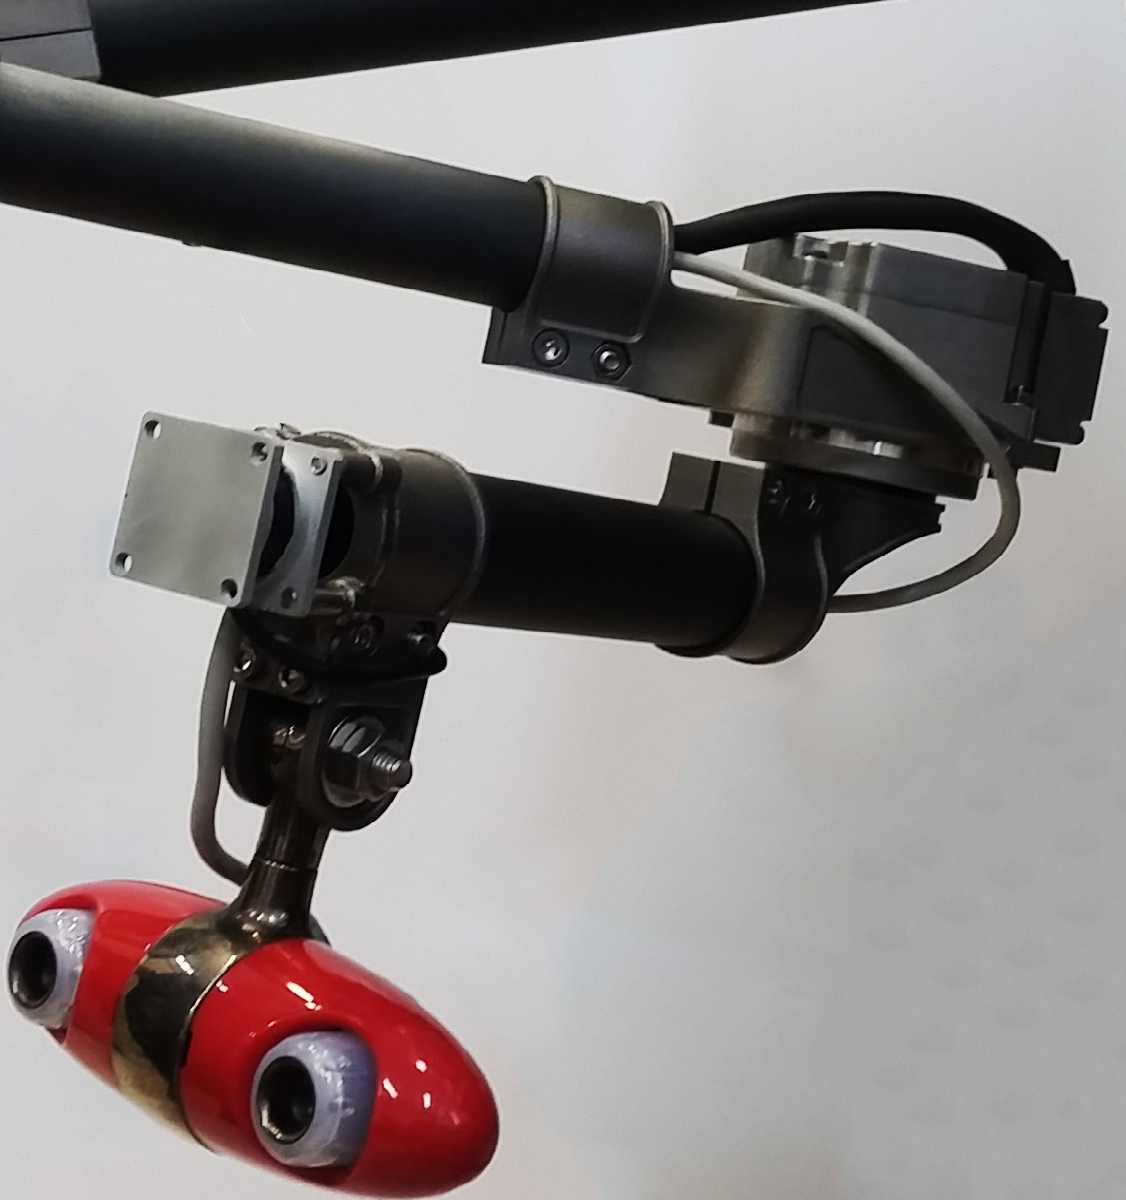
\includegraphics[width=\linewidth]{./img/manip_zoom.png}
%  \caption{Efetuador com câmera}
%  \label{fig:efetuador}
%\end{subfigure}%
%\begin{subfigure}{.5\textwidth}
%  \centering
%  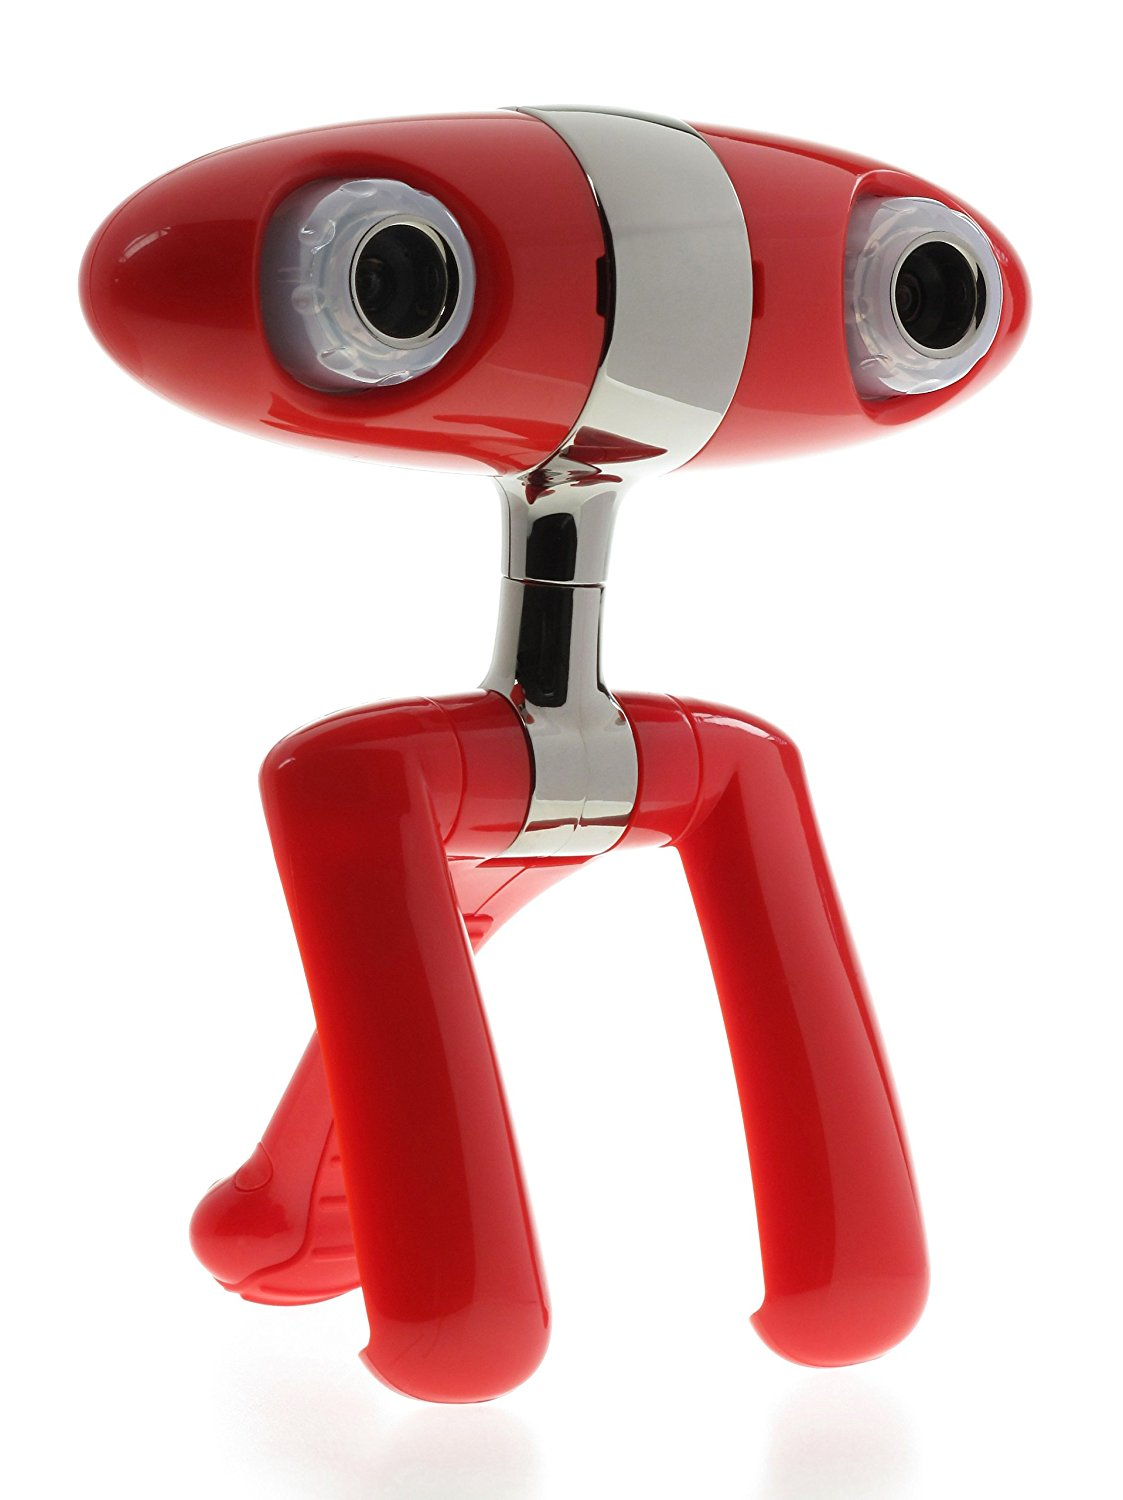
\includegraphics[width=0.8\linewidth]{./img/minoru.jpg}
%  \caption{Minoru Camera}
%  \label{fig:minoru}
%\end{subfigure}
%\label{fig:efet_minoru}
%\caption{Efetuador e câmera Minoru}
%\end{figure}


O objetivo é deste modo de controle é rastrear um alvo, que é representado por um QR code como o da Figura \ref{fig:camera_target}. Deseja-se que o efetuador rastreie sempre a orientação normal ao plano do alvo.

A matriz de calibração ${K}$ da equação \eqref{eq:camera_projection} obtida através do processo descrito em \citep{visp_camera_calibration} é:

\begin{equation}
{K} = \m {
	f/\rho_w & 0 & u_0 \\
	0        & f/\rho_h &v_0 \\
	0 & 0 & 1 \\
}
=
\m{
	877.62 	& 0 		& 306.53 \\
	0  		& 880.32 	& 210.12 \\
	0   	& 0 		& 1 \\	
}	
\end{equation}

Observando que o referencial da câmera e do efetuador são dados pela Figura \ref{fig:camera_ref}, podemos chegar a seguinte transformação homogênea

\begin{equation} \label{eq:tec}
{T}_{ec} = \m{
	0 & 0 & 1 & -30 \\
	0 & -1 & 0 & 101 \\
	1 &  0 & 0 & -43 \\
	0 &  0 & 0 &  1
}
\end{equation}

\begin{figure}[!h]
  \centering
  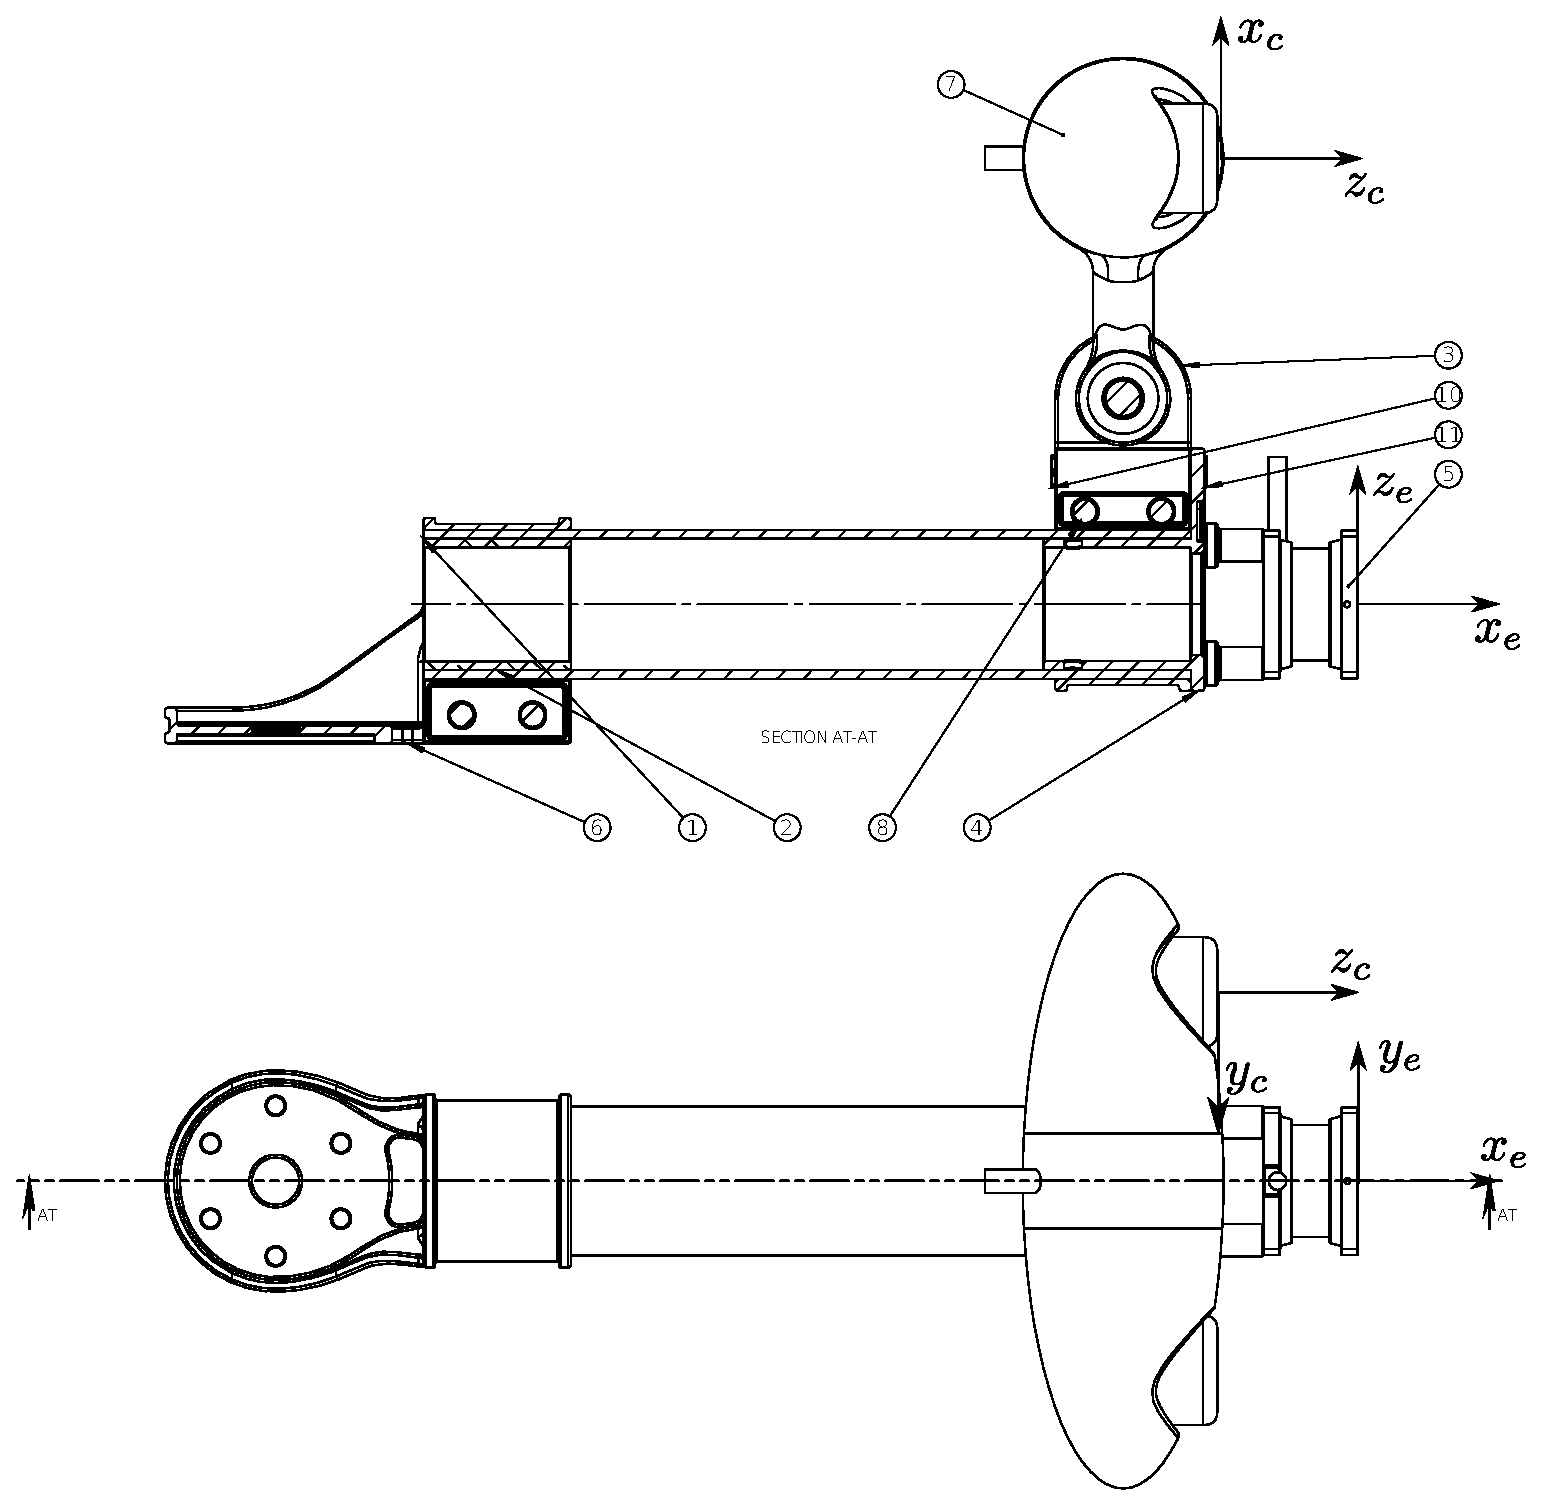
\includegraphics[width=0.8\linewidth]{./img/effector2}
  \caption{Sistemas de coordenadas da câmera e do efetuador}
  \label{fig:camera_ref}
\end{figure}

\begin{figure}[!h]
  \centering
  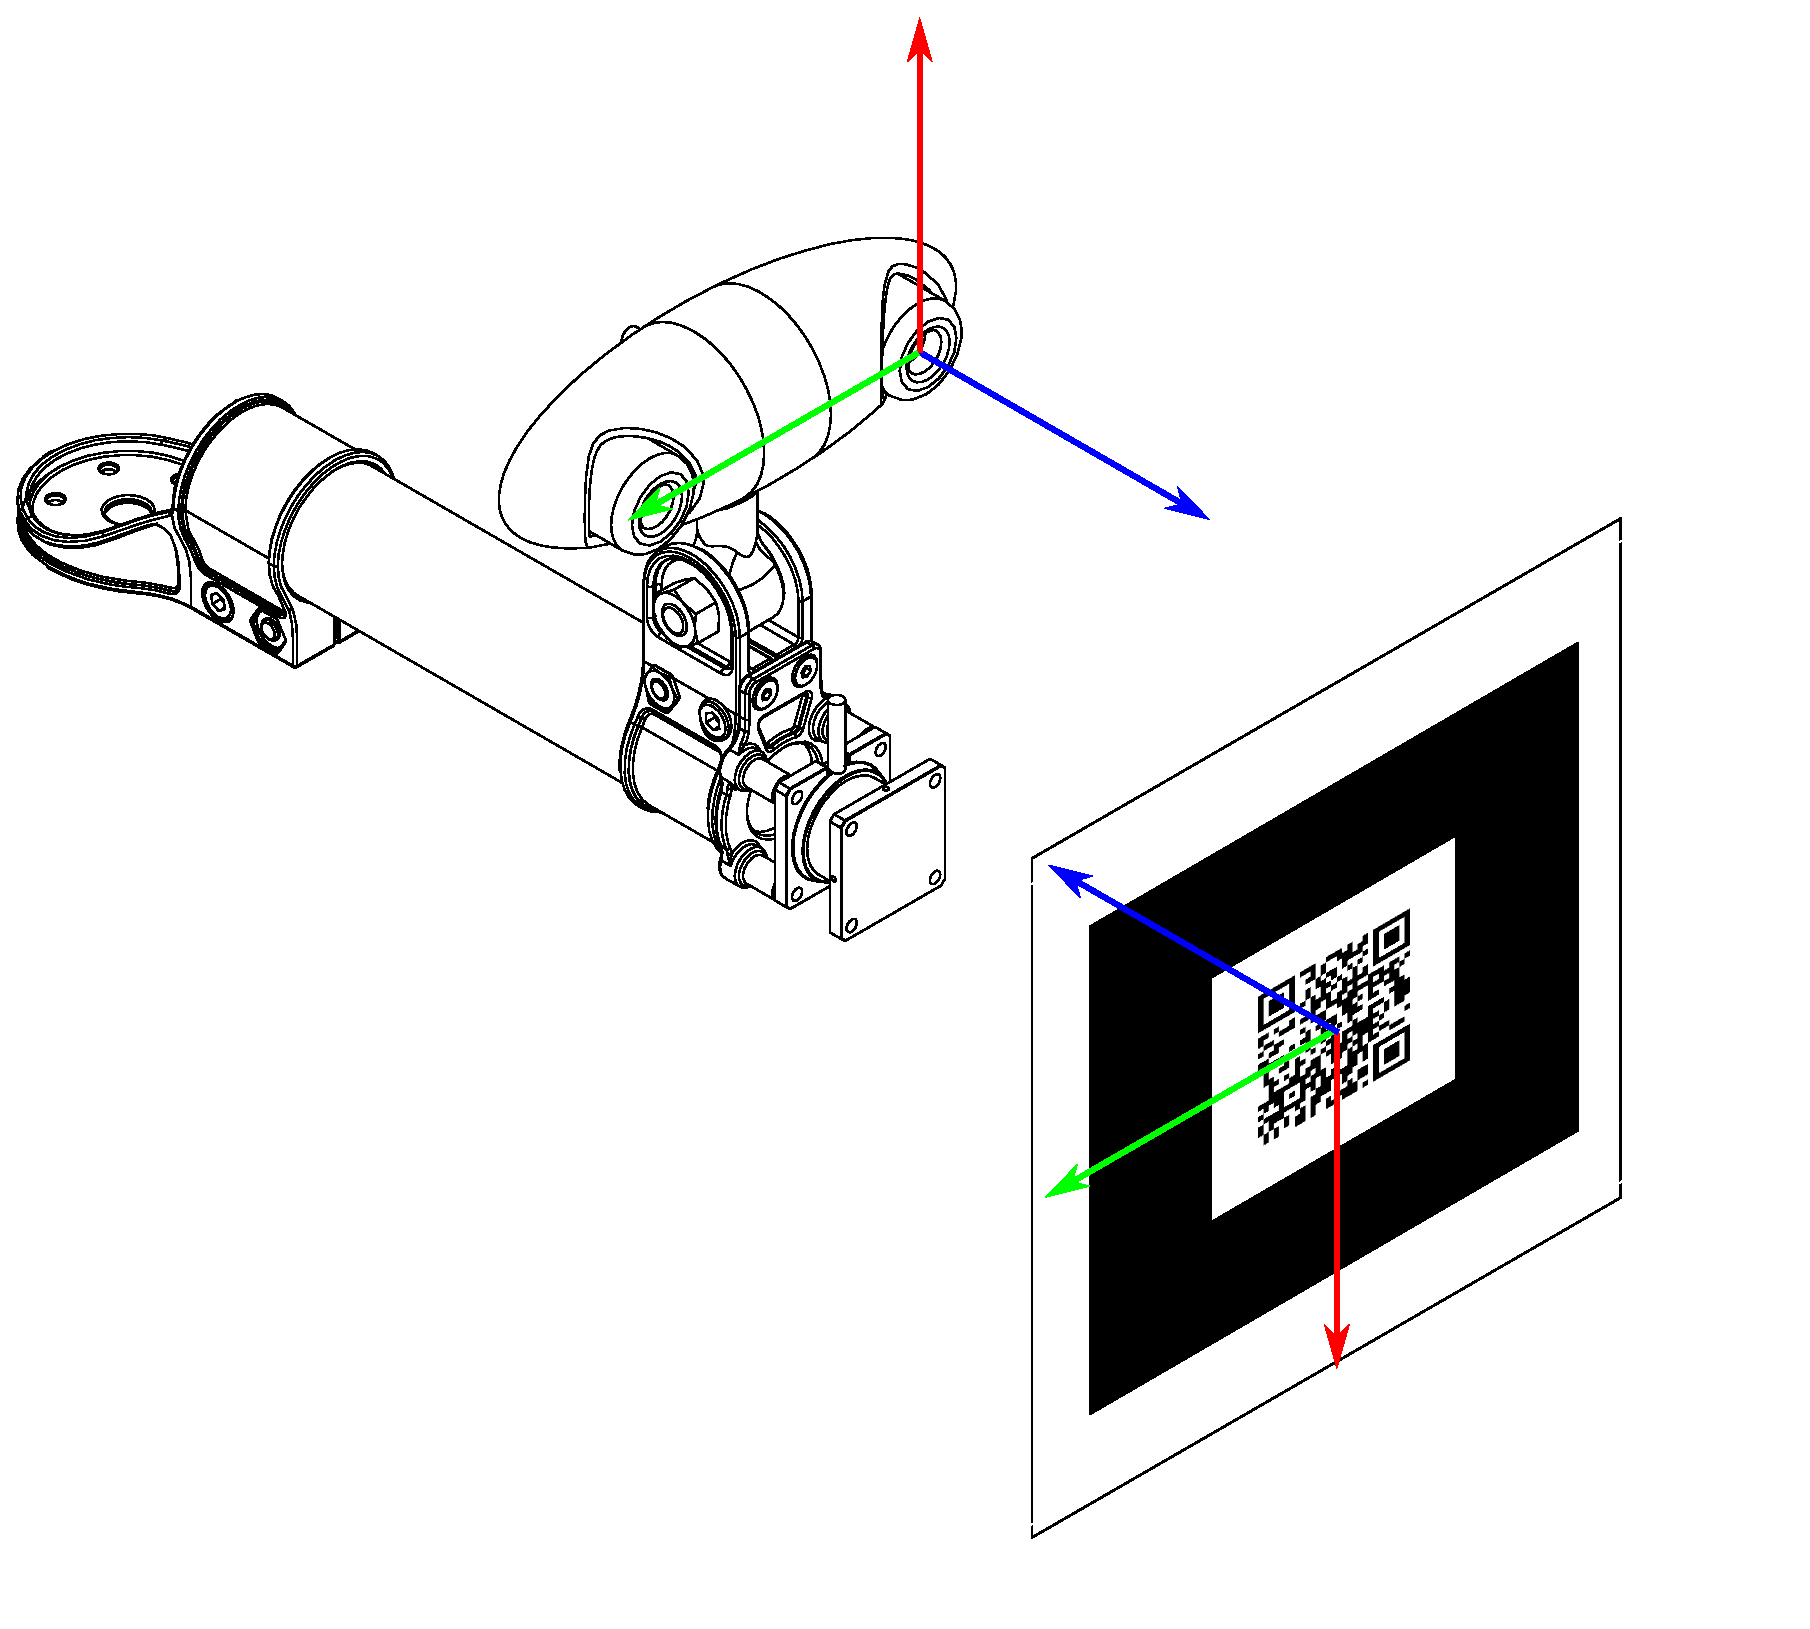
\includegraphics[width=0.8\linewidth]{./img/camera_target}
  \caption{Sistemas de coordenadas da câmera e do alvo}
  \label{fig:camera_target}
\end{figure}


Para a abordagem PBVS, foi utilizada a lei de controle proporcional descrita na equação \eqref{eq:visionctrllaw}
\begin{equation*} 
{u} = ({J}_a)_e^{-1}{K}_v x_\Delta%[({x}_o)_e - ({x}_t)_e]
%{u} = ({J}_{a})_e^{-1} {K}_t [({x}_t)_e - ({x_e})_e]
\end{equation*}
onde $x_\Delta = ({x}_{et})_e - ({x}_{e^*t})_e$. O vetor do espaço operacional ${x}_{e^*t}$ representa uma posição e orientação relativa ao alvo, enquanto que $({x}_{et})_e$ é obtida a partir de $T_{et}$.
%onde ${x}_o$ e ${x_t}$ estão representados no referencial do efetuador. Portanto precisamos saber a posição e orientação ${x}_t$ do alvo em relação ao efetuador

\begin{equation}
{T}_{et} = {T}_{ec} {T}_{ct}
\end{equation}
onde ${T}_{ec}$ é dado por \eqref{eq:tec} e ${T}_{ct}$ obtemos através de algoritmos de estimação de posição e orientação a partir de visão computacional. Ficamos então com

\begin{equation}
({x}_{et})_e = \m{ ({p}_{et})_e \\ (\phi_{et})_e }
\end{equation}
onde $({p}_{et})_e$ é o vetor de translação que pode ser obtido diretamente de ${T}_{et}$ e  $(\phi_{et})_e$ é a orientação, que pode ser obtido de duas formas.

%TODO
A primeira alternativa é obter a rotação em torno do eixo $x$ (\textit{pitch}) em relação ao referencial do efetuador, extraído de ${T}_{et}$. No entanto essa opção não permite que o alvo seja rotacionado em torno de ${z}_c$, pois a rotação em torno de ${x}_c$ não mais representará a inclinação do plano do alvo em relação a posição inicial, que faz o efetuador rastrear a direção normal ao alvo ( vide Figura \ref{fig:projection}). 

Portanto, optou-se pela segunda alternativa. Projeta-se o eixo do alvo $({z}_t)_c$, representado do referencial da câmera, no plano $({z}_{t_0})_c \times ({x}_{t_0})_c$, onde $({z}_{t0})_c$ indica o eixo de coordenadas do alvo $z_t$ em sua posição inicial conforme a Figura \ref{fig:camera_target}. Em seguida encontra-se o ângulo entre os vetores $({z}_{t_0})_c$ e $({z}_{t_0})_c$. 

\begin{figure}[!ht]
\centering
  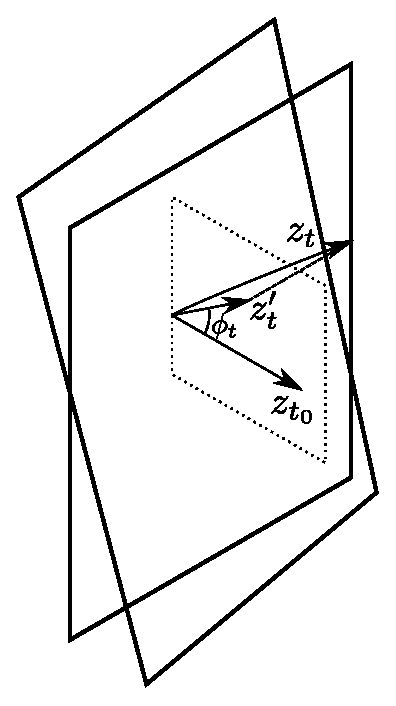
\includegraphics[width=0.3\linewidth]{./img/projection2.eps}
  \caption{Caso em que a rotação em torno de ${x}_c$ não representa a inclinação do plano do alvo.}
  \label{fig:projection}
\end{figure}%


Dada a matriz de rotação ${R}_{ct_0}$, do sistema de coordenadas da câmera ao sistema de coordenadas do alvo em sua posição inicial, mostrada na Figura \ref{fig:camera_ref}
\begin{equation}
{R}_{ct_0} = \m{ ({x}_{t_0})_c & ({y}_{t_0})_c  & ({z}_{t_0})_c} = 
\m{
	-1 & 0 & 0 \\
	0 & 1 & 0 \\
	0 & 0 & -1
}
%\m{
%  0 & 1 & 0 \\
%  1 & 0 & 0 \\
%  0 & 0 & -1
%}
\end{equation}
é conhecida a normal ao plano do alvo é ${n} = {x}_{t_0} \times {z}_{t_0} =  {y}_{t_0} $. A matriz de projeção linear \citep{strang} de um vetor em um plano é dada por
\begin{equation}
{P} = {I} - {n} {n}^T,
\end{equation}
logo para ${n} = {y}_{t_0}$ temos 
\begin{equation}
{P} =  \m{
	 0  &   0  &   0 \\
     0  &   1  &   0 \\
     0  &   0  &   1
}.
\end{equation}

O vetor projetado no plano é dado por
\begin{equation}
{z'}_{t} = {P} {z}_{t},
\end{equation}
assim basta apenas encontrar o ângulo entre os vetores ${z'}_{t}$ e ${z}_{t_0}$, que pode ser calculado pela fórmula do Cosseno \citep{strang} 
\begin{equation}
\phi_{et} = \cos^{-1} \left( \frac{{z'}^T_{t} {z}_{t_0} } {||{z'}_{t}|| \; ||{z}_{t_0}||} \right)
\end{equation}
%\begin{align}
%(\bm{p}_t)_e &= (\bm{p}_c)_e + (\bm{p}_t)_e \\
%(\bm{p}_t)_e &= (\bm{p}_c)_e + \bm{R}_{ec} (\bm{p}_t)_c 
%\end{align}
Após obter os valores de $(p_{et})_e$ e $\phi_{et}$, sabemos $(x_{et})_e$ e controle se resume a:
\begin{align}
x_\Delta &= ({x}_{et})_e - ({x}_{e^*t})_e\\
{\bar{u}} &= {K}_v {x_\Delta}  \\
{u} &= ({J}_{a})_e^{-1} {\bar{u}}
\end{align}

\section{Controle de Força} \label{sec:force}

Utilizando o sensor de força descrito em \ref{sec:optoforce}, montado no efetuador final do manipulador, deseja-se fazer o controle da força aplicada sobre uma superfície. 

A matriz de rotação do referencial do sensor para o referencial do efetuador, como definido em \ref{fig:modelo_tetis} é dada por

\begin{equation}
R_{es} = \m{
  0 & 0 & 1 \\
  0 & -1 & 0 \\
  1 & 0 & 0
}
\end{equation}

\subsection{Float}  \label{sec:forca_float}
Esse mode de controle de força consiste em configurar uma referência de controle de força ${f}_d = 0$, de modo que o efetuador do manipulador fique "flutuando", se movendo de forma sensível ao toque.

Primeiramente a força representada no referencial do sensor $({f})_s \in \mathbb{R}^3 $ é representada na base por $({f})_e = R_{es} ({f})_s$. Com ${f}_d = 0$, o erro fica
\begin{equation}
({e}_f)_e = - ({f})_e 
\end{equation}
Utilizando um controle proporcional:
\begin{align}
\bar{{u}}_f &= {K}_f ({e}_f)_e \\
\bar{{u}} &= \m{ \bar{{u}}_f & 0}^T\\
{u} &= ({J_a})_b^{-1} \bar{{u}}
\end{align}

\subsection{Approach} \label{sec:forca_approach}
Considera-se o problema de controle de força na direção de \textit{approach} para o manipulador robótico 4-DOF em questão. O objetivo de controle é resolver o problema de \textit{set-point}, ou seja, rastrear uma referência de força constante.

É possível modelar o ambiente (força de contato), ou seja, a placa de poliestireno, como uma mola linear, através da \textit{Lei de Hooke}: 
\begin{equation}
f = -k_s (x - x_s)
\end{equation}
onde $x$ é a posição do ponto de contato com a superfície e $x_s$ um ponto na superfície.

Considerando que o controle de força seja ativado somente após a etapa de contato com o ambiente onde será aplicada a força e que o controle de força é feito apenas na direção de approach (segundo o sistema de coordenadas $\bar{E}_e$, na direção $x$), pode-se utilizar a malha de controle mostrada na figura \ref{fig:controle_forca}. É utilizada uma lei de controle com ação proporcional e integral conforme a equação \eqref{eq:pi_force}.
%\begin{equation}
%\bar{u} = -K_s^{-1} (K_fe_f + K_i \int_0^t e_f(\tau)d\tau)
%\end{equation}


\begin{figure}[h!]
\centering
\begin{tikzpicture}[auto, node distance=2cm,>=latex']
    % We start by placing the blocks
    \node [input, name=input] {};
    \node [sum, right of=input] (sum) {};
    \node [block, right of=sum] (Ks1) {$k_s^{-1}$};
    \node [block, right of=Ks1] (C) {$C(s)$};
    \node [blockbig=right:C] (J) [right=1cm of C] {$(J_a)_e^{-1}$};
    \node [block=right:J] (Integral) [right=1cm of J] {$\int$};
    \node [blockbig, right of=Integral] (DirKine) {${k}(\cdot)$};

	\node [tmp=below:J] (tmp0) [below left=-1.25cm and .7cm of J] {};
	\node [tmp=below:J] (tmp00) [below left=-2cm and 0.7cm of J] {};
	\node [tmp=below:J] (tmp000) [below left=-2cm and 0cm of J] {};

    \node [tmp=below:J] (tmp1) [below left=-1.5cm and 0.5cm of J] {};
    \node [tmp=below:J] (tmp2) [below left=-1.5cm and 0cm of J] {};

    \node [tmp=below:J] (tmp3) [below left=-1cm and 0.5cm of J] {};
    \node [tmp=below:J] (tmp4) [below left=-1cm and 0cm of J] {};

    \node [tmp=below:J] (tmp5) [below left=-0.5cm and 0.5cm of J] {};
    \node [tmp=below:J] (tmp6) [below left=-0.5cm and 0cm of J] {};

    \node [tmp=below:J] (tmpk0) [below right=-2cm and 0cm of DirKine] {};
	\node [tmp=below:J] (tmpk00) [below right=-2cm and 0.7cm of DirKine] {};
	\node [tmp=below:J] (tmpk000) [below right=-1.25cm and 0.7cm of DirKine] {};

    \node [tmp=below:J] (tmpk1) [below right=-1.5cm and 0.5cm of DirKine] {};
    \node [tmp=below:J] (tmpk2) [below right=-1.5cm and 0cm of DirKine] {};

    \node [tmp=below:J] (tmpk3) [below right=-1cm and 0.5cm of DirKine] {};
    \node [tmp=below:J] (tmpk4) [below right=-1cm and 0cm of DirKine] {};

    \node [tmp=below:J] (tmpk5) [below right=-0.5cm and 0.5cm of DirKine] {};
    \node [tmp=below:J] (tmpk6) [below right=-0.5cm and 0cm of DirKine] {};


    \node [block=right:DirKine] (ks) [right=1cm of DirKine] {$k_s$};
    \node [output, right of=ks] (output) {};

    % Once the nodes are placed, connecting them is easy. 
    \draw [draw,->] (input) -- node {$f_d$} (sum);
    \draw [->] (sum) -- node {$e_f$} (Ks1);
    \draw [->] (Ks1) -- node {} (C);
    %\draw [->] (C) -- node[name=u] {$u$} (tmp0);
    \draw [->] (J) -- node {${\dot{q}}$} (Integral);
    \draw [->] (Integral) -- node {${q}$} (DirKine);
    \node [block, below of=J] (measurements) {$H(s)$};
    %draw [->] (DirKine) -- node {} (ks);
    \draw [->] (ks) -- node [name=x] {$f$}(output);
    \draw [->] (x) |- (measurements);
    \draw [->] (measurements) -| node[pos=0.99] {$-$} 
        node[near end] {$f_m$} (sum);

    \draw [->] (C) -- (tmp0) -|  (tmp00) |- node[pos=0.65] {$x$} (tmp000);

    \draw [->] (tmpk0) -- node[pos=0.2] {$x$} (tmpk00) -|  (tmpk000) |-  (ks);
    \draw [->] (tmp1) -- node[pos=0] {$y$} (tmp2);
    \draw [->] (tmp3) -- node[pos=0] {$z$} (tmp4);
    \draw [->] (tmp5) -- node[pos=0] {$\phi$} (tmp6);

    \draw [->] (tmpk2) -- node[pos=0.3] {$y$} (tmpk1);
    \draw [->] (tmpk4) -- node[pos=0.3] {$z$} (tmpk3);
    \draw [->] (tmpk6) -- node[pos=0.3] {$\phi$} (tmpk5);
    %\draw [->] (x) |- (tmp1) -| node[pos=0.9] {$-$} (sum);
\end{tikzpicture}
\caption{Diagrama de Blocos: Malha de Controle de Força.}
\label{fig:controle_forca}
\end{figure}

O diagrama da Figura \ref{fig:controle_forca} pode ser simplificado se abstrairmos as outras dimensões que não a de approach, resultando em \ref{fig:controle_forca_simples}.

\begin{figure}[h!]
\centering
\begin{tikzpicture}[auto, node distance=2cm,>=latex']
    % We start by placing the blocks
    \node [input, name=input] {};
    \node [sum, right of=input] (sum) {};
    \node [block, right of=sum] (Ks1) {$k_s^{-1}$};
    \node [block, right of=Ks1] (C) {$C(s)$};
    \node [block, right of=C] (PWM) {$k_s$};
    \node [block, right of=PWM] (Robo) {$\ddfrac{1}{s}$};
    \node [tmp, below of=K] (tmp1){};
    \node [output, right of=Robo] (output) {};

    % Once the nodes are placed, connecting them is easy. 
    \draw [draw,->] (input) -- node {$f_d$} (sum);
    \draw [->] (sum) -- node {$e_f$} (Ks1);
    \draw [->] (Ks1) -- node {} (C);
    \draw [->] (C) -- node[name=u] {$u$} (PWM);
    \node [block, below of=u] (measurements) {$H(s)$};
    \draw [->] (PWM) -- node [name=tau] {} (Robo);
    \draw [->] (Robo) -- node [name=x] {$f$}(output);
    \draw [->] (x) |- (measurements);
    \draw [->] (measurements) -| node[pos=0.99] {$-$} 
        node[near end] {$f_m$} (sum);
    %\draw [->] (x) |- (tmp1) -| node[pos=0.9] {$-$} (sum);
\end{tikzpicture}
\caption{Diagrama de Blocos: Malha de Controle de Força Simplificada.}
\label{fig:controle_forca_simples}
\end{figure}

Considerando $H(s) = 1$
\begin{equation}
G(s) = \frac{k_p s + k_i}{s^2 + k_p s + k_i}
\end{equation}

Como o sinal vindo do sensor é bastante ruidoso, utiliza-se um filtro de primeira ordem com $f_c = 1$.
\begin{equation}
H(s) = \frac{1}{\tau s + 1}
\end{equation}
onde $\tau = 1/(2 \pi f_c) \approx 0.16$.

Ficamos com a função de transferência a seguir a partir da qual é possível sintonizar os parâmetros do controlador.
\begin{equation}
G(s) = \frac{k_p \tau s^2 + (k_p + \tau k_i)s + k_i}{\tau s^3 + s^2 + k_p s + k_i}
\end{equation}

Considerando que obtemos do sensor de força um vetor $({f})_s \in \mathcal{R}^3$, representado no referencial do sensor. O controle de força pode ser implementado a partir das seguintes equações:
\begin{align}
({f})_e &= {R}_{es} ({f})_s \\
({e}_f)_e &= {f}_d - ({f})_e \\
\end{align}
A estratégia de controle PI é dada por
\begin{equation}
\bar{{u}}_f = -{K}_s^{-1} ({K}_f ({e}_f)_e + {K}_i \int_0^t ({e}_f)_e (\tau)d\tau)\\
\end{equation}
Como ${u} \in \mathcal{R}^4$  e desejamos controlar somente a direção de \textit{approach}:
\begin{equation}
\bar{{u}} = \m{ {S}_f \bar{{u}}_f \\ 0} 
\end{equation}
onde 
\begin{equation}
{S}_f = \m{
  1 & 0 & 0 \\
  0 & 0 & 0 \\
  0 & 0 & 0
},
\end{equation}
portanto:
\begin{equation}
{u} = ({J_a})_e^{-1} \bar{{u}}
\end{equation}

%Especificações:
%\section{Controle Híbrido}
%Considerando o diagrama \ref{fig:controle_forca}, é possível suprir os graus de liberdade não controlados $y$, $z$ e $\phi$ %com outra lei de controle, como por exemplo o um Proporcional com Feedforward de modo a aplicar uma força na direção de %approach e traçar uma trajetória de na superfície em que a força está sendo aplicada. 

%\section{Master-Slave (Omni)}
%TODO

% TODO: TABELA COM LEIS DE CONTROLE E FONTE DOS DADOS 
  \chapter{Descrição do Hardware}

Nesse capítulo serão descritos elementos do hardware associados ao funcionamento do manipulador TETIS. A descrição completa dos dispositivos do robô DORIS, pode ser obtida em \cite{xaud2016doris}.

\section{Sistema Elétrico}

Rede Local \textit{Gigabit Ethernet}. È responsável pela comunicação de alta largura de banda entre o DORIS e seus diversos periféricos. A essa rede estão conectados o computador embarcado, cameras \textit{Ethernet}, access points Wi-Fi, roteadores, o \textit{Vehicle Support System} (VSS).

Sistema de atuação. É responsável pela atuação dos motores do DORIS. É composto pelo subsistema de tração e pelo subsistema do manipulador. 

\textit{Controller Area Network (CAN)} É responsável pelo controle em tempo real do sistema de atuação através de uma rede robusta. A rede CAN integra os drivers do sistema de atuação e os computadores embarcados em uma topologia de rede em barramento. 

Rede de computadores: O projeto inicial do DORIS incluia dois módulos PCIe/104 com Intel \texttrademark Core i7 e discos de estado sólido (SSD). Atualmente ele está operando com um módulo PCIe/104 Intel Atom D525. 


\section{Atuadores e Drivers}

As juntas de revolução do TETIS necessitam de atuadores com as seguintes características:

\begin{itemize}
\item Alto taxa de redução, para permitir controle a nível de velocidade nas juntas.
\item Folga desprezível, para evitar a adição de não linearidades ao sistema. 
\item Eixo oco para permitir o roteamento de cabos através dele.
\item Alta acurácia e repetibilidade
\end{itemize}

A tecnologia \textit{Harmonic gear}, registrada pela \textit{Harmonic Drive}, consiste em engrenagens do tipo \textit{strain wave}. Esse mecanismo melhora certas características em comparação com sistemas de transmissão tradicionais como engrenagens helicoidais, ou planetárias. As vantagens incluem a inexistência de folgas, mais compacto, leve, altas taxas de redução, excelente resolução e repetibilidade, alto torque.

O manipulador TETIS se baseia nos atuadores \textit{FHA Mini Servo} da \textit{Harmonic Drive AG}, mostrados na figura \ref{fig:harmonic_drive}. Esse atuador cumpre os requisitos acima. Ele conta também com \textit{encoder}, montado no eixo do motor antes da redução, e sensores \textit{hall} para os três enrolamentos. Com base nos requisitos de torque, para as duas primeiras juntas é utilizado o modelo FHA-11C-100-D200-EKMI, enquanto que para as duas úlimas o modelo FHA-8C-100-D200-EKMI.

Para atinjir um controle satisfatório a nível de junta, são utilizados drivers da Maxon Motor, compatíveis com o barramento CAN. Cada junta é controlada por um driver modelo Maxon Motor EPOS2 70/10 P/N 375711, mostrado na figura \ref{fig:harmonic_drive}.

\section{Câmera Minoru} \label{sec:minoru}

O robô DORIS conta com diversos tipos de câmeras, como camera de alta definição, térmica, \textit{fisheye} e estereoscópica. 

A figura \ref{fig:efet_minoru} mostra a câmera utilizada para o controle por servovisão e o efetuador com a câmera montada.
A câmera em questão é a \textit{Minoru 3D Webcam}, uma câmera esterescópica que possui dois sensores VGA CMOS. É um dispositivo leve que pode ser acoplado ao efetuador final.

\begin{figure}[H]
\centering
\begin{subfigure}{.5\textwidth}
  \centering
  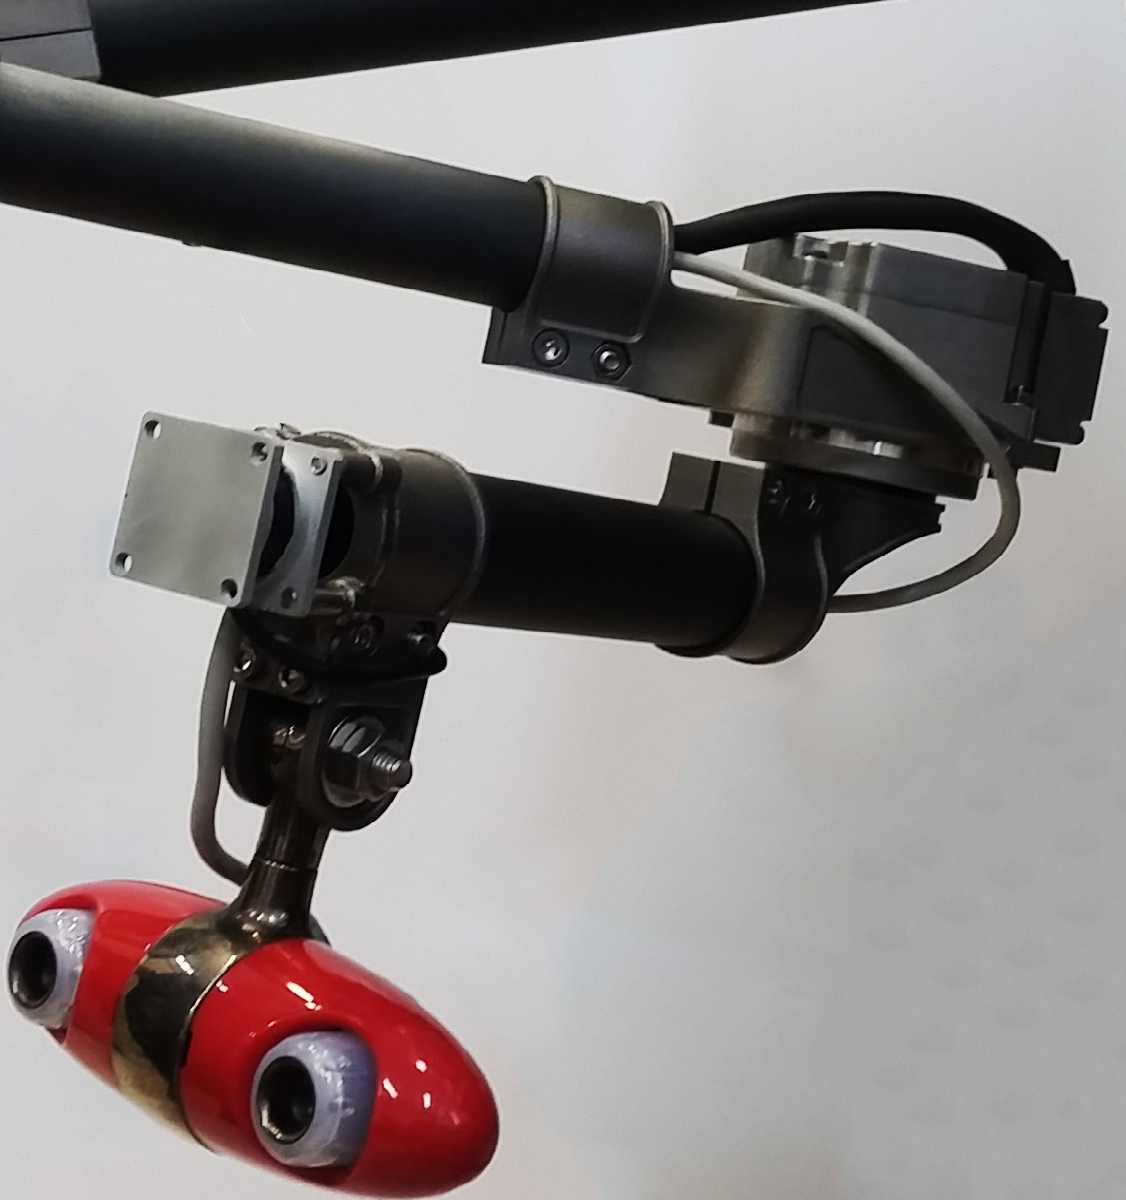
\includegraphics[width=0.75\linewidth]{./img/manip_zoom.png}
  \caption{Efetuador com câmera}
  \label{fig:efetuador}
\end{subfigure}%
\begin{subfigure}{.5\textwidth}
  \centering
  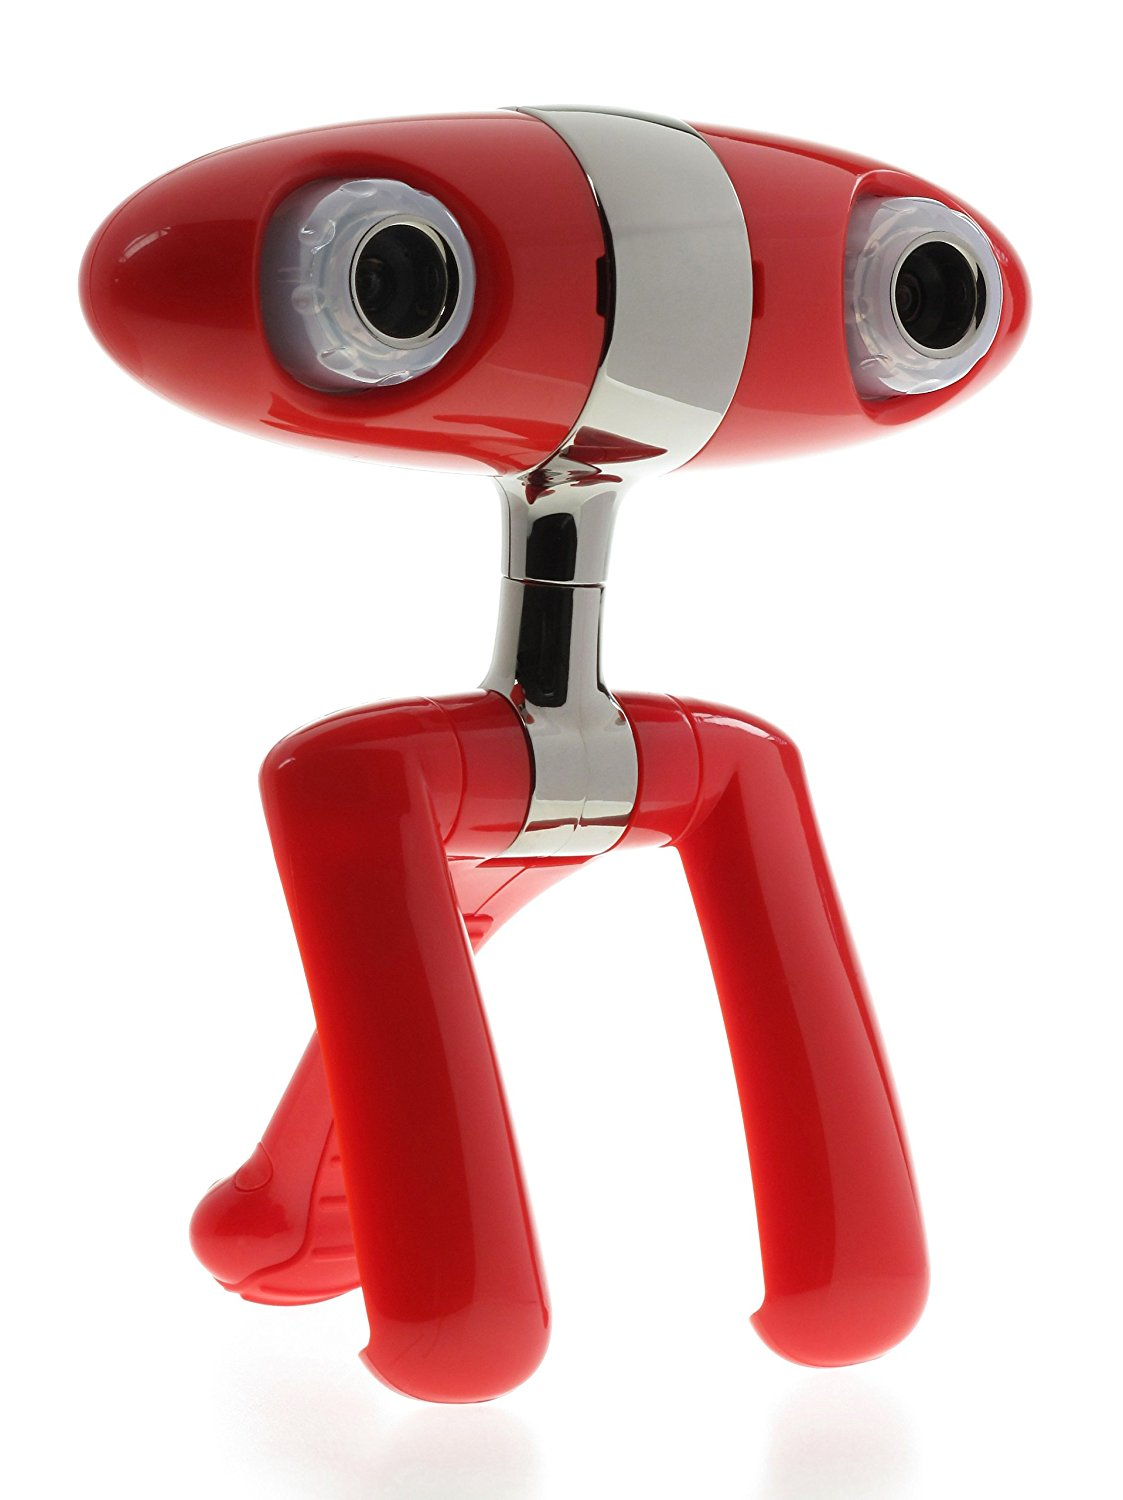
\includegraphics[width=0.6\linewidth]{./img/minoru.jpg}
  \caption{Minoru Camera}
  \label{fig:minoru}
\end{subfigure}
\label{fig:efet_minoru}
\caption{Efetuador e câmera Minoru}
\end{figure}

\section{Sensor de Força}

No efetuador do manipulador TETIS há um sensor de força da \textit{OptoForce Kft.}, modelo OMD-20-FE-200N. Os sensores Optoforce 3D medem a magnitude e direção de forças $F_x$, $F_y$ e $F_z$ utilizando princípios ópticos \cite{optoforce}. O sensor utiliza uma interface USB. 

\begin{figure}[!ht]
\centering
  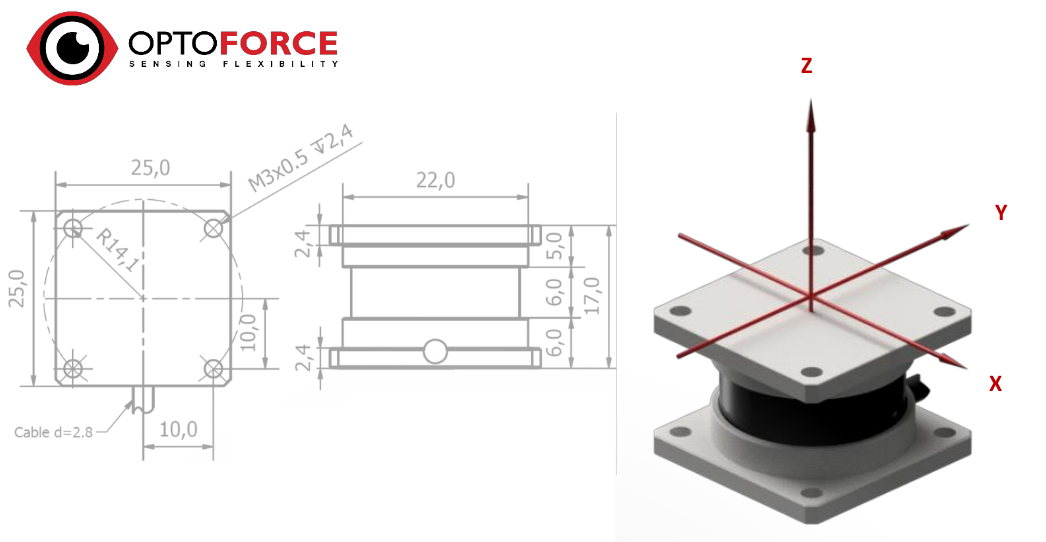
\includegraphics[width=\linewidth]{./img/optoforce.png}
  \caption{Optoforce OMD-20-FE-200N \cite{optoforce}}
  \label{fig:optoforce}
\end{figure}%

\begin{table}[h!]
\centering
\caption{Capacidade do sensor Optoforce OMD-20-FE-200N}
\label{tab:dh_tetis}
\begin{tabular}{rrrrr} \hline
 &  Capacidade Nominal & Deformação Típica \\ \hline
 $F_{xy}$ & $\pm 20N$ & $\pm 1.5 mm$ \\
 $F_z $ - Compressão & $200N$ & $1.2 mm$ \\
 $F_z $ - Tensão & $100N$ & $1 mm$ \\
\hline
\end{tabular}
\end{table}


\section{Integração dos dispositivos}

A malha de controle do manipulador TETIS é integrada através da \textit{Controller Area Network} (CAN) e da interface USB do computador embarcado PCIe/104. O computador é o nó principal, recebendo dados de sensores e enviando comandos de controle para os drivers.

Através da interface USB, o computador recebe realimentação do sensor de força e vídeo da câmera. A realimentação dos encoders é feita através do barramento CAN, passando pelos drivers EPOS2. A figura \ref{fig:integration} ilustra a integração do manipulador ao sistema do robô.

\begin{figure}[!ht]
\centering
  \includegraphics[width=\linewidth]{./img/integration_diagram}
  \caption{Esquema de integração dos dispositivos.}
  \label{fig:optoforce}
\end{figure}%
  \chapter{Implementação}
A implementação dos algoritmos de controle detalhados nos capítulos anteriores for feita como extensão ao software RobotGUI desenvolvido pela equipe do LEAD-GSCAR, idealizado por Alex F. Neves Msc. 

%\section{Motivação} 
%Modular, genérico, ...

\section{Ferramentas}
Os seguintes softwares e \textit{frameworks} foram utilizados:

\begin{itemize}
\item Linux (Ubuntu) como Sistema Operacional
\item C++ como linguagem de programação
\item ROS como \textit{framework} principal utilizado o RobotGUI, fornecendo comunicação entre nós através de mensagens e serviços. Será descrito mais detalhadamente na próxima seção.
\item Qt como \textit{framework} para elaboração da interface gráfica. 
\end{itemize}

\section{ROS}

\section{Conceitos}

Primeiramente define-se como Computador Base aquele que será utilizado pelo operador para controlar e visualizar dados do robô. Define-se Computador Embarcado, ou do Robô aquele que está no robô conectado a todos os equipamentos, sensores e atuadores. O software executa módulos diferentes no robô e na base.

A arquitetura do RobotGUI baseia-se nos seguintes conceitos principais:

\begin{itemize}
\item \textbf{Components}: Lidam com a comunicação e processam dados no Computador Base. São essencialmente \textit{Nodelets} de ROS, podendo utilizar funcionalidades como comunicação através de mensagens e serviços, utilizar parametros e bibliotecas de ROS. Permitem maior modularidade pois comonentes podem ser inicializados independentemente do \textit{RobotGUI}.

\item \textbf{Tools:} São elementos gráficos da interface para o usuário. São utilizadas para interagir com o robô e visualizar informação. São criadas como \textit{plugins} para o ROS \textit{pluginlib} e independetes de qualquer biblioteca do ROS.

\item \textbf{Interação entre Compontents e Tools:} Tools e Components podem se conectar, quando isso ocorre eles interagem entre si a nível de "ponteiro para objeto". Essa conecção permite que o desenvolvimento da interface através do \textit{Qt} seja quase que independente do desenvolvimento do código que lida com hardware, lógica e comunicação.

\item \textbf{RobotGUI}
\end{itemize}


\section{Modos de Controle}

\subsection{Velocidade no Espaço Operacional}
\subsubsection{Base}
\subsubsection{Efetuador}
\subsection{Posição no Espaço das Juntas}
\subsection{Posição no Espaço Operacional}
\subsection{Rastreamento de Trajetória}
\subsection{Servo Visão}
\subsection{Força}
\subsubsection{Float}
\subsubsection{Approach}
\subsubsection{Híbrido}
\subsection{Master-Slave (Omni)}
  \chapter{Resultados e Discussões}

\section{Respostas das Juntas}
Para verificar se de fato são válidas as premissas assumidas na seção \ref{sec:controle_cinematico} para aplicação de uma estratégia de controle cinemático foi levantada para cada uma das juntas a resposta a uma onda quadrada tal que:
\[ u = A \sgn(\sin( 2\pi t/f)) \]
onde o período $T = 1/f = 1s$ e a amplitude $A = 0.5 rad/s$

\newlength{\imageheight}
\begin{figure}[!ht]
  \centering
  	\settoheight{\imageheight}{\includegraphics{./img/joints}}
    \includegraphics[width=\textwidth, clip=true, trim = 0 0.5\imageheight 0 0 0 mm]{./img/joints}
  \caption{Resposta das juntas}
\end{figure}


  \chapter{Conclusões e Trabalhos Futuros}

\section{Conclusões}

Neste projeto de graduação foi apresentada a modelagem cinemática, estratégias de controle baseadas na abordagem de controle cinemático, assim como a implementação de um software para controle de sistemas robóticos, utilizando como estudo de caso o manipulador TETIS, do sistema DORIS. 

A modelagem cinemática consiste em representar o manipulador como uma cadeia cinemática de corpos rígidos, de modo a obter relações geométricas que governam o sistema. A cinemática direta do manipulador TETIS foi obtida através da convenção Denavit–Hartenberg. Diferenciando as equações resultantes com respeito as variáveis das juntas foi possível obter a cinemática diferencial, relacionando a velocidade no espaço operacional com as variáveis de juntas, na forma do Jacobiano analítico. Em simulação os resultados se mostraram compatíveis com o esperado. 

A abordagem de controle cinemático assume que é possível considerar um sistema cinemático como entrada do sistema, tipicamente um valor de velocidade. Isso é possível quando existe uma malha de controle de baixo nível, que idealmente é capaz de impor uma velocidade especificada de referência. Esse é o caso do TETIS, que utiliza atuadores \textit{FHA Mini Servo} com drivers EPOS2 70/10, com uma malha de baixo nível de velocidade. Assim, utilizou-se como modelo simplificado do robô um integrador, supondo que os servos são capazes de reproduzir comandos de velocidade de forma razoavelmente precisa. No caso da junta 2, essa reprodução não é tão precisa devido necessidade de maior torque, por estar no início da cadeia.

O rastreamento de trajetória com controle proporcional com \textit{feedforward} apresentou erro em regime permanente pelos seguintes fatores: (i) ciclo de controle máximo que o computador embarcado suporta é de $10ms$; (ii) Junta 2 não é capaz de reproduzir com tanta precisão comandos de velocidade, por estar mais sujeita à força gravitacional; (iii) Ciclo de controle está sujeito a atrasos devido a interrupções do sistema operacional. 

Os componentes de software para controle, interação e configuração de parâmetros foram desenvolvidos e integrados ao RobotGUI, que já era utilizado para controle dos demais sistemas do robô. A interface gráfica permite a visualização de dados de forma gráfica \textit{online} dos sinais, assim como a reconfiguração de parâmetros no computador embarcado com aquelas desejadas. A adição de novas funcionalidades e modos de controle é imediata, devido a arquitetura modular e ao paradigma orientado a objetos. O ROS segue os princípios de um microkernel, onde as funcionalidades são implementadas separadamente em módulos bem definidos que se comunicam, em contraste com um "monolito" que realiza todas as funções. Isso permite que nós possam ser substituidos ou modificados sem influenciar outros, desde que sigam o mesmo protocolo (tópicos/serviços). Por exemplo, caso seja de interesse substituir o módulo de visão computacional basta publicar/subscrever aos mesmos tópicos.

A implementação de software para controle com computação em tempo real é custosa em tempo de implementação e pouco expansível, necessitando tratar de algoritmos de \textit{scheduling} e latência de entrada/saída \citep{nilsson1998real}. A abordagem utilizada neste trabalho permite uma implementação mais desacoplada e menos interdependente. No entanto, existem algumas desvantagens do uso do ROS para um software completamente desacoplado. Existem \textit{overheads} de comunicação entre \textit{ROS Nodes}, que pode se tornar crítico no caso de separar o nó de controle do nó de atuação, conforme mostrado no apêndice \ref{chap:delay}. Essa separação introduziria atrasos significativos, tornando-se evidente para o caso em que o objetivo de controle é rastrear uma trajetória que é função do tempo. Em casos como nó de visão computacional que realiza o processamento de imagem a separação é inevitável e não representa um problema. Conclui-se ser mais apropriado juntar os nós de atuação e controle, o que melhorou significativamente o erro de rastreamento. %, já que o tempo de processamento já é 

Com o uso do Julia Language foi possível alterar em tempo de execução a trajetória a ser rastreada escrevendo as equações em uma janela na interface, com uma sintaxe simples. O \textit{script} é compilado \textit{just-in-time} e pode ser executado sem perda de performance.
%Com base nos resultados obtidos:
%Quando se necessita de ROS nem sempre é uma solução adequada,

\section{Trabalhos futuros}
\begin{itemize}
\item Modelo dinâmico do manipulador TETIS.

\item Utilizar ambos os sensores da cãmera estereoscópica Minoru de modo a melhorar a estimação da posição e orientação de um alvo, assim como ampliar o campo de visão.

\item Extender o uso do Julia Language, de modo a tornar o controle ainda mais dinâmico. Atualmente é utilizado somente na definição de uma trajetória a ser rastreada, no entanto é possível implementar algoritmos de controle inteiramente no Julia, o que permitiria ajustes e experimentos em tempo de execução.

\item Estudar implementações para sistemas de controle em tempo real e como tratar atrasos de entrada/saída.
\item Integrar o \textit{Sensable Phantom Omni}, um dispositivo háptico, em modo Master/Slave.
\end{itemize}

%A cinemática direta expressa a posição e orientação do efetuador final em função das variáveis de junta, enquanto que a cinemática diferencial fornece a relação entre a velocidade das juntas e a velocidade do efetuador final.

  
  \backmatter
  \bibliographystyle{agsm}
  \bibliography{thesis}

  \appendix
  %\chapter{Algumas Demonstra{\c c}\~oes}
%\chapter{Estimação da posição e orientação}
\chapter{Estimação da \textit{pose} em tempo real}  \label{chap:pose_est}
\section{ViSP - Visual Servoing Platform}

Para a implementação do modo de controle por Servo Visão, foi utilizada a biblioteca ViSP. A ViSP contém um módulo de visão computacional que permite computar a \textit{pose} de um objeto a ser reconhecido por meio de um padrão pre-determindado. São utilizados algoritmos robustos e fornecidos mecanismos para calibração da câmera. Esse módulo em alguns casos funciona como um envoltório para a biblioteca OpenCV, de modo a facilitar sua aplicação em problemas de robótica. 

As seguintes abordagens ao problema PnP estão disponíveis
\begin{itemize}
\item Abordagem Linear Lagrange. É realizado um teste para verificar aplicação da versão planar ou não-planar do algoritmo. 
\item Abordagem Linear Dementhon \cite{dementhon1995model} \cite{oberkampf1996iterative}  É realizado um teste para verificar aplicação da versão planar ou não-planar do algoritmo. 
\item Abordagem Lowe baseada em um esquema de minimização não linear de Levenberg Marquartd. Precisa de inicialização por meio de Lagrange ou Dementhon.
\item  Abordagem de Lowe Não Linear inicializada pela aboradagem de Lagrange.
\end{itemize}

\section{OpenCV}
TODO


\section{visp\_auto\_tracker}
\end{document}